\documentclass{article}

% if you need to pass options to natbib, use, e.g.:
%     \PassOptionsToPackage{numbers, compress}{natbib}
% before loading neurips_2026

% arXiv preprint version (page numbers shown, no anonymous watermark)
\usepackage[preprint]{neurips_2026}

% to compile a preprint version, e.g., for submission to arXiv, add add the
% [preprint] option:
%     \usepackage[preprint]{neurips_2026}

% to compile a camera-ready version, add the [final] option, e.g.:
%     \usepackage[final]{neurips_2026}

% to avoid loading the natbib package, add option nonatbib:
%    \usepackage[nonatbib]{neurips_2026}

\usepackage[utf8]{inputenc} % allow utf-8 input
\usepackage[T1]{fontenc}    % use 8-bit T1 fonts
\usepackage{hyperref}       % hyperlinks
\usepackage{url}            % simple URL typesetting
\usepackage{booktabs}       % professional-quality tables
\usepackage{amsmath}        % advanced math typesetting
\usepackage{amssymb}        % math symbols
\usepackage{amsthm}         % theorem environments
\theoremstyle{plain}
\newtheorem{proposition}{Proposition}
\theoremstyle{definition}
\newtheorem{assumption}{Assumption}
\usepackage{amsfonts}       % blackboard math symbols
\usepackage{nicefrac}       % compact symbols for 1/2, etc.
\usepackage{microtype}      % microtypography
\usepackage{xcolor}         % colors
\usepackage{graphicx}       % include graphics
\usepackage{multirow}       % multirow tables
\usepackage{subcaption}     % subfigures
\usepackage{float}          % float placement
\usepackage{placeins}       % float barriers
\usepackage{dblfloatfix}    % improved placement for figure*

\newcommand{\melon}{MELON}

\hbadness=10000

\title{MELON: Multimodal Learning Framework for Spatial Multimodal Omics Data Integration}

% The \author macro works with any number of authors. There are two commands
% used to separate the names and addresses of multiple authors: \And and \AND.
%
% Using \And between authors leaves it to LaTeX to determine where to break the
% lines. Using \AND forces a line break at that point. So, if LaTeX puts 3 of 4
% authors names on the first line, and the last on the second line, try using
% \AND instead of \And before the third author name.

\author{%
  Yuchen~Zhang \\
  UTHealth Houston \\
  \texttt{yuchen.zhang@uth.tmc.edu} \\
  \And
  Chunru~Lin \\
  MD Anderson Cancer Center \\
  \texttt{clin2@mdanderson.org} \\
  \And
  Liuqing~Yang \\
  MD Anderson Cancer Center \\
  \texttt{lyang7@mdanderson.org} \\
  \AND
  Manu~Sebastian \\
  MD Anderson Cancer Center \\
  \texttt{mmsebastian@mdanderson.org} \\
  \And
  Yuying~Xie \\
  Michigan State University \\
  \texttt{xyy@msu.edu} \\
  \And
  Yu~Shen \\
  MD Anderson Cancer Center \\
  \texttt{yshen@mdanderson.org} \\
  \And
  Lulu~Shang \\
  MD Anderson Cancer Center \\
  \texttt{LShang@mdanderson.org} \\
}

\begin{document}

\maketitle

\begin{abstract}
  Recent advances in spatial omics technologies enable multiple molecular modalities to be measured on the same tissue section, providing
  complementary measurements of tissue organization. A central challenge is to integrate heterogeneous modalities, such as gene expression and chromatin accessibility, while preserving spatial structure and biological coherence. Here, we propose MELON, a representation-learning framework for spatial multi-omics integration that combines spatially aware graph attention with contrastive learning to learn shared spot-level embeddings for spatial domain detection. MELON uses modality-specific encoders together with a $k$-nearest-neighbor spatial graph, where learned edge gating and multi-head attention selectively aggregate information from informative spatial neighbors. Stochastic
  augmentations and a contrastive objective are then used to align modality-specific embeddings into a common latent space, which is subsequently clustered and compared against anatomical reference annotations. We evaluate MELON on three spatial multi-omics datasets using metrics including adjusted Rand index (ARI), spatial ARI, normalized mutual
  information (NMI), adjusted mutual information (AMI), V-measure, and homogeneity, and benchmark against established integration methods. Across datasets, MELON achieves consistently higher agreement with reference labels, yielding relative ARI gains over the best competing baseline of roughly 32\% on an E15 mouse brain dataset, 19\% on a human lymph node dataset, and 11\% on an E13 mouse embryo dataset. On the MISAR-seq E15 mouse brain dataset, MELON produces more spatially contiguous domains with sharper boundaries that better align with anatomical structures than competing baselines. These results demonstrate that MELON effectively leverages spatial multi-omic signals to enable accurate and interpretable tissue domain characterization.
\end{abstract}

\section{Introduction}

Multimodal spatial omics technologies represent a paradigm shift in understanding complex biological systems. They integrate diverse molecular and morphological modalities from the same tissue section while preserving the spatial layout of the tissue, enabling the study of cellular identity, regulatory state, and microenvironmental organization in situ. Representative spatial multi-omics settings now include transcriptome--proteome measurements in lymphoid tissue, transcriptome--epigenome assays such as spatial ATAC--RNA-seq, and transcriptome--histology integration settings that combine molecular profiles with tissue morphology \cite{long2024spatialglue,zhang2023spatial,zuo2023misar,coleman2025miso}. A key analysis task is spatial clustering or spatial domain identification, which aims to group spatial locations into biologically meaningful regions or cell-state neighborhoods. This task can be naturally framed as a multi-modality representation learning problem. Each modality provides a distinct layer of biological insight, for example, gene expression captures transcriptional output, while a paired modality such as chromatin accessibility, protein abundance, or hematoxylin and eosin (H$\&$E)-stained histology image captures complementary regulatory, phenotypic, or structural information. Effectively integrating these heterogeneous modalities is therefore central to producing biologically meaningful clusters.

Early attempts at multimodal clustering primarily relied on unsupervised methods developed for non-spatial multimodal data, such as Seurat WNN, MOFA+, and TotalVI \cite{hao2021seurat,argelaguet2020mofa,gayoso2021totalvi}, and then applied them to paired profiles while ignoring spatial dependencies between locations. Seurat WNN learns cell-specific modality weights and multimodal neighbor graphs for integrative analysis, MOFA+ uses a latent factor model to reconstruct a shared low-dimensional representation across multiple modalities, and TotalVI uses a variational probabilistic model to jointly analyze paired RNA and protein measurements. These methods are effective for multimodal integration in single-cell settings, but they do not explicitly model the spatial organization that is intrinsic to tissue slices. MEFISTO extends factor analysis to incorporate known spatial or temporal covariates and separate smooth from non-smooth variation \cite{velten2022mefisto}, partially addressing this limitation, but it remains fundamentally a low-rank factor model rather than a dedicated spatial multimodal clustering framework.

More recently, graph-based and deep multimodal models have become the dominant paradigm for spatial multiomics analysis because they can jointly encode neighborhood structure and heterogeneous molecular modalities in a learned latent space. For example, SpatialGlue constructs spatial neighbor graphs and uses attention-based fusion to integrate modality-specific embeddings for spatial domain identification \cite{long2024spatialglue}. Building on this direction, MultiGATE uses a two-level graph attention autoencoder that combines cross-modality feature relationships with spatial context, enabling both spatial embedding and cross-modality regulatory inference \cite{miao2025multigate}. In a related but broader multimodal integration setting, MISO proposes a deep framework for combining spatial molecular measurements with H\&E-derived morphological information \cite{coleman2025miso}. Across diverse datasets and platforms, these deep integration models have consistently achieved strong clustering or spatial reconstruction performance, highlighting the effectiveness of learning multimodal embeddings over spatial graphs or spatially informed architectures.

However, existing spatial multimodal clustering methods mainly optimize for a shared latent representation under spatial smoothness priors, but often fail to preserve modality-specific and cross-modal synergistic signals. In spatial multi-omics, this is a substantial limitation: spots with similar transcriptomes can differ in chromatin accessibility, protein abundance, or tissue morphology, reflecting distinct regulatory programs, signaling states, or microenvironmental contexts. For example, accessible enhancers may indicate lineage priming before RNA changes are detectable, protein levels may reflect post-transcriptional regulation not captured by gene expression, and histology may reveal stromal or immune tissue structure only weakly correlated with molecular profiles. As a result, methods that prioritize consensus structure can collapse biologically distinct spots into the same cluster. In previous methods, most existing objectives are based on alignment, reconstruction, or shared embedding and therefore emphasize redundant information, and modality interactions in tissue are often spatially dependent, becoming informative only in the context of local cellular neighborhoods.

To address this problem, we propose MELON (Multi-modal lEarning framework for spatial muLti-Omics integratioN), a spatially aware framework for clustering paired multimodal spatial data while preserving shared, modality-specific, and importantly, synergistic information. MELON first applies modality-specific encoders to each molecular or imaging modality, allowing each modality to retain its own structure and noise characteristics. It then uses a neighborhood-aware graph attention module to encode local tissue organization and learn which neighboring spots are most informative for each location. These embeddings are projected into a common latent space and fused with a transformer that models higher-order nonlinear dependencies across modalities. To reduce spurious neighborhood effects, MELON injects learned spatial attention weights as an adaptive bias into the fusion process. Finally, it uses a partial information decomposition (PID)-guided~\cite{williams2010nonnegative,bertschinger2014quantifying} multi-modality contrastive objective (built on multi-modality contrastive learning~\cite{tian2020contrastive} and the modality-masked PID-aware loss of~\cite{dufumier2024align}) over unimodal and multimodal masked inputs to encourage the learned representation to retain redundant, unique, and synergistic signal rather than collapsing to what the modalities share. This provides embeddings that preserve shared, modality-specific, and synergistic information, better resolve spatial regions supported by complementary signals across modalities. Figure~\ref{fig:overview} summarizes the spatial multi-omics task, MELON's spatial interaction and PID-guided fusion modules, and example downstream applications.

\begin{figure}[h!]
\centering
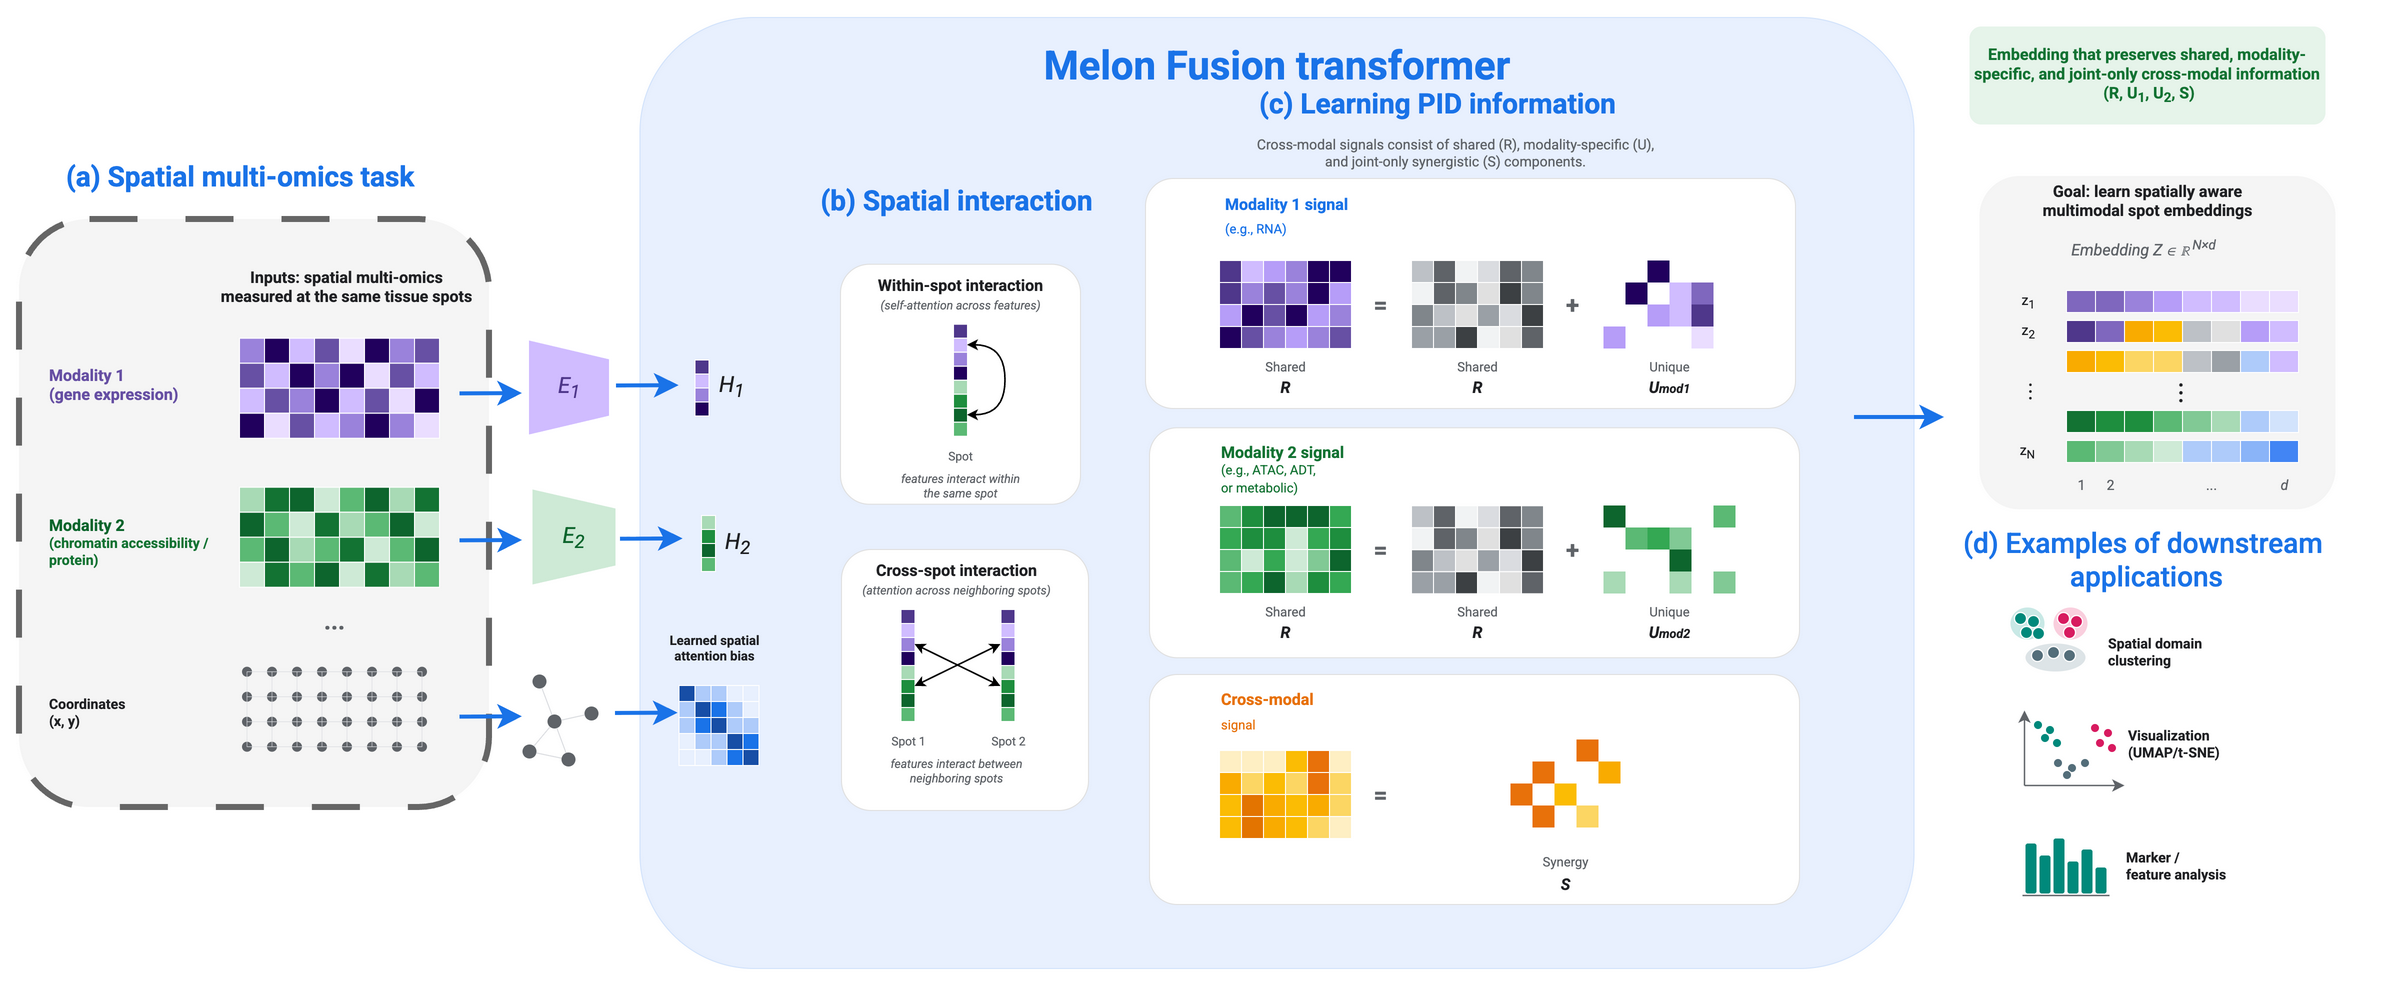
\includegraphics[width=\linewidth]{figures/figure_1_preview.png}
\caption{Overview of MELON. (a) Spatial multi-omics task: paired modality measurements (e.g., gene expression with chromatin accessibility or protein) on a tissue section, together with 2D spatial coordinates. (b) Spatial interaction: NeighborhoodGAT learns within-spot and cross-spot attention to encode local tissue organization and produce a learned spatial attention bias. (c) Learning PID information: a fusion transformer combined with a PID-guided multi-modality contrastive objective preserves shared, modality-specific, and synergistic signals across modalities. (d) Examples of downstream applications, including spatial domain clustering, visualization, and marker/feature analysis.}
\label{fig:overview}
\end{figure}

We evaluate MELON on paired spatial multimodal datasets spanning molecular--molecular and molecular--image settings, measuring clustering accuracy, spatial coherence, robustness across modality combinations, and biological interpretability. Our contributions are:
\begin{itemize}
  \item We formulate spatial multi-omics integration as a spatially aware multimodal representation learning problem that requires preserving shared, modality-specific, and synergistic cross-modal information.
  \item We propose MELON, which injects a learned neighborhood-aware spatial bias directly into multimodal fusion-transformer attention, and prove that this spatially biased variant inherits the PID recovery guarantee of prior PID-aware contrastive objectives.
  \item On controlled simulations isolating cross-modal synergy, MELON recovers a synergy-only label where all multimodal baselines operate at chance level, empirically confirming the preservation of synergistic information.
  \item On real spatial multi-omics data, MELON produces more accurate, spatially coherent, and biologically interpretable spot embeddings than strong multimodal baselines across molecular--molecular and molecular--protein settings.
\end{itemize}

\section{Related Work}

This section summarizes recent related works from three aspects: (1) spatial multi-omics integration, (2) contrastive representation learning (InfoNCE, SimCLR, CLIP, and PID-guided variants), and (3) spatial inductive biases for spatially resolved transcriptomics. Please refer to Appendix~\ref{app:related_work} for a more detailed discussion.

\section{Methods}
We present MELON, a spatial multimodal framework for learning spot embeddings from paired molecular profiles and spatial coordinates. MELON encodes each modality with a separate encoder, computes a learned spatial bias with NeighborhoodGAT, fuses the resulting tokens with a transformer that takes the spatial bias as an additive attention term, and trains the resulting embeddings with a multi-modality contrastive objective adapted from~\cite{dufumier2024align}. Our methodological contribution over standard multi-modality contrastive learning is a learned NeighborhoodGAT spatial bias that is injected directly into the fusion-transformer attention, making the spot embedding spatially aware rather than spatially blind. Figure~\ref{fig:melon-framework} shows the framework overview; preprocessing, augmentation formulas, token layouts, and architectural details are deferred to Appendix~\ref{app:impl}.

\begin{figure}[h!]
\centering
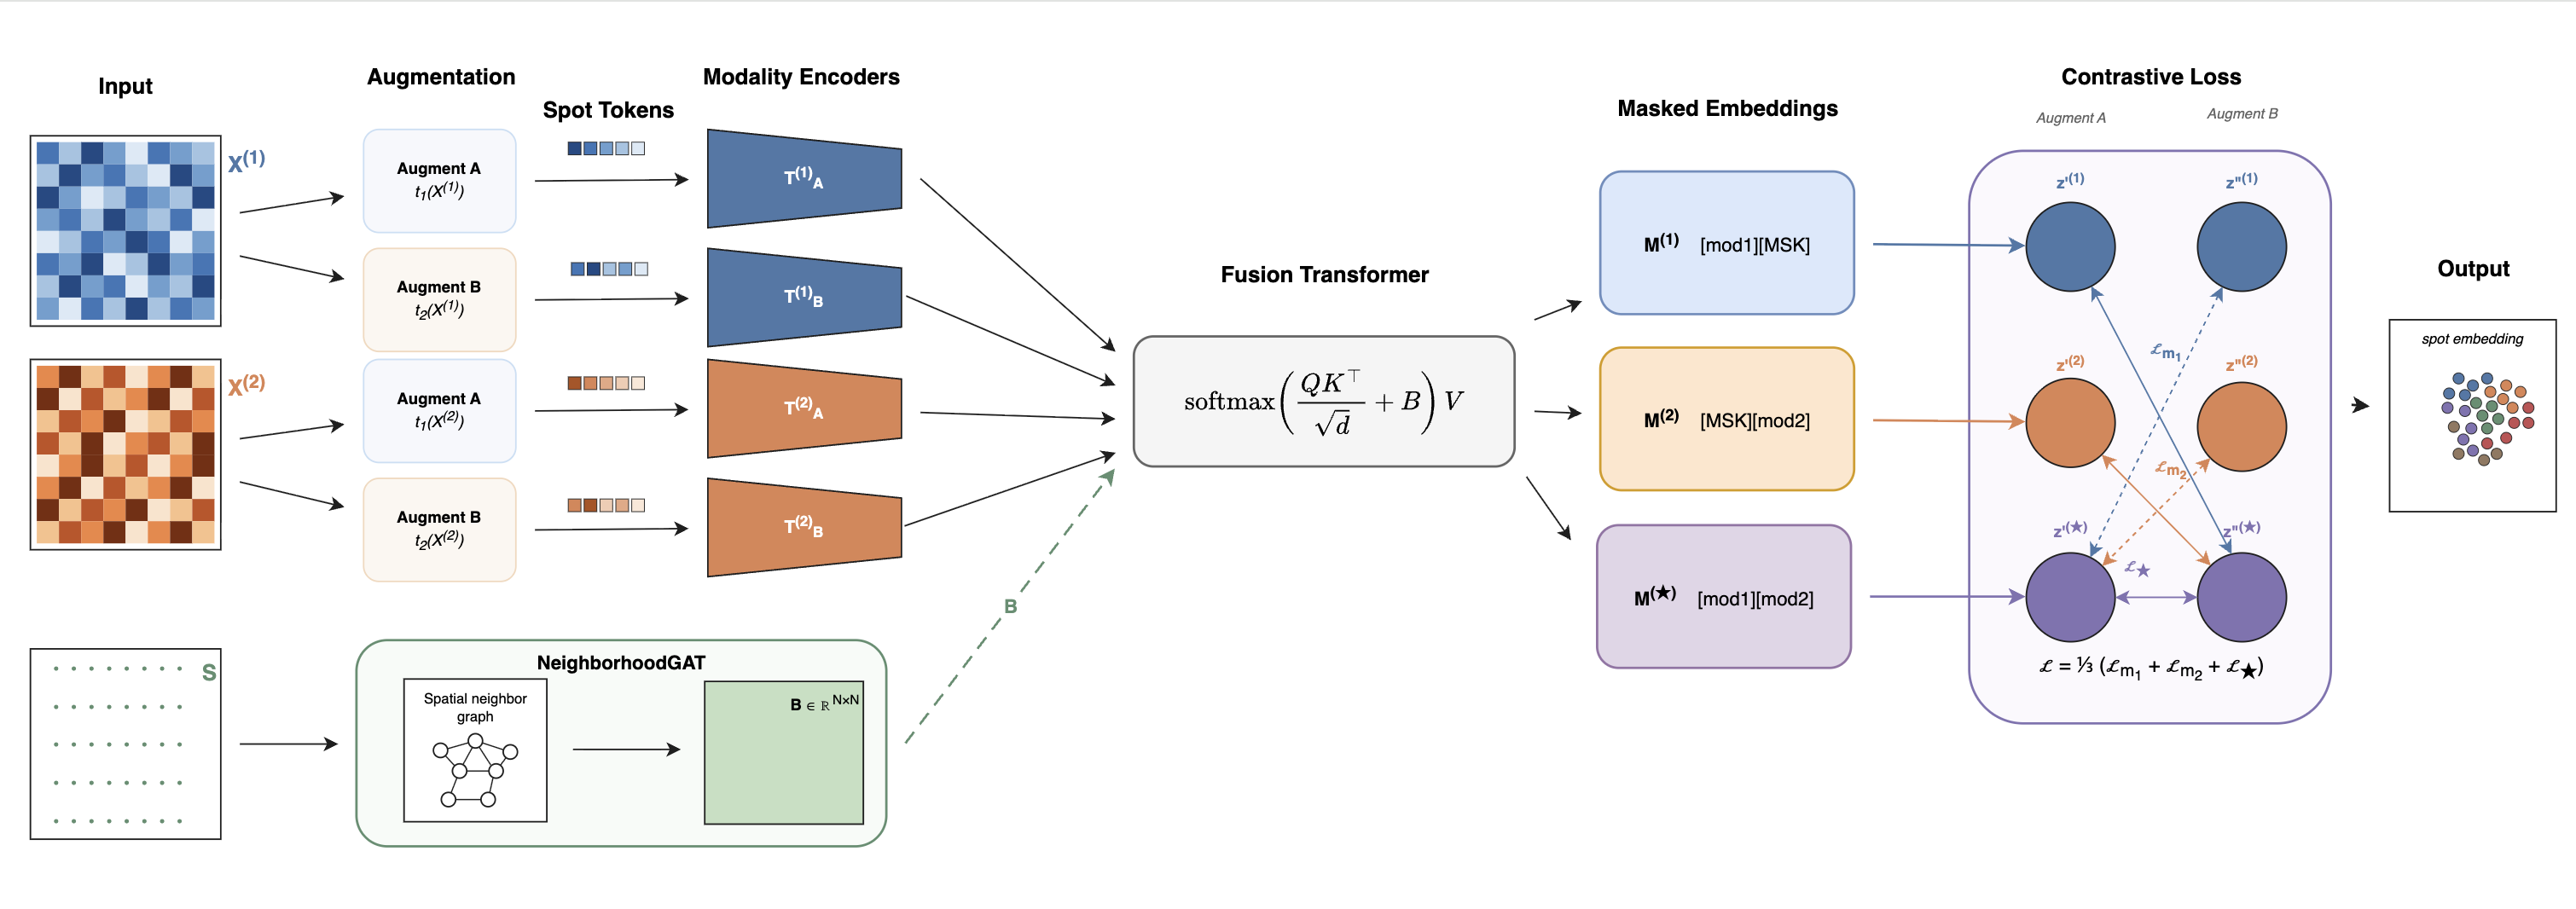
\includegraphics[width=0.96\columnwidth]{figures/framwork.png}
\caption{Overview of the MELON framework. The end-to-end pipeline takes paired spatial multimodal inputs through augmentation, modality-specific encoding, spatially biased fusion with NeighborhoodGAT, and PID-guided contrastive training to produce spot embeddings for clustering.}
\label{fig:melon-framework}
\end{figure}

\subsection{Problem Formulation}
We consider $N$ spatial spots, each observed with $n$ aligned modalities and a 2D coordinate. Spot $i$ is represented by per-modality feature vectors $x_i^{(m)} \in \mathbb{R}^{d_m}$ for $m = 1, \ldots, n$ and a coordinate $s_i \in \mathbb{R}^2$, giving matrices $X^{(m)} \in \mathbb{R}^{N \times d_m}$ and $S \in \mathbb{R}^{N \times 2}$. We write the full input as $X = \bigl(X^{(1)}, \ldots, X^{(n)}, S\bigr)$. The framework is modality-agnostic: each $X^{(m)}$ can be a count matrix, a continuous feature matrix, or a low-rank reduction of either, and the same architecture applies for any $n \geq 2$ (we instantiate $n=2$ in our experiments). The goal is to learn spot embeddings $\bigl(x_i^{(1)}, \ldots, x_i^{(n)}, s_i\bigr) \mapsto z_i \in \mathbb{R}^d$ that support spatial domain clustering while preserving shared, modality-specific, and synergistic cross-modal information.

\subsection{Multimodal Augmentations and Masked Embeddings}
\label{subsec:augmentations}
Following standard contrastive self-supervised practice~\cite{chen2020simple,tian2020contrastive}, for each batch we draw two label-preserving augmentations $t_1, t_2 \sim \mathcal{T}$ and form two augmented multimodal inputs
\begin{equation}
X' = t_1(X), \qquad X'' = t_2(X).
\end{equation}
The augmentation family $\mathcal{T}$ is chosen per assay rather than fixed by the architecture; the concrete instantiations used in our experiments (e.g.\ Gaussian noise on continuous features, Bernoulli dropout on sparse binary features, aligned cross-spot mixing) are described in Appendix~\ref{app:impl-aug}. Each augmented input is then passed through the shared backbone under $n + 1$ different modality masks: $n$ \emph{single-modality} masks $\mathcal{M}^{[m]}$ that keep only modality $m$ and replace every other modality slot with a learned $[\mathrm{MSK}]$ token, and one \emph{joint} mask $\mathcal{M}^{[\star]}$ that keeps all modalities. We denote the resulting embeddings as
\begin{equation}
z'^{[k]} = f_\theta(X', \mathcal{M}^{[k]}), \qquad z''^{[k]} = f_\theta(X'', \mathcal{M}^{[k]}), \qquad k \in \{1, \ldots, n, \star\},
\end{equation}
giving $2(n+1)$ embeddings per spot in total. The $n$ single-modality embeddings probe what each modality contributes in isolation; the joint embedding $z^{[\star]}$ serves as the \emph{joint embedding} that all single-modality embeddings are aligned against in the contrastive loss of \S\ref{subsec:pid-contrastive}.

\subsection{Modality Specific Encoders}
\label{subsec:modality-encoders}
Each modality $m$ is first mapped by a dedicated encoder $f_m$ to an intermediate hidden-feature tensor $H^{(m)}$ in its native feature space, and then projected by a lightweight converter $\phi_m$ to a per-modality token tensor $T^{(m)}$ in a shared $d$-dimensional token space:
\begin{equation}
  H^{(m)} = f_m(X^{(m)}) \in \mathbb{R}^{N \times L_m \times d_e},
  \qquad
  T^{(m)} = \phi_m(H^{(m)}) \in \mathbb{R}^{N \times L'_m \times d},
  \quad m \in \{1, \ldots, n\}.
\end{equation}
Here $N$ is the number of spots, $L_m$ and $L'_m$ are modality-specific token-sequence lengths (equal to $1$ under the spot-level tokenisation of Appendix~\ref{app:impl-token}), $d_e$ is the encoder's native hidden width, and $d$ is the shared token width used by the fusion transformer. The same encoders are shared across both augmentations and all $n+1$ modality masks (a total of $2(n+1)$ training embeddings per spot). Separate encoders preserve modality-specific structure, while the converters $\phi_m$ align all modalities into a common token space of dimension $d$ for downstream fusion. Default architectures and tokenization details are given in Appendix~\ref{app:impl-token}.

%----------------------------------------------------------
\subsection{Neighborhood-Aware Graph Attention Network}
\label{subsec:neighgat}

To encode local tissue structure, we construct a spatial $k$-nearest-neighbor graph from the 2D coordinates $\{s_i\}_{i=1}^{N}$ and use a graph-attention-style module~\cite{velivckovic2018gat} to produce a learned spatial attention bias. Crucially, NeighborhoodGAT takes only the spatial coordinates as input: we map each spot coordinate to a positional embedding with a learned encoder $\psi:\mathbb{R}^2 \to \mathbb{R}^{d_u}$,
\begin{equation}
  u_i = \psi(s_i) \in \mathbb{R}^{d_u},
  \qquad
  U = [u_1,\dots,u_N]^\top \in \mathbb{R}^{N \times d_u},
\end{equation}
and restrict attention to edges of the $k$-NN graph through a binary neighborhood mask $M \in \{0,1\}^{N \times N}$. Because $u_i$ depends only on $s_i$, the resulting bias $B$ is a deterministic function of the spatial coordinates $S$ alone (and not of the per-modality features $X^{(m)}$); this is the property used in the PID-inheritance proof of Appendix~\ref{app:proof}. For each of the $n_h$ attention heads we first project $u_i$ into the per-head space,
\begin{equation}
  h_i^{(h)} = W^{(h)} u_i \in \mathbb{R}^{d_h}, \qquad h \in \{1, \ldots, n_h\},
\end{equation}
with learned projection matrices $W^{(h)} \in \mathbb{R}^{d_h \times d_u}$. The edge logit for head $h$ decomposes into additive source- and destination-side scores via learned vectors $a_{\mathrm{src}}^{(h)}, a_{\mathrm{dst}}^{(h)} \in \mathbb{R}^{d_h}$:
\begin{equation}
  \alpha_{ij}^{(h)}
  = \mathrm{LeakyReLU}\!\left(
    a_{\mathrm{src}}^{(h)\top} h_i^{(h)}
    + a_{\mathrm{dst}}^{(h)\top} h_j^{(h)}
  \right),
\end{equation}
with neighborhood-normalized weights
\begin{equation}
  w_{ij}^{(h)}
  =
  \frac{\exp(\alpha_{ij}^{(h)})}
  {\sum_{j':\,M_{ij'}=1} \exp(\alpha_{ij'}^{(h)})},
\end{equation}
and define the spatial bias by averaging over the $n_h$ attention heads ($h \in \{1,\ldots,n_h\}$) and moving to log-space:
\begin{equation}
  w_{ij} = \frac{1}{n_h}\sum_{h=1}^{n_h} w_{ij}^{(h)},
  \qquad
  B_{ij} = \log(w_{ij} + \varepsilon),
\end{equation}
where $\varepsilon > 0$ is for numerical stability. The resulting matrix $B \in \mathbb{R}^{N \times N}$ captures spatial neighborhood structure derived purely from the coordinates $S$, and is injected into the fusion transformer. Bias tiling and masked-embedding subsetting are described in Appendix~\ref{app:impl-bias}.

\subsection{Fusion Transformer}
\label{subsec:fusion-transformer}

Given the per-modality tokens and the spatial bias $B$, the fusion module stacks per-modality, per-spot tokens from all $N$ spots in the batch into a single token sequence,
\begin{equation}
  T = \mathrm{concat}\bigl(T^{(1)}, T^{(2)}, \ldots, T^{(n)}\bigr) \in \mathbb{R}^{nN \times d},
\end{equation}
where each $T^{(m)} \in \mathbb{R}^{N \times d}$ contributes one token per spot. Transformer attention~\cite{vaswani2017attention} then runs jointly across all $nN$ spot--modality tokens, with the spot-level bias $B$ from NeighborhoodGAT tiled into the $n \times n$ modality blocks of an $nN \times nN$ matrix $B_{\mathrm{spatial}}$ (Appendix~\ref{app:impl-bias}), so the same spot-level bias governs both within-modality and cross-modal attention. Adding a learned or geometry-derived bias to the attention logits follows the attention-bias paradigm used by ALiBi~\cite{press2022train} and T5/Shaw-style relative position biases~\cite{raffel2020exploring,shaw2018self}; here the bias is derived from the spatial $k$-NN graph via NeighborhoodGAT rather than from token indices:
\begin{equation}
  \mathrm{Attn}(Q,K,V)
  = \mathrm{softmax}\!\left(
    \frac{QK^\top}{\sqrt{d_k}} + B_{\mathrm{spatial}}
  \right)V.
\end{equation}
After fusion, the output tokens $\tilde T = F_\theta(T;\,B_{\mathrm{spatial}})$ are reshaped back to modality-by-spot blocks and averaged across modalities to recover one embedding per spot:
\begin{equation}
  z_i = \frac{1}{n}\sum_{m=1}^{n} \tilde T^{(m)}_i.
\end{equation}
We evaluate this fusion block under $n + 1$ modality masks: $n$ single-modality masks, where only modality $m$ is kept and all others are replaced by the mask token (yielding embeddings $Z^{[m]}$ for $m = 1, \ldots, n$), and the joint multimodal mask (yielding $Z$). Exact token layouts and recovery operations are deferred to Appendix~\ref{app:impl-token} and Appendix~\ref{app:impl-bias}.

%----------------------------------------------------------
\subsection{PID-Guided Contrastive Learning}
\label{subsec:pid-contrastive}

We train MELON with a multi-modality contrastive objective whose components target the four terms of the partial information decomposition (PID) of~\citet{williams2010nonnegative,bertschinger2014quantifying}: redundancy ($R$), modality-specific uniqueness ($U_m$), and synergy ($S$). The objective itself follows the multi-modality contrastive paradigm of~\citet{tian2020contrastive} extended to the modality-masked, PID-aware decomposition introduced by~\citet{dufumier2024align}; we instantiate it on the per-modality token streams produced by our spatially biased fusion transformer. Given two batches of normalized embeddings $Z,Z' \in \mathbb{R}^{N\times d}$, with rows $(z_i,z'_i)$ forming positive pairs, we use the InfoNCE estimator~\cite{oord2018representation}
\begin{equation}
  \label{eq:infoNCE}
  \widehat{I}_{\mathrm{NCE}}(Z,Z')
  =
  \mathbb{E}_{(z,z'_{\mathrm{pos}})}
  \mathbb{E}_{z'_{\mathrm{neg}}}
  \left[
    \log
    \frac{\exp(\mathrm{sim}(z,z'_{\mathrm{pos}})/\tau)}
    {\sum_{z'_{\mathrm{neg}}}\exp(\mathrm{sim}(z,z'_{\mathrm{neg}})/\tau)}
  \right],
\end{equation}
where $\mathrm{sim}(\cdot,\cdot)$ is the cosine similarity and $\tau>0$ is a temperature. Expectations are approximated with in-batch positives and negatives.

Recall from \S\ref{subsec:augmentations} that for each spot we have $2(n+1)$ embeddings: a joint multimodal embedding $z^{[\star]}$ and $n$ single-modality embeddings $z^{[m]}$, each computed under both augmentations $A = t_1(X)$ and $B = t_2(X)$. We denote the corresponding batch matrices by $Z'^{[k]}$ and $Z''^{[k]}$ for $k \in \{1, \ldots, n, \star\}$.

For each mask $k$, the per-mask loss pairs the mask-$k$ embedding under one augmentation against the joint embedding under the \emph{other} augmentation, in a symmetrised form:
\begin{equation}
  \label{eq:melon-perk}
  \mathcal{L}_k
  \;=\;
  -\frac{1}{2}\Big(
    \widehat{I}_{\mathrm{NCE}}\bigl(Z'^{[k]},\, Z''^{[\star]}\bigr)
    \;+\;
    \widehat{I}_{\mathrm{NCE}}\bigl(Z''^{[k]},\, Z'^{[\star]}\bigr)
  \Big).
\end{equation}
The cross-augmentation pairing (anchor from $A$, joint embedding from $B$, and vice versa) prevents the same augmentation from appearing on both sides of an InfoNCE term. The total MELON loss averages over all $n+1$ masks, including the joint mask itself, which acts as a self-consistency term for the joint embedding:
\begin{equation}
  \label{eq:melon-loss}
    \mathcal{L}_{\mathrm{MELON}}
    \;=\;
    \frac{1}{n+1}\Bigl(
      \mathcal{L}_{\star}
      \;+\;
      \sum_{m=1}^{n} \mathcal{L}_{m}
    \Bigr).
\end{equation}
Concretely, $\mathcal{L}_{\star}$ aligns the joint embedding under both augmentations with each other (encouraging augmentation invariance of the multimodal representation), while each $\mathcal{L}_{m}$ aligns the modality-$m$-only embedding with the joint embedding (encouraging the joint embedding to remain consistent with what each modality contributes in isolation). For $n = 2$ this reduces to a three-term objective $\mathcal{L} = \tfrac{1}{3}(\mathcal{L}_{m_1} + \mathcal{L}_{m_2} + \mathcal{L}_{\star})$, with augmentations applied symmetrically to both the modality-masked and the joint branches and the per-mask terms explicitly symmetrised over the augmentation roles. Combined with the spatially biased fusion transformer of \S\ref{subsec:fusion-transformer}, this objective encourages the learned embedding to be invariant to nuisance variation while preserving shared, modality-specific, and synergistic cross-modal structure. We show in Appendix~\ref{app:proof} that this objective inherits the PID recovery guarantee of~\citet{dufumier2024align}.

\section{Experiments}

\subsection{Experimental Setting}
This section introduces the details of the experiment setting from four aspects: datasets, implementation details, compared baselines, and evaluation metrics. Table~\ref{tab:dataset-summary} gives a compact summary of the three datasets used in the main benchmark; fuller descriptions including platform protocols, accession identifiers, and preprocessing recipes are provided in Appendix~\ref{app:datasets}. MELON is implemented in PyTorch with Adam ($\mathrm{lr}=10^{-3}$, weight decay $10^{-5}$), contrastive temperature $\tau{=}0.1$, embedding dimension $D{=}128$, $k$-nearest-neighbor graph with $k{=}16$, batch size $2{,}048$ and $100$ epochs; the full numerical hyperparameter list and augmentation schedule are in Appendix~\ref{app:impl-hparams}, and the architectural details of preprocessing, tokenization, spatial bias tiling, and modality masking are in Appendix~\ref{app:impl}. We compare MELON against five established spatial multi-omics integration methods (Seurat WNN, MOFA+, TotalVI, SpatialGlue, MEFISTO) plus two recent multimodal baselines (MISO, MultiGate); each baseline's design and assumptions are summarised in Appendix~\ref{app:baselines}. Performance is evaluated under five clustering quality metrics in the main text (ARI, NMI, AMI, homogeneity, V-measure), with spatial ARI (spARI) and raw mutual information (MI) additionally reported in the appendix benchmarks; all seven metrics are formally defined in Appendix~\ref{app:metrics}.

\begin{table}[H]
\centering
\caption{Summary of datasets used in the main experiments. For ATAC modalities, raw peaks are reduced before modeling as described in Appendix~\ref{app:datasets}.}
\label{tab:dataset-summary}
\small
\begin{tabular}{lccc}
\toprule
Dataset & Modalities & \#Spots & Annotation \\
\midrule
Mouse E15.5 Brain & RNA + ATAC & 1{,}949 & atlas-aligned brain regions \\
Human Lymph Node & RNA + ADT & 3{,}484 & expert-curated tissue compartments \\
Mouse E13 Embryo & RNA + ATAC & 2{,}187 & embryo region annotations \\
\bottomrule
\end{tabular}
\end{table}

\subsection{Simulation}\label{sec:simulation}
Real-data clustering metrics (ARI, NMI) cannot isolate \emph{why} a multimodal model succeeds: a method that only captures shared structure can match a method that additionally captures cross-modal synergy, because both shared and synergistic signals produce spatially coherent domains. To disentangle these effects we ablate MELON on a controlled simulation in which the evaluation target is a \emph{synergy-only} label $Y$, constructed so that it is unrecoverable from either modality alone or from spatial location alone.

\paragraph{Simulation setup.}
We simulate $N{=}1{,}936$ spots on a $44\times44$ grid with Modality~1 and Modality~2 feature vectors $\mathbf{x}^{(1)}_i, \mathbf{x}^{(2)}_i \in \mathbb{R}^{600}$. Each modality carries shared region structure $R\in\{1,\ldots,5\}$, a modality-specific attribute ($U_i\in\{1,\ldots,10\}$ for M1, $C_i\in\{1,\ldots,10\}$ for M2), and nuisance blocks. A fixed random permutation $\pi:\{1,\ldots,10\}\to\{1,\ldots,10\}$ binds the two modality-specific attributes, and the binary synergy label is
\begin{equation}\label{eq:y-def}
    Y_i \;\sim\; \mathrm{Bernoulli}(p_i),
    \qquad
    p_i \;=\;
    \begin{cases}
        0.90 & \text{if } C_i = \pi(U_i),\\
        0.01 & \text{otherwise}.
    \end{cases}
\end{equation}
By construction $Y$ requires joint knowledge of both modalities and is unrecoverable from either alone or from spatial location. We evaluate each method by \emph{linear probing}: freeze its learned embedding and train a lightweight classifier (LogReg, Lin.\ SVM, or MLP) to predict $Y$ with 5-fold CV, reporting the best probe per method. Data generation, validation of the simulator (block recoverability, single-modality lower bound, spatial-leakage test), and all hyperparameters are in Appendix~\ref{app:sim-design}.

\paragraph{Method comparison on synergy.}
Table~\ref{tab:sim-phase2} compares MELON against simple baselines and six external multi-omics methods. MELON reaches $\text{BalAcc}=0.818\pm0.045$ and AUROC $=0.955\pm0.021$, while the best simple baseline (raw M1+M2 MLP) reaches $0.580$ and the best external method (MOFA+) reaches $0.540$. Every external method recovers shared structure ($R,U,C$; Appendix~\ref{app:cross-target}) but fails on $Y$ ($\text{BalAcc}\approx0.50$), indicating that their objectives capture spatial and modality-specific signal without encoding cross-modal correspondence. This is the gap that PID-guided fusion is designed to close.

\begin{table}[!htbp]
\centering
\caption{Method comparison on synergy label $Y$ (simulation; 5-fold CV, best probe per method). MELON variants use the fused embedding.}
\label{tab:sim-phase2}
\small
\begin{tabular}{llccc}
\toprule
Method & Probe & BalAcc & Macro-F1 & AUROC \\
\midrule
M1 only (raw)             & MLP       & $0.504 \pm 0.006$ & $0.487 \pm 0.014$ & $0.533 \pm 0.076$ \\
M2 only (raw)             & RF        & $0.500 \pm 0.000$ & $0.477 \pm 0.000$ & $0.546 \pm 0.041$ \\
M1+M2 (raw)               & MLP       & $0.580 \pm 0.058$ & $0.608 \pm 0.078$ & $0.878 \pm 0.065$ \\
Space-only                & LogReg    & $0.502 \pm 0.020$ & $0.498 \pm 0.014$ & $0.517 \pm 0.038$ \\
PCA concat                & MLP       & $0.502 \pm 0.006$ & $0.482 \pm 0.012$ & $0.543 \pm 0.034$ \\
\midrule
MOFA+                     & Lin.\ SVM & $0.540 \pm 0.022$ & $0.426 \pm 0.019$ & $0.550 \pm 0.048$ \\
MEFISTO                   & Lin.\ SVM & $0.540 \pm 0.027$ & $0.421 \pm 0.018$ & $0.537 \pm 0.036$ \\
SpatialGLUE               & Lin.\ SVM & $0.532 \pm 0.027$ & $0.457 \pm 0.008$ & $0.526 \pm 0.044$ \\
MISO                      & Lin.\ SVM & $0.525 \pm 0.048$ & $0.442 \pm 0.020$ & $0.541 \pm 0.065$ \\
Seurat WNN                & Lin.\ SVM & $0.520 \pm 0.051$ & $0.403 \pm 0.010$ & $0.531 \pm 0.067$ \\
TotalVI                   & Lin.\ SVM & $0.504 \pm 0.047$ & $0.433 \pm 0.018$ & $0.518 \pm 0.070$ \\
\midrule
\melon{} no-space          & Lin.\ SVM & $0.554 \pm 0.018$ & $0.504 \pm 0.011$ & $0.576 \pm 0.034$ \\
\textbf{\melon{} full}     & \textbf{MLP} & $\mathbf{0.818 \pm 0.045}$ & $\mathbf{0.854 \pm 0.034}$ & $\mathbf{0.955 \pm 0.021}$ \\
\bottomrule
\end{tabular}
\end{table}

\paragraph{Component ablation.}
We next ablate four axes of MELON on the same synergy target: modality input, fusion block, spatial context, and data augmentation (Table~\ref{tab:sim-ablation}). Removing the transformer fusion block drops $\text{BalAcc}$ from $0.818$ to $0.547$ ($-0.271$), showing that simply providing both modalities is insufficient—the cross-modal fusion layer is what enables synergy recovery. Removing the neighborhood-aware spatial bias drops $\text{BalAcc}$ to $0.554$ ($-0.264$), even though spatial coordinates alone carry no information about $Y$ (Appendix~\ref{app:validation}); this indicates that spatial conditioning stabilizes the cross-modal representation rather than leaking positional shortcuts. Disabling augmentation reduces $\text{BalAcc}$ to $0.711$ ($-0.107$). Restricting the encoder to a single modality collapses performance to chance (M1-only $0.532$; M2-only $0.509$), confirming that the synergy signal cannot be shortcut through either assay. Together, fusion, spatial bias, and augmentation are each individually necessary; removing any one collapses synergy recovery while shared-structure metrics on real data would remain largely unaffected, illustrating why ARI/NMI alone cannot validate these components.

\begin{table}[!htbp]
\centering
\caption{Ablation on synergy label $Y$ (simulation; best probe per variant, 5-fold CV). Full seven-variant table with Macro-F1 is given in Appendix~\ref{app:ablation}.}
\label{tab:sim-ablation}
\small
\begin{tabular}{lccc}
\toprule
Variant & BalAcc & $\Delta$ BalAcc & AUROC \\
\midrule
\textbf{\melon{} full}        & $\mathbf{0.818 \pm 0.045}$ & ---       & $\mathbf{0.955 \pm 0.021}$ \\
\quad $-$ augmentation         & $0.711 \pm 0.069$ & $-0.107$  & $0.906 \pm 0.047$ \\
\quad $-$ fusion               & $0.547 \pm 0.030$ & $-0.271$  & $0.573 \pm 0.028$ \\
\quad $-$ spatial              & $0.554 \pm 0.018$ & $-0.264$  & $0.576 \pm 0.034$ \\
\quad $-$ spatial, $-$ aug     & $0.516 \pm 0.030$ & $-0.302$  & $0.542 \pm 0.052$ \\
\quad M1-only                  & $0.532 \pm 0.038$ & $-0.286$  & $0.511 \pm 0.053$ \\
\quad M2-only                  & $0.509 \pm 0.031$ & $-0.309$  & $0.524 \pm 0.027$ \\
\bottomrule
\end{tabular}
\end{table}

\subsection{Main Performance}
We evaluate MELON on three paired spatial multimodal datasets covering both molecular--molecular and molecular--protein settings, and compare against seven strong baselines (Seurat, SpatialGlue, TotalVI, MOFA+, MEFISTO, MISO, MultiGate). The benchmarks are (i) a \emph{Mouse E15.5 brain} sagittal cryosection profiled with MISAR-seq~(\href{https://www.nature.com/articles/s41592-023-01884-1}{MISAR-seq}) for paired RNA--ATAC, with anatomy spanning DPallm/DPallv, midbrain, hindbrain, thalamus, diencephalon, subpallium, cartilage, muscle, skull, mesenchyme, and cerebellar vermis (Fig.~\ref{fig:dataset1_panel_c}); (ii) a \emph{Human lymph node} 10x Visium RNA--ADT co-profile ($3{,}484$ spots; $18{,}085$ genes; $31$ proteins) annotated for lymphoid follicles, paracortex/T-cell zone, medulla, and capsule (Appendix Fig.~\ref{fig:dataset2_panel_c}); and (iii) a \emph{Mouse E13 embryo} whole-section RNA--ATAC profile ($2{,}187$ spots; $17{,}058$ genes; $24{,}017$ ATAC peaks) annotated for $14$ regions covering neural tissues (forebrain, midbrain, hindbrain/spinal cord, periventricular neuroepithelium), mesenchyme (paraxial, head, dorsal, trunk), surface ectoderm, ventral and caudal trunk, gut/ventral endoderm, eye, and visceral organ primordia (Appendix Fig.~\ref{fig:dataset3_panel_c}). We score each method's spatial domains against the curated annotations using ARI, NMI, AMI, Homogeneity, V-Measure, FMI, Jaccard, Purity, the spatial-aware SpRI/SpARI, and the Calinski--Harabasz index (CHI).

\begin{figure*}[!t]
\centering
\begin{subfigure}[b]{0.98\textwidth}
    \centering
    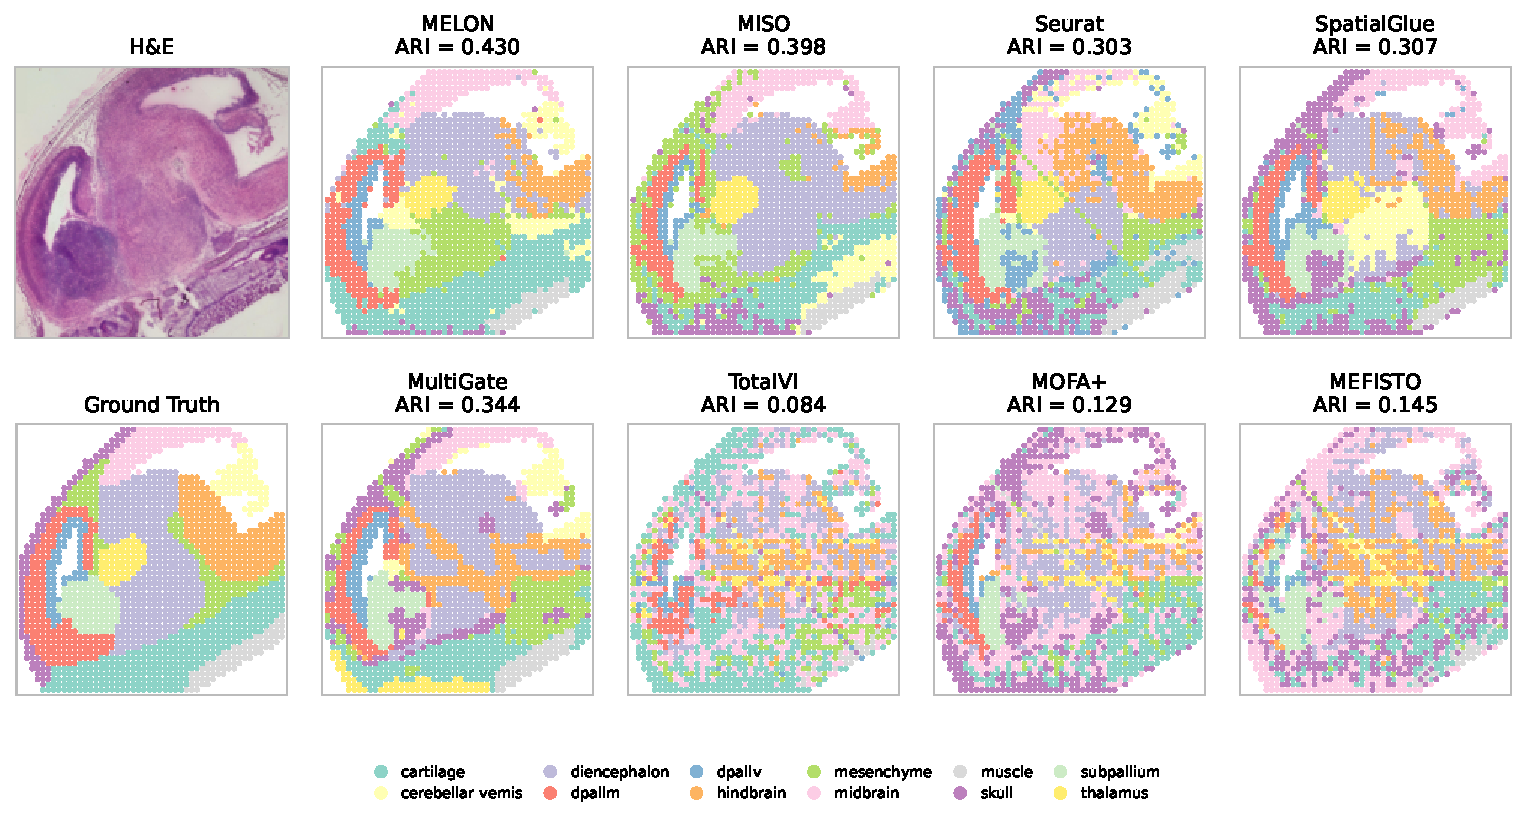
\includegraphics[width=\linewidth]{figures/mouse_E15_brain_panelC.pdf}
    \caption{H\&E image, ground-truth annotation, and spatial domain assignments from all eight benchmarked methods (ARI labelled per panel; methods ordered consistently across datasets).}
    \label{fig:dataset1_panel_c}
\end{subfigure}

\vspace{0.6ex}
\begin{subfigure}[b]{0.98\textwidth}
    \centering
    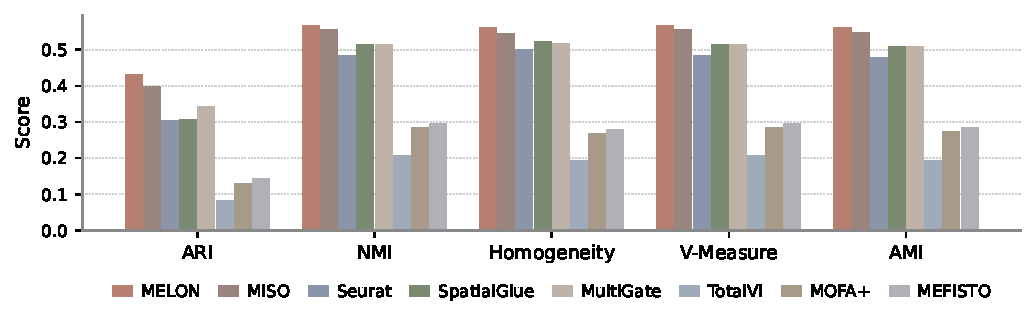
\includegraphics[width=0.90\linewidth]{figures/mouse_E15_brain_panelD.pdf}
    \caption{Clustering metrics (ARI, NMI, Homogeneity, V-Measure, AMI) across all eight methods at $k=12$.}
    \label{fig:dataset1_panel_d}
\end{subfigure}
\caption{Mouse E15.5 brain results. (a) H\&E tissue image, ground-truth annotation, and spatial domain assignments from MELON and seven multimodal baselines (per-panel ARI). (b) Five clustering metrics across all eight methods. Benchmark-over-$k$ curves are provided in Appendix~\ref{fig:app-dataset1-metrics}.}
\label{fig:dataset1_results}
\end{figure*}
\FloatBarrier

\textbf{Performance across datasets and metrics.}
Aggregating across the swept cluster numbers $k$ (median~$\pm$~IQR; Table~\ref{tab:multimethod_metrics}), MELON attains the best median on \emph{all 11 metrics} for the Mouse E15.5 brain (e.g., ARI $0.480 \pm 0.022$ vs.\ next-best MultiGate $0.344 \pm 0.025$); on \emph{9 of 11} for the Human lymph node (ARI $0.298 \pm 0.028$ vs.\ MISO $0.241 \pm 0.046$, with SpatialGlue narrowly leading homogeneity and MISO leading FMI); and on \emph{10 of 11} for the Mouse E13 embryo (ARI $0.385 \pm 0.007$ vs.\ SpatialGlue $0.280 \pm 0.014$, with Seurat winning only the internal-compactness CHI). Visually, MELON produces sharper anatomical boundaries and reduced cross-region mixing than every baseline---most clearly at the DPallm/DPallv, subpallium/thalamus, and midbrain/hindbrain interfaces in the brain (Fig.~\ref{fig:dataset1_panel_c}), the follicle/T-cell-zone and medulla/capsule interfaces in the lymph node (Appendix Fig.~\ref{fig:dataset2_panel_c}), and the neural/mesenchymal contacts in the embryo (Appendix Fig.~\ref{fig:dataset3_panel_c}).

\textbf{Robustness across $k$ and clustering backend.}
MELON's lead is stable across the swept cluster numbers: the per-method metric-versus-$k$ curves in Appendix Figs.~\ref{fig:app-dataset1-metrics}, \ref{fig:app-dataset2-metrics}, and~\ref{fig:app-dataset3-metrics} keep MELON at or near the top across the full $k$ range, with tighter IQR than every multimodal baseline. On the lymph node we further verified that swapping the downstream clustering backend on the frozen MELON embedding (GMM, Leiden, Louvain, Spectral, Walktrap) preserves the lead, and on the embryo we swept the spatial-graph neighborhood $k_{\mathrm{nn}}\in[4,11]$ with MELON remaining the top-performing approach throughout (Appendix~\ref{app:extra-exp}).

\begin{table}[H]
\centering
\caption{Clustering metrics across the three benchmarked datasets, aggregated across cluster numbers $k$ (median $\pm$ IQR; $k\in\{6,8,10,12,14\}$ for Mouse E15.5 Brain and Human Lymph Node, $k\in\{10,12,14,16,18\}$ for Mouse E13 Embryo). Best median per (dataset, metric) in \textbf{bold}. SpRI/SpARI: spatial Rand / adjusted Rand index; FMI: Fowlkes--Mallows; CHI: Calinski--Harabasz.}
\label{tab:multimethod_metrics}
\scriptsize
\setlength{\tabcolsep}{2.5pt}
\resizebox{\textwidth}{!}{%
\begin{tabular}{llccccccccccc}
\toprule
Dataset & Method & ARI & NMI & AMI & Homog. & V-Meas. & SpRI & SpARI & FMI & Jaccard & CHI & Purity \\
\midrule
\multirow{8}{*}{\textit{Mouse E15.5 Brain}} & \textbf{MELON} & $\mathbf{0.480 \pm 0.022}$ & $\mathbf{0.569 \pm 0.005}$ & $\mathbf{0.561 \pm 0.006}$ & $\mathbf{0.532 \pm 0.028}$ & $\mathbf{0.569 \pm 0.005}$ & $\mathbf{0.933 \pm 0.003}$ & $\mathbf{0.532 \pm 0.030}$ & $\mathbf{0.567 \pm 0.016}$ & $\mathbf{0.384 \pm 0.016}$ & $\mathbf{8927 \pm 2007}$ & $\mathbf{0.678 \pm 0.032}$ \\
 & MISO & $0.216 \pm 0.011$ & $0.372 \pm 0.027$ & $0.364 \pm 0.026$ & $0.355 \pm 0.046$ & $0.372 \pm 0.027$ & $0.888 \pm 0.004$ & $0.176 \pm 0.014$ & $0.324 \pm 0.007$ & $0.193 \pm 0.003$ & $156 \pm 28$ & $0.485 \pm 0.034$ \\
 & Seurat & $0.291 \pm 0.017$ & $0.483 \pm 0.007$ & $0.475 \pm 0.010$ & $0.491 \pm 0.041$ & $0.483 \pm 0.007$ & $0.905 \pm 0.003$ & $0.224 \pm 0.026$ & $0.376 \pm 0.016$ & $0.226 \pm 0.008$ & $3056 \pm 373$ & $0.560 \pm 0.041$ \\
 & SpatialGlue & $0.285 \pm 0.024$ & $0.515 \pm 0.019$ & $0.508 \pm 0.016$ & $0.524 \pm 0.063$ & $0.515 \pm 0.019$ & $0.904 \pm 0.006$ & $0.249 \pm 0.021$ & $0.381 \pm 0.026$ & $0.235 \pm 0.024$ & $212 \pm 17$ & $0.625 \pm 0.055$ \\
 & MultiGate & $0.344 \pm 0.025$ & $0.515 \pm 0.006$ & $0.508 \pm 0.004$ & $0.516 \pm 0.050$ & $0.515 \pm 0.006$ & $0.912 \pm 0.001$ & $0.321 \pm 0.110$ & $0.425 \pm 0.061$ & $0.270 \pm 0.038$ & $420 \pm 60$ & $0.596 \pm 0.027$ \\
 & TotalVI & $0.086 \pm 0.019$ & $0.212 \pm 0.059$ & $0.200 \pm 0.056$ & $0.199 \pm 0.068$ & $0.212 \pm 0.059$ & $0.860 \pm 0.011$ & $0.001 \pm 0.014$ & $0.211 \pm 0.001$ & $0.117 \pm 0.002$ & $409 \pm 101$ & $0.372 \pm 0.051$ \\
 & MOFA+ & $0.130 \pm 0.018$ & $0.300 \pm 0.017$ & $0.289 \pm 0.014$ & $0.273 \pm 0.033$ & $0.300 \pm 0.017$ & $0.869 \pm 0.006$ & $0.085 \pm 0.021$ & $0.265 \pm 0.024$ & $0.152 \pm 0.013$ & $631 \pm 13$ & $0.436 \pm 0.021$ \\
 & MEFISTO & $0.151 \pm 0.009$ & $0.301 \pm 0.018$ & $0.292 \pm 0.017$ & $0.281 \pm 0.031$ & $0.301 \pm 0.018$ & $0.873 \pm 0.004$ & $0.087 \pm 0.018$ & $0.269 \pm 0.019$ & $0.155 \pm 0.009$ & $530 \pm 29$ & $0.443 \pm 0.021$ \\
\midrule
\multirow{8}{*}{\textit{Human Lymph Node}} & \textbf{MELON} & $\mathbf{0.298 \pm 0.028}$ & $\mathbf{0.379 \pm 0.002}$ & $\mathbf{0.374 \pm 0.001}$ & $0.401 \pm 0.033$ & $\mathbf{0.379 \pm 0.002}$ & $\mathbf{0.858 \pm 0.004}$ & $\mathbf{0.307 \pm 0.038}$ & $0.454 \pm 0.018$ & $\mathbf{0.293 \pm 0.015}$ & $\mathbf{7265 \pm 576}$ & $\mathbf{0.643 \pm 0.009}$ \\
 & MISO & $0.241 \pm 0.046$ & $0.305 \pm 0.035$ & $0.301 \pm 0.032$ & $0.263 \pm 0.071$ & $0.305 \pm 0.035$ & $0.839 \pm 0.012$ & $0.281 \pm 0.017$ & $\mathbf{0.455 \pm 0.003}$ & $0.285 \pm 0.010$ & $241 \pm 47$ & $0.576 \pm 0.065$ \\
 & Seurat & $0.182 \pm 0.000$ & $0.260 \pm 0.006$ & $0.256 \pm 0.005$ & $0.236 \pm 0.017$ & $0.260 \pm 0.006$ & $0.824 \pm 0.000$ & $0.185 \pm 0.014$ & $0.389 \pm 0.018$ & $0.240 \pm 0.012$ & $597 \pm 126$ & $0.529 \pm 0.004$ \\
 & SpatialGlue & $0.227 \pm 0.049$ & $0.375 \pm 0.023$ & $0.371 \pm 0.024$ & $\mathbf{0.423 \pm 0.023}$ & $0.375 \pm 0.023$ & $0.837 \pm 0.012$ & $0.195 \pm 0.084$ & $0.371 \pm 0.065$ & $0.220 \pm 0.061$ & $375 \pm 51$ & $0.624 \pm 0.008$ \\
 & MultiGate & $0.148 \pm 0.011$ & $0.203 \pm 0.013$ & $0.199 \pm 0.012$ & $0.221 \pm 0.038$ & $0.203 \pm 0.013$ & $0.823 \pm 0.002$ & $0.147 \pm 0.017$ & $0.325 \pm 0.022$ & $0.192 \pm 0.019$ & $1289 \pm 133$ & $0.484 \pm 0.001$ \\
 & TotalVI & $0.181 \pm 0.006$ & $0.258 \pm 0.001$ & $0.253 \pm 0.000$ & $0.232 \pm 0.001$ & $0.258 \pm 0.001$ & $0.823 \pm 0.001$ & $0.187 \pm 0.011$ & $0.393 \pm 0.010$ & $0.242 \pm 0.007$ & $418 \pm 105$ & $0.525 \pm 0.004$ \\
 & MOFA+ & $0.212 \pm 0.032$ & $0.321 \pm 0.033$ & $0.318 \pm 0.031$ & $0.306 \pm 0.103$ & $0.321 \pm 0.033$ & $0.834 \pm 0.009$ & $0.229 \pm 0.025$ & $0.415 \pm 0.036$ & $0.261 \pm 0.020$ & $1042 \pm 81$ & $0.589 \pm 0.073$ \\
 & MEFISTO & $0.200 \pm 0.011$ & $0.307 \pm 0.007$ & $0.302 \pm 0.005$ & $0.310 \pm 0.045$ & $0.307 \pm 0.007$ & $0.832 \pm 0.002$ & $0.221 \pm 0.050$ & $0.400 \pm 0.044$ & $0.249 \pm 0.036$ & $854 \pm 82$ & $0.594 \pm 0.046$ \\
\midrule
\multirow{8}{*}{\textit{Mouse E13 Embryo}} & \textbf{MELON} & $\mathbf{0.385 \pm 0.007}$ & $\mathbf{0.528 \pm 0.010}$ & $\mathbf{0.519 \pm 0.007}$ & $\mathbf{0.546 \pm 0.039}$ & $\mathbf{0.528 \pm 0.010}$ & $\mathbf{0.925 \pm 0.001}$ & $\mathbf{0.362 \pm 0.026}$ & $\mathbf{0.452 \pm 0.022}$ & $\mathbf{0.290 \pm 0.023}$ & $191 \pm 40$ & $\mathbf{0.655 \pm 0.008}$ \\
 & MISO & $0.227 \pm 0.014$ & $0.441 \pm 0.031$ & $0.431 \pm 0.028$ & $0.417 \pm 0.046$ & $0.441 \pm 0.031$ & $0.899 \pm 0.004$ & $0.251 \pm 0.005$ & $0.337 \pm 0.002$ & $0.197 \pm 0.002$ & $204 \pm 29$ & $0.521 \pm 0.053$ \\
 & Seurat & $0.266 \pm 0.043$ & $0.454 \pm 0.017$ & $0.443 \pm 0.020$ & $0.487 \pm 0.017$ & $0.454 \pm 0.017$ & $0.910 \pm 0.002$ & $0.223 \pm 0.073$ & $0.341 \pm 0.047$ & $0.201 \pm 0.041$ & $\mathbf{5180 \pm 318}$ & $0.571 \pm 0.005$ \\
 & SpatialGlue & $0.280 \pm 0.014$ & $0.460 \pm 0.022$ & $0.451 \pm 0.018$ & $0.472 \pm 0.063$ & $0.460 \pm 0.022$ & $0.910 \pm 0.001$ & $0.238 \pm 0.043$ & $0.355 \pm 0.018$ & $0.215 \pm 0.016$ & $306 \pm 35$ & $0.600 \pm 0.061$ \\
 & MultiGate & $0.170 \pm 0.016$ & $0.380 \pm 0.008$ & $0.369 \pm 0.007$ & $0.392 \pm 0.031$ & $0.380 \pm 0.008$ & $0.899 \pm 0.003$ & $0.168 \pm 0.056$ & $0.263 \pm 0.036$ & $0.151 \pm 0.025$ & $1342 \pm 133$ & $0.438 \pm 0.021$ \\
 & TotalVI & $0.092 \pm 0.003$ & $0.224 \pm 0.033$ & $0.212 \pm 0.029$ & $0.164 \pm 0.030$ & $0.224 \pm 0.033$ & $0.819 \pm 0.002$ & $0.140 \pm 0.005$ & $0.321 \pm 0.000$ & $0.149 \pm 0.000$ & $195 \pm 22$ & $0.307 \pm 0.006$ \\
 & MOFA+ & $0.201 \pm 0.012$ & $0.389 \pm 0.012$ & $0.377 \pm 0.009$ & $0.383 \pm 0.040$ & $0.389 \pm 0.012$ & $0.897 \pm 0.008$ & $0.199 \pm 0.033$ & $0.295 \pm 0.017$ & $0.173 \pm 0.010$ & $1203 \pm 49$ & $0.491 \pm 0.030$ \\
 & MEFISTO & $0.207 \pm 0.015$ & $0.391 \pm 0.003$ & $0.381 \pm 0.007$ & $0.392 \pm 0.018$ & $0.391 \pm 0.003$ & $0.900 \pm 0.003$ & $0.189 \pm 0.050$ & $0.302 \pm 0.032$ & $0.178 \pm 0.021$ & $767 \pm 29$ & $0.496 \pm 0.017$ \\
\bottomrule
\end{tabular}}
\end{table}

\subsubsection{Interpretability via a Joint Pair Decoder}
To probe whether MELON's frozen embedding admits a biologically meaningful joint factorisation~\cite{doshivelez2017rigorous,rudin2019stop}, we train a small \emph{pair decoder} on top of the frozen fused embedding $\mathbf{z}_i$ for each of the three datasets. This follows the post-hoc probing paradigm for interpreting frozen representations~\cite{alain2017probes}, instantiated as a post-hoc concept-bottleneck decoder~\cite{koh2020concept,yuksekgonul2023pcbm,svensson2020ldvae} in which each latent factor is directly read out as a gene/peak program. The decoder is a two-headed MLP with a non-negative factor bottleneck $\mathbf{u}_i = \mathrm{softplus}(\phi(\mathbf{z}_i)) \in \mathbb{R}_{\geq 0}^{K}$ (non-negativity promotes parts-based, additive programs as in NMF~\cite{lee1999nmf}) ($K{=}24$ for the two RNA--ATAC datasets, $K{=}16$ for the RNA--ADT lymph node) and two linear heads that simultaneously reconstruct the two modalities under a coupled loss
\begin{equation}\label{eq:pair-decoder-main}
    \mathcal{L}_{\text{dec}}
    \;=\;
    \tfrac{1}{N}\sum_{i=1}^{N}\Bigl[
        \bigl\|\mathbf{x}^{R}_i - \mathbf{W}^{R}\mathbf{u}_i\bigr\|_{2}^{2}
        \;+\;
        \mathrm{BCE}\!\bigl(\mathbf{x}^{A}_i,\,\sigma(\mathbf{W}^{A}\mathbf{u}_i)\bigr)
    \Bigr],
\end{equation}
where $\mathbf{W}^{R}$ and $\mathbf{W}^{A}$ are the gene and peak/protein loading matrices and $\sigma$ is the elementwise sigmoid; only the decoder is trained, MELON itself is frozen. Each latent factor $k$ is then summarised by its spatial usage $\{u_{i,k}\}_i$ together with its top gene--peak pair $(g^{\dagger}_k,p^{\dagger}_k) = \arg\max_{g,p}\,W^{R}_{g,k}W^{A}_{p,k}$ (full derivation in Appendix~\ref{app:interpretability}). Across datasets, factor usage is spatially compartmentalised and the top-ranked features include known developmental and immune markers (Cdh19~\cite{simoes2015neural}, Pou3f1~\cite{zhu2014pou3f1}, Prdm8~\cite{ross2012prdm8}, Uncx~\cite{mansouri1997uncx}, Ednrb~\cite{baynash1994ednrb}, FCGR3A/CD16~\cite{bruhns2012fcgr}, CD274/PD-L1~\cite{dong1999pdl1}, SDC1/CD138~\cite{wijdenes1996cd138}, PAX5~\cite{nutt1999pax5}), indicating that the embedding preserves localised cross-modal programs beyond what clustering alone reveals. Per-dataset factor usage maps and curated top gene--peak spatial maps are reported in Appendix~\ref{app:interpretability}.

Additional sensitivity analyses, interpretability results, and qualitative case studies are deferred to Appendix~\ref{app:extra-exp} to keep the main paper within the NeurIPS page limit.

\section{Conclusion}
We presented \melon{}, a spatial multimodal representation-learning framework that combines modality-specific encoding, neighborhood-aware spatial attention, transformer-based fusion, and a PID-guided contrastive objective. Across paired RNA--ATAC and RNA--ADT datasets, MELON produced spatially coherent domains and improved agreement with anatomical annotations relative to strong multimodal baselines. These results suggest that preserving shared, modality-specific, and synergistic information is important for accurate spatial multi-omics integration and domain identification. More broadly, the results support a perspective on spatial multi-omics integration in which complementary structure across assays should be modeled explicitly rather than compressed into a purely shared latent space. A practical next step is to extend MELON to additional modality combinations and larger tissue collections, where richer cross-modal interactions may further improve domain discovery and biological interpretation.

\section*{Acknowledgments}
% TODO: add funding sources and acknowledgments here before arXiv upload.

\bibliographystyle{plainnat}
\bibliography{ref}

%%%%%%%%%%%%%%%%%%%%%%%%%%%%%%%%%%%%%%%%%%%%%%%%%%%%%%%%%%%%
\newpage
\appendix
\onecolumn

\section{Related Work}\label{app:related_work}

This section expands the brief related-work summary in the main text into a fuller discussion organized by sub-topic.

\paragraph{Spatial Multi-Omics Integration.}
A central challenge in spatial multi-omics is learning a unified embedding from heterogeneous modalities (e.g., RNA expression and chromatin accessibility) while preserving the spatial organization of tissue. Early approaches adapted single-cell integration tools to the spatial setting. Seurat~\cite{hao2021seurat} performs anchor-based canonical correlation analysis followed by graph-based clustering, but treats spots as independent observations and discards spatial coordinates. MOFA+~\cite{argelaguet2020mofa} extends multi-omics factor analysis with group and modality structure, yet the underlying linear factor model cannot capture non-linear cross-modal interactions and has no mechanism to incorporate spatial information. TotalVI~\cite{gayoso2021totalvi} jointly models RNA and protein (CITE-seq) counts via a variational autoencoder (VAE), but likewise assumes i.i.d.\ cells and does not exploit spatial neighborhoods. MultiVI~\cite{ashuach2023multivi} extends the VAE paradigm to handle partially observed modalities; however, it still lacks spatial awareness and relies on largely linear/Gaussian priors. MEFISTO~\cite{velten2022mefisto} introduces Gaussian-process priors over a spatial or temporal axis to encourage smooth latent factors, effectively capturing spatially coherent variation, but its reconstruction-based objective emphasizes shared (redundant) variation and can over-smooth domain boundaries. SpatialGlue~\cite{long2024spatialglue} couples graph convolutional networks with a VAE, building a spatial neighbor graph per modality and fusing representations via cross-attention. While SpatialGlue explicitly models spatial structure, its reconstruction loss still primarily captures redundancy and can average away sharp boundaries. In contrast, MELON uses a contrastive objective that captures not only shared (redundant) information but also unique and synergistic cross-modal signals, combined with a learned spatial attention bias that preserves tissue boundaries.

\paragraph{Contrastive Representation Learning.}
Contrastive self-supervised methods learn representations by pulling positive pairs together and pushing negative pairs apart in an embedding space. The InfoNCE estimator was introduced by~\citet{oord2018representation} and popularised for image self-supervised learning by SimCLR~\cite{chen2020simple}, which showed that data-augmentation-based positive pairs, a projection head, and large batch sizes are critical for performance. \citet{tian2020contrastive} (Contrastive Multiview Coding, CMC) extended InfoNCE to multiple augmentations of the same scene, providing the multi-modality contrastive paradigm that subsequent multimodal methods build on. CLIP~\cite{radford2021learning} applied a two-modality symmetric cross-modal InfoNCE loss to image--text pairs at scale. The theoretical foundations of which information these losses recover trace back to \emph{partial information decomposition} (PID,~\citet{williams2010nonnegative,bertschinger2014quantifying}), which decomposes the joint mutual information $I(X_1, X_2; Y)$ into redundancy ($R$), modality-specific uniqueness ($U_1, U_2$), and synergy ($S$). Building on these two threads, the CoMM framework~\cite{dufumier2024align} showed that standard CLIP-style two-modality objectives capture only $R$, and proposed a modality-masking InfoNCE loss whose terms provably (Lemmas 2 and 3) align with all four PID components, including $S$. MELON directly builds on this framework: it generates modality-masked and joint embeddings and contrasts each modality-masked embedding against the joint embedding, ensuring that the learned embedding captures all four information components.

\paragraph{Spatial Inductive Biases for Transcriptomics.}
Incorporating spatial structure into representation learning for spatially resolved data is a well-studied problem with two broad families of approaches: graph neural networks that perform explicit message passing, and attention-bias methods that modulate Transformer attention with positional priors.

On the GNN side, Graph Attention Networks (GAT)~\cite{velivckovic2018gat} learn adaptive edge weights via $\mathrm{LeakyReLU}(\mathbf{a}^\top [W\mathbf{h}_i \,\|\, W\mathbf{h}_j])$ and \emph{aggregate} neighbour features through a weighted sum, producing new node embeddings at each layer. In spatial transcriptomics, STAGATE~\cite{dong2022deciphering} applies a graph attention autoencoder over a spatial neighbor graph for spatial domain identification, and GraphST~\cite{long2023spatially} combines graph contrastive learning with spatial neighbor aggregation. SpaceFlow~\cite{ren2022spaceflow} uses a spatially regularised deep graph network to learn pseudo-spatiotemporal embeddings. These methods perform true message passing---each node's representation is updated by aggregating information from its neighbours---but are designed for a single modality (gene expression).

On the attention-bias side, recent work in NLP and vision has shown that injecting learned or fixed positional biases directly into Transformer attention scores is an effective alternative to explicit positional encodings. ALiBi~\cite{press2022train} adds a linear distance penalty to attention logits, and relative position biases~\cite{raffel2020exploring,shaw2018self} parameterise position-dependent offsets in the attention matrix.

MELON's spatial module (internally called \emph{NeighborhoodGAT}) falls squarely in the second category: it is \textbf{not} a standard GAT despite the name. It computes a learned attention bias over a $k$-nearest-neighbour graph from positional embeddings of the spot coordinates $u_i = \psi(s_i)$, using an additive GAT-style edge logit $\mathrm{LeakyReLU}(a_{\mathrm{src}}^{(h)\top} h_i^{(h)} + a_{\mathrm{dst}}^{(h)\top} h_j^{(h)})$ with per-head learned vectors $a_{\mathrm{src}}^{(h)}, a_{\mathrm{dst}}^{(h)}$ and projections $h_i^{(h)} = W^{(h)} u_i$ (Methods \S\ref{subsec:neighgat}), but critically performs \textbf{no message passing and no neighbour-feature aggregation}. Instead, the module outputs a log-space bias matrix $B \in \mathbb{R}^{N \times N}$ that is injected additively into the Transformer's scaled dot-product attention: $\mathrm{softmax}(QK^\top/\sqrt{d_k} + B)V$. Because the bias is additive in log-space, it is equivalent to \emph{multiplicatively gating} content-based attention by learned spatial proximity weights, with non-neighbour entries receiving $\log\epsilon \approx -13.8$ and therefore effectively zero attention. This design is modality-invariant---the same spatial bias is block-tiled and applied regardless of which modality combination is active under the masking strategy (Appendix~\ref{app:impl-bias})---and integrates seamlessly with the Transformer's Grouped Query Attention (GQA)~\cite{ainslie2023gqa}.

\section{Datasets and Preprocessing}\label{app:datasets}

We evaluate MELON on three paired spatial multimodal datasets that span embryonic brain, embryonic whole-embryo, and human lymphoid tissue settings. Together they cover both RNA--ATAC and RNA--protein integration, different tissue architectures, and a range of spatial domain granularities.

\begin{table}[!ht]
\centering
\caption{Dataset statistics used in experiments. For ATAC modalities, the raw peak matrices are reduced to $50$ components via TF--IDF + LSI before modeling (Appendix~\ref{app:impl-aug}).}
\label{tab:dataset-stats}
\small
\begin{tabular}{lcccc}
\toprule
Dataset & \#Spots & Modality 1 & Modality 2 & \#Domains \\
\midrule
Mouse E15.5 Brain & 1{,}949 & 2{,}144 genes & 47{,}287 peaks & 12 \\
Mouse E13 Embryo & 2{,}187 & 17{,}058 genes & 24{,}017 peaks & 14 \\
Human Lymph Node & 3{,}484 & 18{,}085 genes & 31 proteins & 10 \\
\bottomrule
\end{tabular}
\end{table}

\paragraph{Mouse E15.5 Brain (MISAR-seq).}
This dataset profiles an embryonic day 15.5 mouse brain sagittal section using MISAR-seq (Microfluidic Indexing-based Spatial ATAC and RNA-seq), which simultaneously measures chromatin accessibility and gene expression at 50\,$\mu$m grid resolution ($\sim$15--30 cells per spot)~\cite{zuo2023misar}. The dataset contains 1{,}949 spots with 2{,}144 RNA features and 47{,}287 ATAC peaks. Ground-truth labels comprise 12 manually annotated neuroanatomical regions (diencephalon, cartilage, hindbrain, dorsal pallium medial/ventral, mesenchyme, midbrain, skull, subpallium, muscle, cerebellar vermis, thalamus), validated against the Allen Mouse Brain Atlas. RNA counts are normalized with \texttt{normalize\_total} (target sum $10^4$) followed by $\log(1+x)$. ATAC peaks are transformed via TF--IDF weighting followed by Latent Semantic Indexing (truncated SVD with $50$ components), yielding a 50-dimensional input per spot. Data are publicly available at GEO accession \texttt{GSE213264}.

\paragraph{Human Lymph Node (Visium RNA--ADT).}
This dataset profiles two sequential 5\,$\mu$m FFPE sections of a human lymph node using the 10x Genomics Visium CytAssist platform~\cite{long2024spatialglue}. Sections were stained with H\&E following the CytAssist FFPE protocol (CG000658, 10x Genomics) including deparaffinization, staining, imaging, and decrosslinking, with imaging on an EVOS M7000 microscope ($\times$20 objective). Spatial gene expression libraries were prepared with the Visium Human Transcriptome Probe Set v2.0 and spatial protein expression libraries with the Human FFPE Immune Profiling Panel (31 antibody targets + 4 isotype controls = 35-plex; antibodies from BioLegend and Abcam, signals normalized to isotype controls). Libraries were sequenced on an Illumina NovaSeq S2 PE50 ($\sim$2{,}000\,M reads per lane) and processed with Space Ranger v2.1.0 against GRCh38 (GENCODE v32 / Ensembl 98). The dataset contains 3{,}484 spots with 18{,}085 genes and 31 proteins. Reference labels comprise 10 manually annotated lymphoid compartments (medulla cords, medulla sinuses, cortex, pericapsular adipose tissue, capsule, subcapsular sinus, follicle, medulla vessels, hilum, trabeculae) curated from H\&E images in Loupe Browser. RNA counts are $\log(1+x)$-normalized; ADT counts are transformed via centered log-ratio (CLR) normalization. Data are available at \url{https://zenodo.org/records/10362607}.

\paragraph{Mouse E13 Embryo (spatial-ATAC--RNA-seq).}
This dataset profiles a whole embryonic day 13 mouse section with paired RNA and ATAC (H3K27ac active chromatin marks) using spatial-ATAC--RNA-seq, which co-profiles the epigenome and transcriptome at 50\,$\mu$m pixel resolution via deterministic barcoding in tissue (DBiT-seq)~\cite{zhang2023spatial}. It contains 2{,}187 spatial locations, 17{,}058 genes, and 24{,}017 ATAC peaks. Ground-truth annotations comprise 14 embryonic regions (ventral trunk, surface ectoderm, forebrain, paraxial mesoderm, dorsal head/body-wall mesenchyme, periventricular neuroepithelium, spinal cord, head mesenchyme, caudal ventral trunk, gut/ventral endoderm, hindbrain--cervical transition, trunk mesenchyme, eye, visceral organ primordia). Preprocessing follows the same recipe as the E15.5 dataset: $\log(1+x)$ for RNA and TF--IDF + LSI ($50$ components) for ATAC. This benchmark complements the E15.5 brain dataset by testing MELON on a larger developmental system with broader anatomical diversity.

\section{Implementation Details}\label{app:impl}

\subsection{Preprocessing and Augmentations}\label{app:impl-aug}

MELON operates on modality-specific input matrices after standard preprocessing for each assay. The framework is agnostic to the choice of preprocessing -- continuous, normalized, or low-rank-reduced features all work as drop-in inputs to the per-modality encoder $f_m$ -- and the concrete recipes used for the assays in our experiments (RNA, ATAC, ADT) are described in Appendix~\ref{app:datasets}. During training, augmentations are applied before the encoder so that the model never observes a clean batch in the contrastive forward pass.

For each batch, MELON samples two independent augmented multimodal inputs by independently applying three stochastic transformations: Gaussian noise, feature dropout, and aligned cross-spot mixing (the latter shares its permutation and mixing coefficient across all modalities of the same spot so that cross-modal correspondences are preserved). The functional form of each augmentation and the exact hyperparameters used in our experiments ($\sigma$, dropout fraction, mixing distribution, and activation probability) are listed in Appendix~\ref{app:impl-hparams}.

\subsection{Spot Tokenization and Token Recovery}\label{app:impl-token}

Let $N$ denote the batch size and $n$ the number of modalities ($n = 2$ in all of our experiments). After the modality-specific encoders and token-space projection, MELON has one embedding per spot and per modality. With spot tokenization enabled, the batch dimension is reinterpreted as the token dimension, so that each modality contributes a length-$N$ token sequence:
\begin{equation}
  T^{(m)} \in \mathbb{R}^{1 \times N \times d}, \qquad m \in \{1, \ldots, n\}.
\end{equation}
Concatenating modalities yields a single token sequence
\begin{equation}
  T = \mathrm{concat}\bigl(T^{(1)}, \ldots, T^{(n)}\bigr) \in \mathbb{R}^{1 \times (nN) \times d}.
\end{equation}
Thus, token $i$ corresponds to spot $i$ in modality $1$, token $N+i$ to the same spot in modality $2$, and so on. The transformer therefore attends jointly across all spot--modality pairs in the batch.

After the fusion transformer outputs all active tokens, the resulting tensor is reshaped back into modality-by-spot blocks and pooled across modalities to recover one fused embedding per spot:
\begin{equation}
  \tilde{T} \in \mathbb{R}^{1 \times (nN) \times d}
  \rightarrow
  \mathbb{R}^{n \times N \times d},
  \qquad
  z_i = \frac{1}{n}\sum_{m=1}^{n} \tilde{t}^{(m)}_i.
\end{equation}
This tokenization scheme is the default because it allows the transformer to model both cross-modal and cross-spot interactions within a single attention layer.

\subsection{Spatial Bias Tiling and Modality Masking}\label{app:impl-bias}

NeighborhoodGAT produces a spot-level spatial bias matrix $B \in \mathbb{R}^{N \times N}$, where $N$ is the batch size as defined in Appendix~\ref{app:impl-token}. Under spot tokenization, however, the transformer sees $nN$ tokens rather than $N$ spots. To align the spatial prior with the token layout, we tile the spot-level bias across modality blocks into the matrix $B_{\mathrm{spatial}}$ used in the fusion-transformer attention (\S\ref{subsec:fusion-transformer}). For $n$ modalities, $B_{\mathrm{spatial}}$ is an $n \times n$ block matrix in which every block equals $B$; we write the $n=2$ case explicitly here for concreteness:
\begin{equation}
  B_{\mathrm{spatial}} =
  \begin{bmatrix}
    B & B \\
    B & B
  \end{bmatrix}
  \in \mathbb{R}^{2N \times 2N}.
\end{equation}
This tiling enforces that the spatial relationship between spot $i$ and spot $j$ is modality-invariant: the same bias is used whether attention connects within-modality token pairs (modality $m$ to modality $m$) or cross-modal token pairs (modality $m$ to modality $m'$) for those two spots. For $n$ modalities the construction generalises by replacing the $2 \times 2$ block matrix above with an $n \times n$ block matrix whose every block is $B$.

MELON then evaluates the fusion module under $n + 1$ modality masks: $n$ single-modality passes and one joint multimodal pass. When only modality $m$ is active, the token sequence is physically subsetted and the tiled bias is sliced to the diagonal block corresponding to $m$, which by construction equals the underlying spot-level bias $B$. For the multimodal pass, the full tiled matrix is used. This design guarantees that single-modality and multimodal forward passes share the same underlying spot-level spatial bias.

\subsection{Hyperparameters}\label{app:impl-hparams}

MELON is implemented in PyTorch with PyTorch Lightning. All defaults used in this paper are listed in Table~\ref{tab:hyperparams} and were not tuned per dataset. Augmentation functional forms are described in \S\ref{subsec:augmentations}; the values in the table refer to the parameters of those functions. After training, the joint embedding is clustered with Leiden clustering; the implementation also supports Louvain, Walktrap, spectral, and GMM for downstream exploration.

\begin{table}[!htbp]
\centering
\caption{MELON default hyperparameters. All values were used as-is across the three benchmarked datasets without per-dataset tuning.}
\label{tab:hyperparams}
\small
\begin{tabular}{lll}
\toprule
Group & Hyperparameter & Value \\
\midrule
\multirow{4}{*}{Encoder}
  & Per-modality encoder      & 2-layer MLP, $d_m \!\rightarrow\! 128 \!\rightarrow\! 128$, ReLU \\
  & Embedding dimension       & $128$ \\
  & Projection head           & 3-layer MLP, $128\!\rightarrow\!256\!\rightarrow\!256\!\rightarrow\!128$, SyncBatchNorm \\
  & Output normalisation      & L2 \\
\midrule
\multirow{4}{*}{Fusion transformer}
  & Layers                    & $1$ \\
  & Attention                 & Grouped Query Attention, $8$ heads \\
  & MLP expansion / activation& $4\times$ / QuickGELU \\
  & Spatial bias              & additive (NeighborhoodGAT, see below) \\
\midrule
\multirow{5}{*}{NeighborhoodGAT}
  & Layers / heads            & $1$ / $8$ \\
  & Hidden dim per head       & $64$ \\
  & Attention dropout         & $0.1$ \\
  & LeakyReLU slope           & $0.2$ \\
  & Spatial $k$-NN graph      & $k=16$, self-loops included \\
\midrule
\multirow{6}{*}{Optimisation}
  & Optimiser                 & Adam, $(\beta_1,\beta_2)=(0.9,0.999)$ \\
  & Learning rate             & $1\!\times\!10^{-3}$ \\
  & Weight decay              & $1\!\times\!10^{-5}$ \\
  & Schedule                  & none \\
  & Epochs                    & $100$ \\
  & Batch size                & $2{,}048$ \\
\midrule
\multirow{2}{*}{Loss}
  & Temperature $\tau$        & $0.1$ \\
  & Per-mask weighting        & equal across $n{+}1$ masks (Eq.~\ref{eq:melon-loss}) \\
\midrule
\multirow{4}{*}{Augmentations}
  & Activation probability    & $p=0.8$ per augmentation \\
  & Gaussian noise            & $\sigma=0.05$ \\
  & Feature dropout           & fraction $0.2$ \\
  & Neighbour mix             & $\lambda\sim\mathrm{Beta}(0.3,0.3)$, shared $\pi,\lambda$ across modalities \\
\midrule
\multirow{3}{*}{Reproducibility}
  & Random seed               & $42$ (PyTorch, NumPy, Python \texttt{random}) \\
  & Hardware                  & CPU (Apple Silicon / MPS) or single CUDA GPU \\
  & Framework                 & PyTorch + PyTorch Lightning \\
\bottomrule
\end{tabular}
\end{table}

\FloatBarrier
\section{Proof of Proposition~\ref{prop:pid-inheritance}}\label{app:proof}

\begin{proposition}[PID inheritance under spatial bias]\label{prop:pid-inheritance}
Let $f_\theta$ be an encoder satisfying the standard expressivity assumption (Assumption~\ref{ass:expressivity}), and let $B$ be any spatial-bias matrix injected as an additive term in $f_\theta$'s attention scores (\S\ref{subsec:neighgat}--\S\ref{subsec:fusion-transformer}). Suppose the augmentation family $\mathcal{T}$ used to draw the two augmented inputs $X', X''$ is label-preserving with respect to the latent spatial-domain identity $Y$ (Eq.~\ref{eq:assumption1}). Then at the supremum $\mathcal{L}_{\mathrm{MELON}}$ decomposes across the four PID quantities $\{R, S, U_1, \ldots, U_n\}$ through its joint and modality-masked terms: the joint term $\mathcal{L}_{\star}$ aligns the joint embedding with $R + S + \sum_{m=1}^{n} U_m$, each modality-masked term $\mathcal{L}_{m}$ aligns the modality-$m$ embedding with $R + U_m$, and each individual PID component is therefore identifiable from linear combinations of these loss-term optima.
\end{proposition}

\paragraph{Setup.} Let $X = (X^{(1)}, \ldots, X^{(n)})$ be a multimodal input, $Y$ a latent task variable, and $f_\theta : \mathcal{X} \to \mathcal{Z}$ an encoder. Let $\mathcal{T}^\star$ be a label-preserving augmentation family in the sense of~\citet{tian2020what}: two independent views $t'(X), t''(X)$ drawn from $\mathcal{T}^\star$ are jointly sufficient and minimal for $Y$, equivalently
\begin{equation}\label{eq:assumption1}
  \forall\, t', t'' \in \mathcal{T}^\star, \qquad I\bigl(t'(X),\, t''(X)\bigr) \;=\; I(X,\, Y).
\end{equation}
For $t', t'' \sim \mathcal{T}^\star$, write $X' = t'(X)$, $X'' = t''(X)$, and let
\begin{equation}\label{eq:joint-and-masked-encodings}
  Z'_{\theta} \;=\; f_\theta(X'),
  \qquad
  Z''_{\theta} \;=\; f_\theta(X''),
  \qquad
  Z^{[m]}_{\theta} \;=\; f_\theta\bigl(X^{[m]}\bigr),
\end{equation}
where $X^{[m]} = ([\mathrm{MSK}], \ldots, X^{(m)}, \ldots, [\mathrm{MSK}])$ is the modality-$m$-only masked input. The partial information decomposition~\citep{williams2010nonnegative,bertschinger2014quantifying} writes
\begin{equation}\label{eq:pid}
  I\bigl(X^{(1)}, \ldots, X^{(n)};\, Y\bigr) \;=\; R + S + \sum_{m=1}^{n} U_m,
\end{equation}
and the chain rule of mutual information gives the consistency relations~\citep{bertschinger2014quantifying}
\begin{equation}\label{eq:pid-consistency}
  I\bigl(X^{(m)}; Y\bigr) \;=\; R + U_m, \qquad m = 1, \ldots, n.
\end{equation}

\begin{assumption}[Expressivity of $f_\theta$]\label{ass:expressivity}
The encoder family $\{f_\theta\}_\theta$ is sufficiently rich that $\sup_\theta I(f_\theta(V); W) = I(V; W)$ for every pair of random variables $(V, W)$ appearing in the proof; equivalently, the supremum is attained by an $f_\theta$ that is a sufficient statistic of $V$ for $W$. (We use $V, W$ as generic placeholders to avoid clash with the spatial-bias matrix $B$.) This is the standard expressivity hypothesis used in neural mutual-information estimation~\citep{oord2018representation,tian2020contrastive}.
\end{assumption}

\paragraph{Proof.}
Recall the MELON loss from Eq.~\ref{eq:melon-loss},
\begin{equation}\label{eq:melon-loss-restate}
  \mathcal{L}_{\mathrm{MELON}}
  \;=\; \frac{1}{n+1}\Bigl(\mathcal{L}_{\star} \;+\; \sum_{m=1}^{n} \mathcal{L}_{m}\Bigr),
\end{equation}
with the joint and modality-masked per-mask terms (Eq.~\ref{eq:melon-perk})
\begin{align}
  \mathcal{L}_{\star}
    &\;=\; -\tfrac{1}{2}\Bigl(\widehat{I}_{\mathrm{NCE}}\bigl(Z'^{[\star]}_\theta,\, Z''^{[\star]}_\theta\bigr) + \widehat{I}_{\mathrm{NCE}}\bigl(Z''^{[\star]}_\theta,\, Z'^{[\star]}_\theta\bigr)\Bigr),
    \label{eq:lstar}\\[2pt]
  \mathcal{L}_{m}
    &\;=\; -\tfrac{1}{2}\Bigl(\widehat{I}_{\mathrm{NCE}}\bigl(Z'^{[m]}_\theta,\, Z''^{[\star]}_\theta\bigr) + \widehat{I}_{\mathrm{NCE}}\bigl(Z''^{[m]}_\theta,\, Z'^{[\star]}_\theta\bigr)\Bigr),
    \label{eq:lm}
\end{align}
where $Z'^{[\star]}_\theta = Z'_\theta$ and $Z''^{[\star]}_\theta = Z''_\theta$ denote the joint-mask embeddings.

\textbf{Step 1: $\mathcal{L}_{\star}$ recovers $R + S + \sum_m U_m$.}
Consider the Markov chains $X \to X' \to Z'_\theta$ and $X \to X'' \to Z''_\theta$, with $X'$ and $X''$ conditionally independent given $X$. Then
\begin{equation}\label{eq:step1-chain}
\begin{aligned}
\sup_{\theta} \bigl(-\mathcal{L}_{\star}\bigr)
  \;&=\; \sup_{\theta}\, \widehat{I}_{\mathrm{NCE}}\bigl(Z'_\theta,\, Z''_\theta\bigr)
    && \text{[Eq.~\eqref{eq:lstar}, symmetrisation]} \\
  \;&=\; \sup_{\theta}\, I\bigl(Z'_\theta,\, Z''_\theta\bigr)
    && \text{[\citealp{oord2018representation}, Assumption~\ref{ass:expressivity}]} \\
  \;&=\; I(X', X'')
    && \text{[data processing inequality, Assumption~\ref{ass:expressivity}]} \\
  \;&=\; I(X, Y)
    && \text{[label-preservation, Eq.~\eqref{eq:assumption1}]} \\
  \;&=\; R + S + \sum_{m=1}^{n} U_m
    && \text{[PID, Eq.~\eqref{eq:pid}]}.
\end{aligned}
\end{equation}
This follows the standard InfoNCE--mutual-information equivalence~\citep{oord2018representation} combined with the PID decomposition~\eqref{eq:pid}.

\textbf{Step 2: $\mathcal{L}_{m}$ recovers $R + U_m$ for each $m$.}
Consider the Markov chain $Y \to X^{(m)} \to X^{[m]} \to Z^{[m]}_\theta$, since the masked input $X^{[m]} = ([\mathrm{MSK}], \ldots, X^{(m)}, \ldots, [\mathrm{MSK}])$ depends on $X^{(m)}$ alone. Then
\begin{equation}\label{eq:step2-chain}
\begin{aligned}
\sup_{\theta} \bigl(-\mathcal{L}_{m}\bigr)
  \;&=\; \sup_{\theta}\, \widehat{I}_{\mathrm{NCE}}\bigl(Z^{[m]}_\theta,\, Z_\theta\bigr)
    && \text{[Eq.~\eqref{eq:lm}, symmetrisation]} \\
  \;&=\; \sup_{\theta}\, I\bigl(Z^{[m]}_\theta;\, Z_\theta\bigr)
    && \text{[\citealp{oord2018representation}, Assumption~\ref{ass:expressivity}]} \\
  \;&=\; \sup_{\theta}\, I\bigl(Z^{[m]}_\theta;\, Y\bigr)
    && \text{[Step 1: at the supremum $Z_\theta$ is a sufficient statistic of $Y$]} \\
  \;&=\; I\bigl(X^{(m)};\, Y\bigr)
    && \text{[data processing inequality, Assumption~\ref{ass:expressivity}]} \\
  \;&=\; R + U_m
    && \text{[PID consistency, Eq.~\eqref{eq:pid-consistency}]}.
\end{aligned}
\end{equation}
Note that this chain does not invoke the label-preservation hypothesis~\eqref{eq:assumption1}; the symmetric augmentation in MELON ($Z'^{[m]}_\theta, Z''^{[m]}_\theta$ both deterministic functions of $X^{(m)}$ via $t \in \mathcal{T}^\star$) leaves it unaffected, since the masked input depends on modality $m$ alone regardless of the augmentation applied.

\textbf{Step 3: the spatial bias preserves both chains.}
The bias $B$ enters $f_\theta$ only as an additive term in the attention logits, $\mathrm{Attn}(Q, K, V) = \mathrm{softmax}\bigl(QK^\top/\sqrt{d_k} + B\bigr)V$, and $B$ is computed solely from the spatial coordinates $S$ via NeighborhoodGAT (\S\ref{subsec:neighgat}), independently of the per-modality features $X^{(1)}, \ldots, X^{(n)}$. Conditioned on $S$, the bias $B$ is therefore a fixed observed covariate and $f_\theta(\,\cdot\,;\, B)$ is a deterministic function of $X$. The Markov chains of Steps~1 and~2 hold conditionally on $S$, so the chains~\eqref{eq:step1-chain} and~\eqref{eq:step2-chain} carry through under $f_\theta \mapsto f_\theta(\,\cdot\,;\, B)$.

\textbf{Conclusion.} Substituting Steps~1 and~2 into Eq.~\eqref{eq:melon-loss-restate},
\begin{equation}\label{eq:final}
\sup_{\theta} \bigl(-\mathcal{L}_{\mathrm{MELON}}\bigr)
  \;=\; \frac{1}{n+1}\Biggl[
    \underbrace{\Bigl(R + S + \sum_{m=1}^{n} U_m\Bigr)}_{\text{Step 1: } \mathcal{L}_{\star}}
    \;+\;
    \sum_{m=1}^{n} \underbrace{\bigl(R + U_m\bigr)}_{\text{Step 2: } \mathcal{L}_{m}}
  \Biggr].
\end{equation}
Each of the four PID components $R$, $S$, $U_1, \ldots, U_n$ appears as the optimum of a distinct term of $\mathcal{L}_{\mathrm{MELON}}$. \qed

\paragraph{Where the assumptions can fail in practice.}
Two assumptions of Proposition~\ref{prop:pid-inheritance} can be violated in real spatial multi-omics data.

\emph{(i) Expressivity of $f_\theta$.} Assumption~\ref{ass:expressivity} requires the supremum of the InfoNCE bound~\eqref{eq:infoNCE} to be attained, i.e.\ $f_\theta$ is expressive enough to saturate the InfoNCE bound. In practice, MELON uses a single fusion-transformer layer with embedding width $128$, so the supremum is replaced by a stationary point of finite-capacity neural optimisation. The recovered information is therefore a lower bound on the four PID components rather than an exact match. This caveat is shared by every neural mutual-information estimator~\citep{oord2018representation,tian2020contrastive}.

\emph{(ii) Approximate label-preservation of $\mathcal{T}$.} The strict equality~\eqref{eq:assumption1} is unlikely to hold for any finite augmentation family. The augmentations used in MELON (Gaussian noise, Bernoulli dropout, aligned cross-spot mixing) are only \emph{approximately} label-preserving with respect to the latent spatial-domain identity $Y$. We expect $I(X, t(X)) \approx I(X, Y)$ in this setting because (a) Gaussian noise and feature dropout are weak perturbations that rarely cross spatial-domain boundaries, and (b) cross-spot mixing is modulated by a small $\lambda \sim \mathrm{Beta}(0.3, 0.3)$, so the perturbed input is still dominated by the original spot's signal. The conclusion~\eqref{eq:final} should therefore be read as ``approximately recovers the four PID components, with the approximation tightening as the augmentation family becomes more strictly label-preserving.'' We examine this empirically in the simulation study of \S\ref{sec:simulation}, where MELON recovers a synergy-only label $Y$ at $\mathrm{BalAcc} = 0.818$ while every external multi-omics method collapses to chance, confirming that the synergy term of $\mathcal{L}_{\mathrm{MELON}}$ is empirically active under our augmentation choices.

\section{Additional Real-Data Experiments}\label{app:extra-exp}

\subsection{Compared Baselines}\label{app:baselines}

We compare MELON against five established spatial multi-omics integration methods. For each baseline we report the joint embedding produced by the published implementation under default settings, then evaluate it under the same downstream clustering and metric protocol described in Appendix~\ref{app:metrics}.

\begin{itemize}
    \item \textbf{Seurat~v4}~\cite{hao2021seurat}: performs weighted nearest-neighbor (WNN) integration of multiple modalities via anchor-based canonical correlation analysis, followed by graph-based Louvain clustering. Spatial coordinates are not used.
    \item \textbf{MOFA+}~\cite{argelaguet2020mofa}: multi-omics factor analysis with group and modality structure. Learns linear shared and private latent factors via variational inference. No spatial information.
    \item \textbf{TotalVI}~\cite{gayoso2021totalvi}: a deep generative variational autoencoder (VAE) for joint modeling of RNA and protein (CITE-seq) counts. Assumes i.i.d.\ cells and does not exploit spatial neighborhoods.
    \item \textbf{SpatialGlue}~\cite{long2024spatialglue}: a graph neural network with a dual-attention mechanism that builds per-modality spatial neighbor graphs and fuses representations via cross-attention within a VAE framework. Explicitly uses spatial coordinates.
    \item \textbf{MEFISTO}~\cite{velten2022mefisto}: extends MOFA+ with Gaussian-process priors over spatial (or temporal) covariates to encourage smooth latent factors, partially capturing spatial structure but at the cost of over-smoothing domain boundaries.
\end{itemize}

In addition we evaluate \textbf{MISO}~\cite{coleman2025miso} and \textbf{MultiGate} as recent multimodal integration methods, run under the same protocol. For downstream clustering of all learned embeddings (MELON and baselines) we apply Leiden clustering. All methods are evaluated at matching numbers of clusters $k$.

\subsection{Evaluation Metrics}\label{app:metrics}

We evaluate spatial domain identification using seven clustering quality metrics that together capture cluster purity, mutual dependence, and spatial coherence.

\textbf{Adjusted Rand Index (ARI)}~\cite{hubert1985comparing} measures the similarity between predicted and ground-truth cluster assignments, adjusted for chance:
\begin{equation}
    \mathrm{ARI} \;=\; \frac{\mathrm{RI}_{\text{obs}} - \mathrm{RI}_{\text{rand}}}{\max(\mathrm{RI}) - \mathrm{RI}_{\text{rand}}},
    \label{eq:ari}
\end{equation}
where $\mathrm{RI}$ is the Rand index and $\mathrm{RI}_{\text{rand}}$ is its expectation under random labelings.

\textbf{Normalized Mutual Information (NMI)}~\cite{strehl2002cluster} quantifies the mutual dependence between true and predicted clusters, normalized by the arithmetic mean of their entropies: $\mathrm{NMI} = 2\,I(Y;\hat{Y}) / (H(Y) + H(\hat{Y}))$, where $I(Y;\hat{Y})$ is the mutual information and $H(\cdot)$ is the Shannon entropy.
\textbf{Adjusted Mutual Information (AMI)}~\cite{vinh2010information} corrects mutual information for chance agreement, analogous to ARI's adjustment.
\textbf{Homogeneity}~\cite{rosenberg2007v} measures whether each predicted cluster contains only members of a single ground-truth class.
\textbf{V-measure}~\cite{rosenberg2007v} is the harmonic mean of homogeneity and completeness, providing a balanced assessment of clustering quality.
\textbf{Mutual Information (MI)} reports the raw mutual information $I(Y;\hat{Y})$ between true and predicted labels, without normalization or chance correction.
\textbf{Spatial ARI (spARI)}~\cite{cui2024spari} extends ARI by incorporating spatial proximity, penalizing misassignments that are spatially incoherent. This metric is the only one in our suite that explicitly rewards spatially contiguous predictions.

\subsection{Additional Dataset Results}

\begin{figure}[!ht]
\centering
\begin{subfigure}[b]{0.98\textwidth}
    \centering
    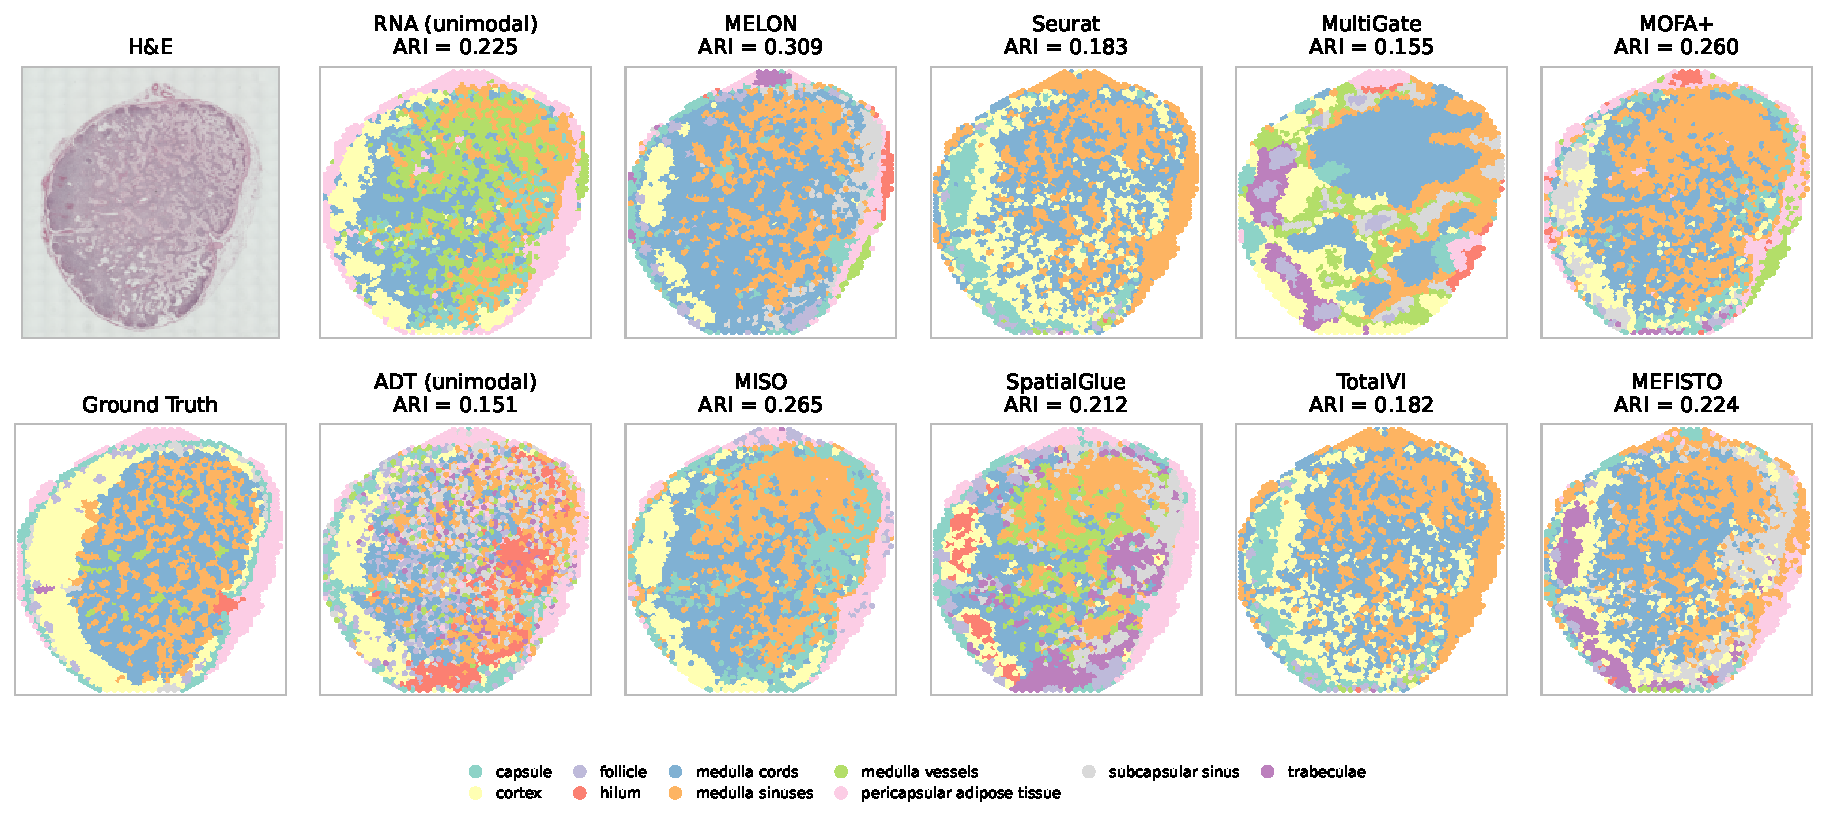
\includegraphics[width=\linewidth]{figures/human_lymph_node_panelC.pdf}
    \caption{H\&E image, ground-truth annotation, and spatial domain assignments from all eight benchmarked methods (ARI labelled per panel; methods ordered consistently across datasets).}
    \label{fig:dataset2_panel_c}
\end{subfigure}

\vspace{0.6ex}
\begin{subfigure}[b]{0.98\textwidth}
    \centering
    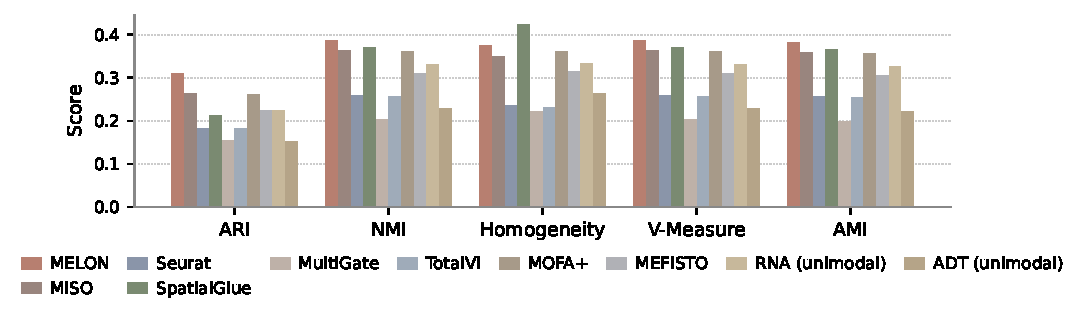
\includegraphics[width=0.90\linewidth]{figures/human_lymph_node_panelD.pdf}
    \caption{Clustering metrics (ARI, NMI, Homogeneity, V-Measure, AMI) across all eight methods at $k=10$.}
    \label{fig:dataset2_panel_d}
\end{subfigure}
\caption{Human lymph node results. (a) H\&E tissue image, ground-truth annotation, and spatial domain assignments from MELON and seven multimodal baselines (per-panel ARI). (b) Five clustering metrics across all eight methods. Benchmark-over-$k$ curves are provided in Appendix~\ref{fig:app-dataset2-metrics}.}
\label{fig:dataset2_results}
\end{figure}

\begin{figure}[!ht]
\centering
\begin{subfigure}[b]{0.98\textwidth}
    \centering
    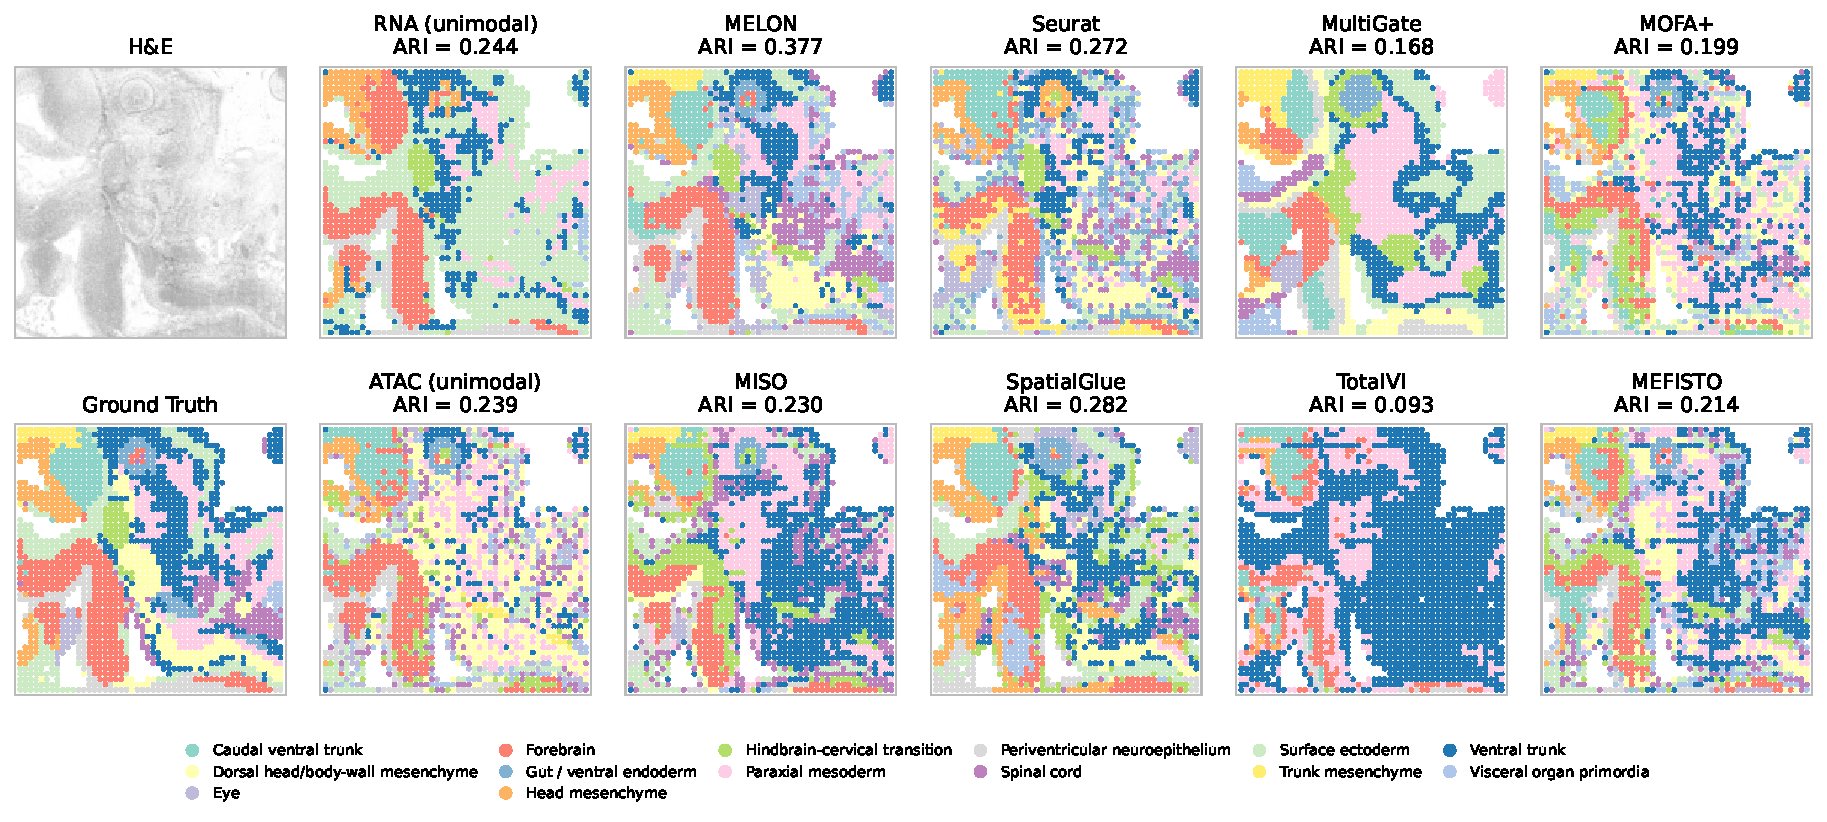
\includegraphics[width=\linewidth]{figures/mouse_embryo_panelC.pdf}
    \caption{H\&E image, ground-truth annotation, and spatial domain assignments from all eight benchmarked methods (ARI labelled per panel; methods ordered consistently across datasets).}
    \label{fig:dataset3_panel_c}
\end{subfigure}

\vspace{0.6ex}
\begin{subfigure}[b]{0.98\textwidth}
    \centering
    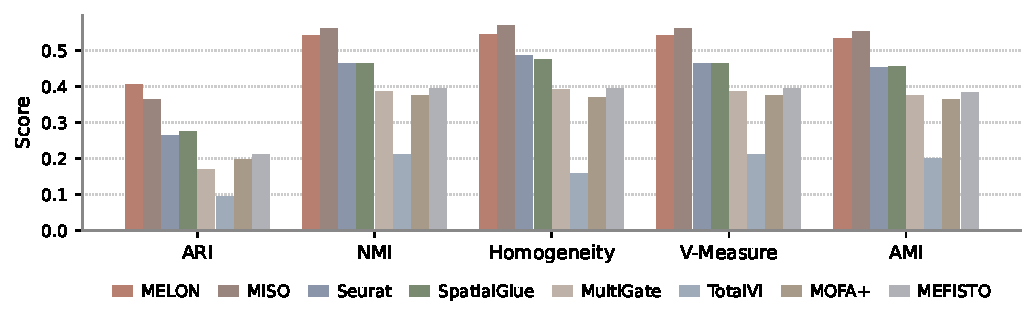
\includegraphics[width=0.90\linewidth]{figures/mouse_embryo_panelD.pdf}
    \caption{Clustering metrics (ARI, NMI, Homogeneity, V-Measure, AMI) across all eight methods at $k=14$.}
    \label{fig:dataset3_panel_d}
\end{subfigure}
\caption{Mouse E13 embryo results. (a) H\&E tissue image, ground-truth annotation, and spatial domain assignments from MELON and seven multimodal baselines (per-panel ARI). (b) Five clustering metrics across all eight methods. Benchmark-over-$k$ curves are provided in Appendix~\ref{fig:app-dataset3-metrics}.}
\label{fig:dataset3_results}
\end{figure}

\subsection{Benchmarking Metrics Across Methods}

\begin{figure}[!ht]
\centering
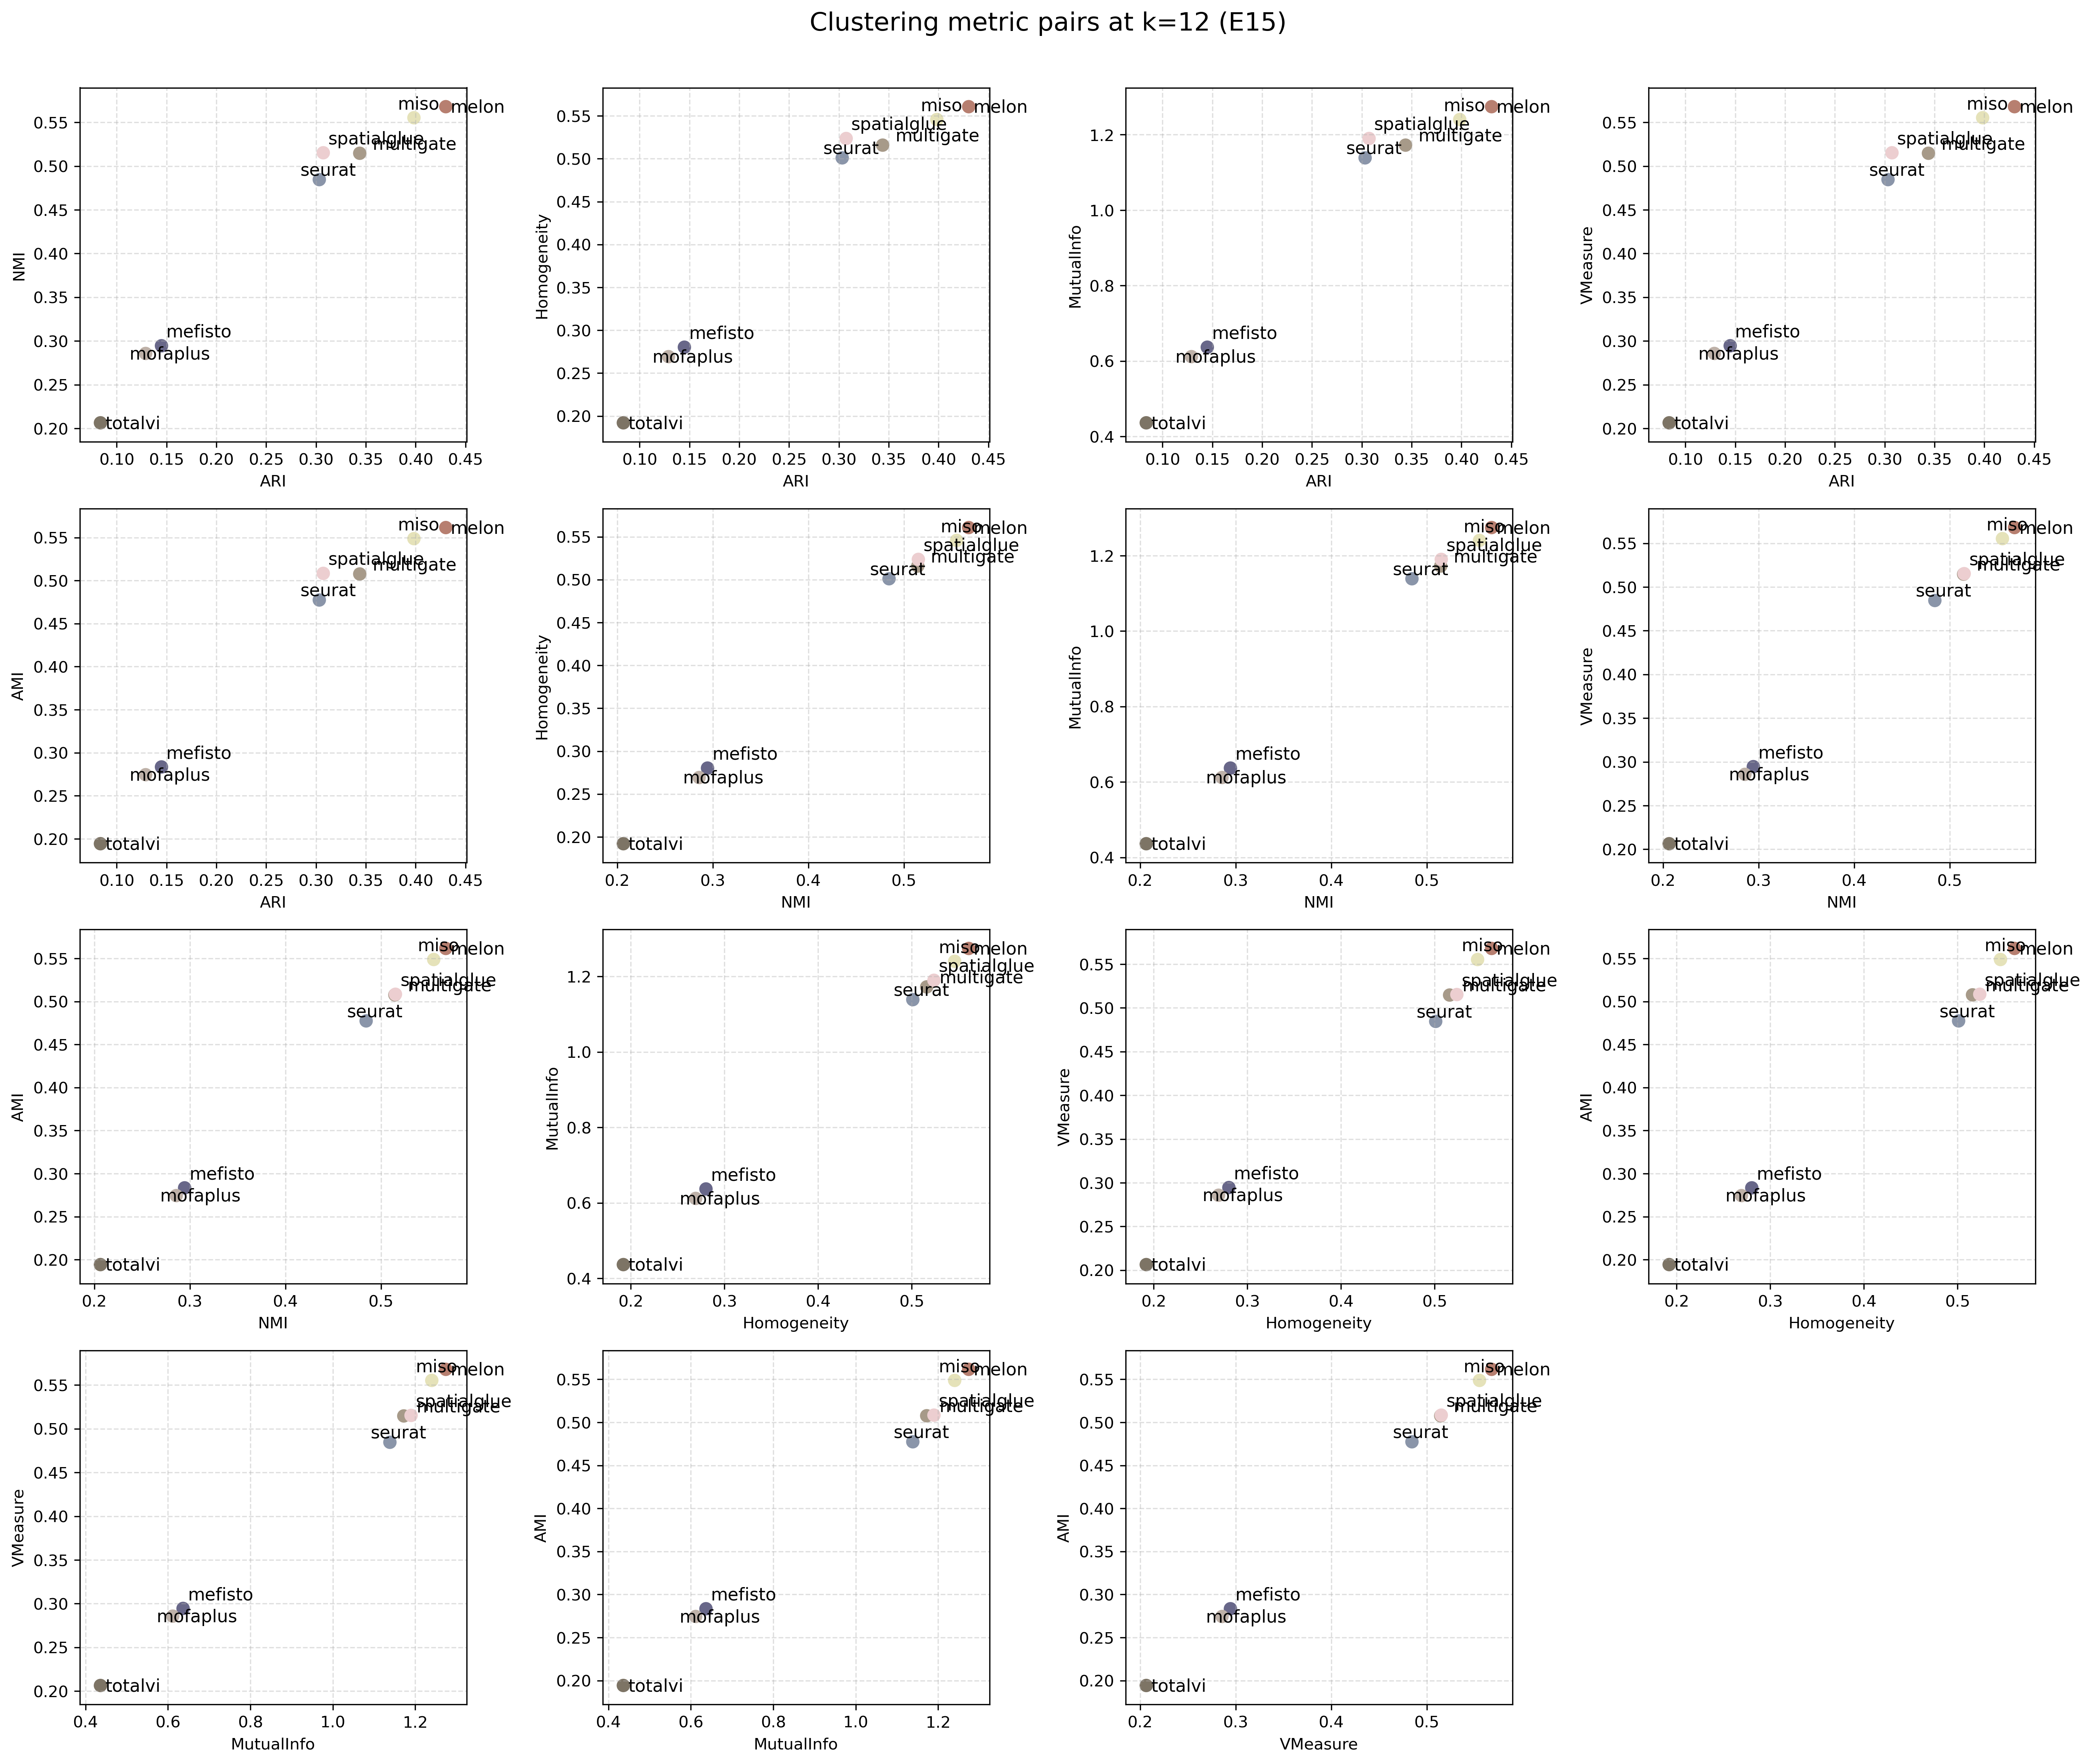
\includegraphics[width=0.72\textwidth]{figures/benchmarking_metrics_k12_e15.png}
\caption{Appendix benchmark-over-$k$ metrics for the Mouse E15.5 brain dataset.}
\label{fig:app-dataset1-metrics}
\end{figure}

\begin{figure}[!ht]
\centering
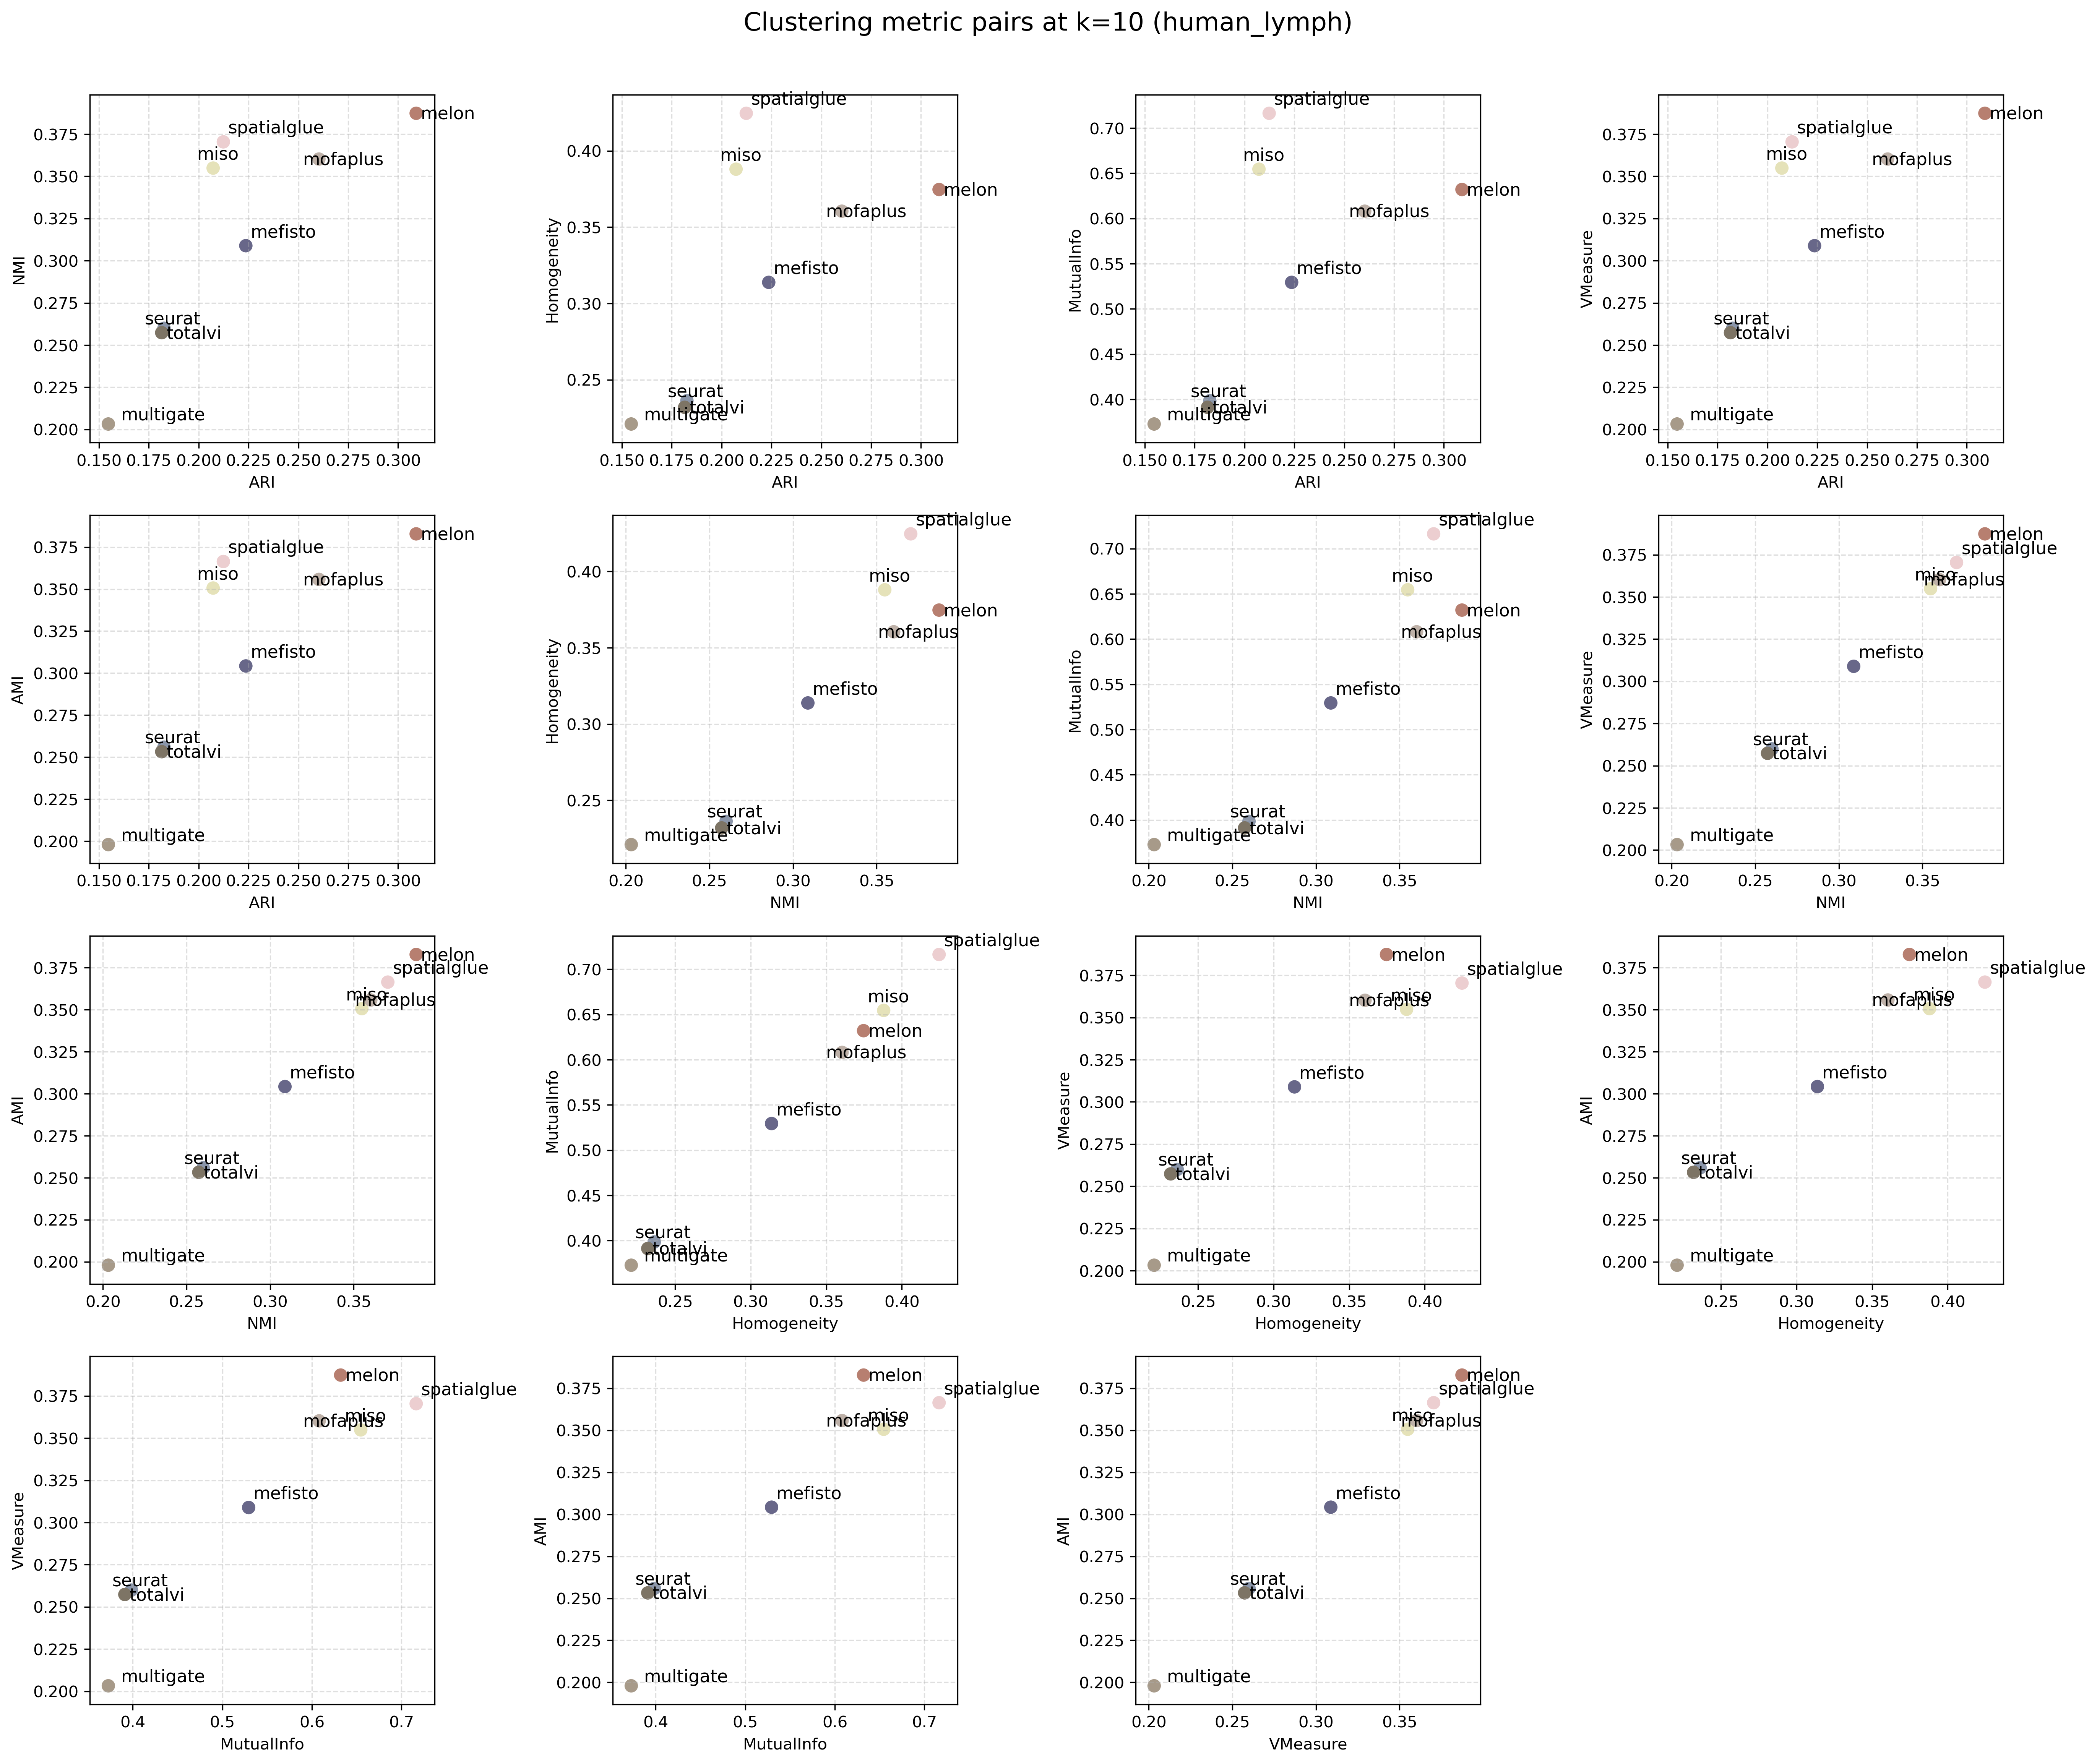
\includegraphics[width=0.72\textwidth]{figures/benchmarking_metrics_k10_human_lymph.png}
\caption{Appendix benchmark-over-$k$ metrics for the Human lymph node dataset.}
\label{fig:app-dataset2-metrics}
\end{figure}

\begin{figure}[!ht]
\centering
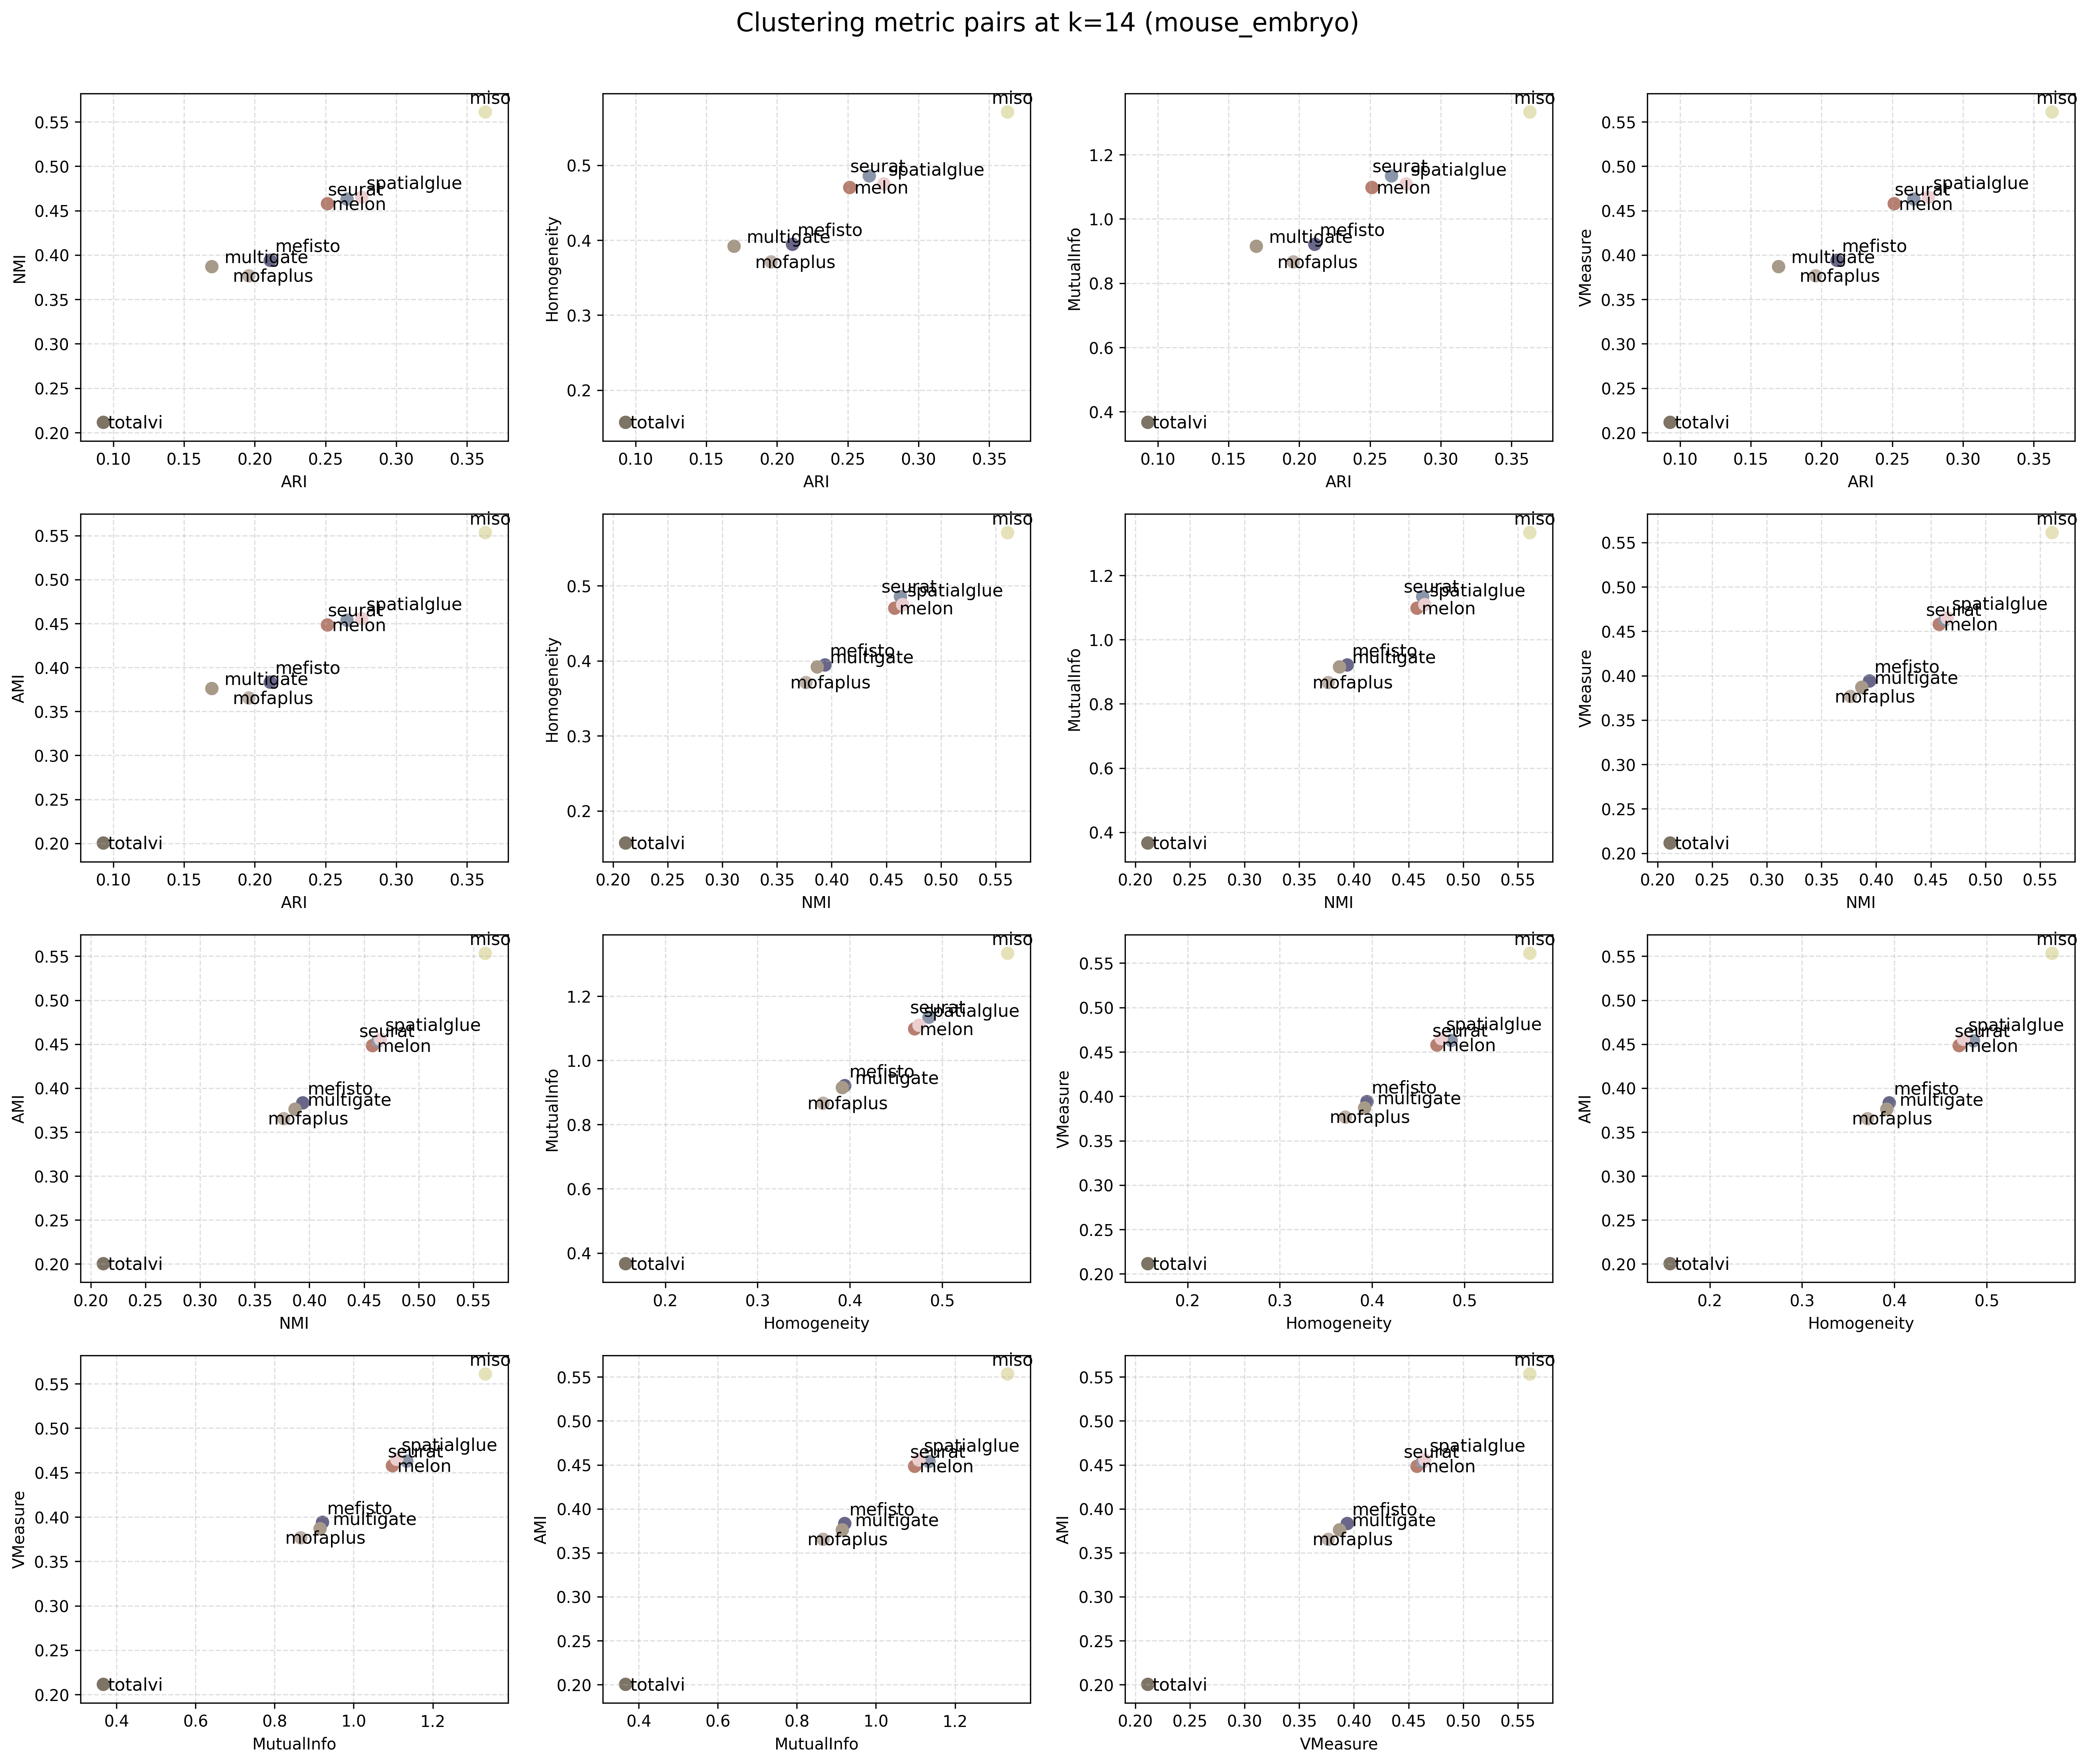
\includegraphics[width=0.72\textwidth]{figures/benchmarking_metrics_k14_mouse_embryo.png}
\caption{Appendix benchmark-over-$k$ metrics for the Mouse E13 embryo dataset.}
\label{fig:app-dataset3-metrics}
\end{figure}

\subsection{Sensitivity Analysis}
We evaluate the sensitivity of MELON to its main hyperparameters, including the (1) number of spatial neighbors $k$, (2) latent dimension, (3) number of fusion layers, and (4) contrastive temperature. The results show that MELON is stable over a broad range of settings, with only moderate degradation under substantial perturbations.

\paragraph{Number of spatial neighbors.}
We sweep the spatial graph size $k \in \{1, 2, 4, 8, 16, 32\}$ on the simulation benchmark and probe the frozen embedding for the four latent factors (shared $Y$, modality-specific $R$ and $U$, and common signal $C$). As shown in Figure~\ref{fig:app-neighbor-k-sensitivity}, the modality-specific and common factors ($R$, $U$, $C$) are recovered essentially perfectly across the entire range, while balanced accuracy on the shared label $Y$ stays within a narrow $0.78$--$0.84$ band, with overlapping error bars across all $k$. Performance is therefore robust to reasonable changes in neighborhood size, indicating that MELON does not rely on carefully tuned local graph construction. Very small ($k{=}1$) and very large ($k{=}32$) neighborhoods behave comparably to the default $k{=}8$, suggesting that the spatial bias injected by NeighborhoodGAT degrades gracefully rather than collapsing when the graph is mis-specified.

\begin{figure}[!ht]
\centering
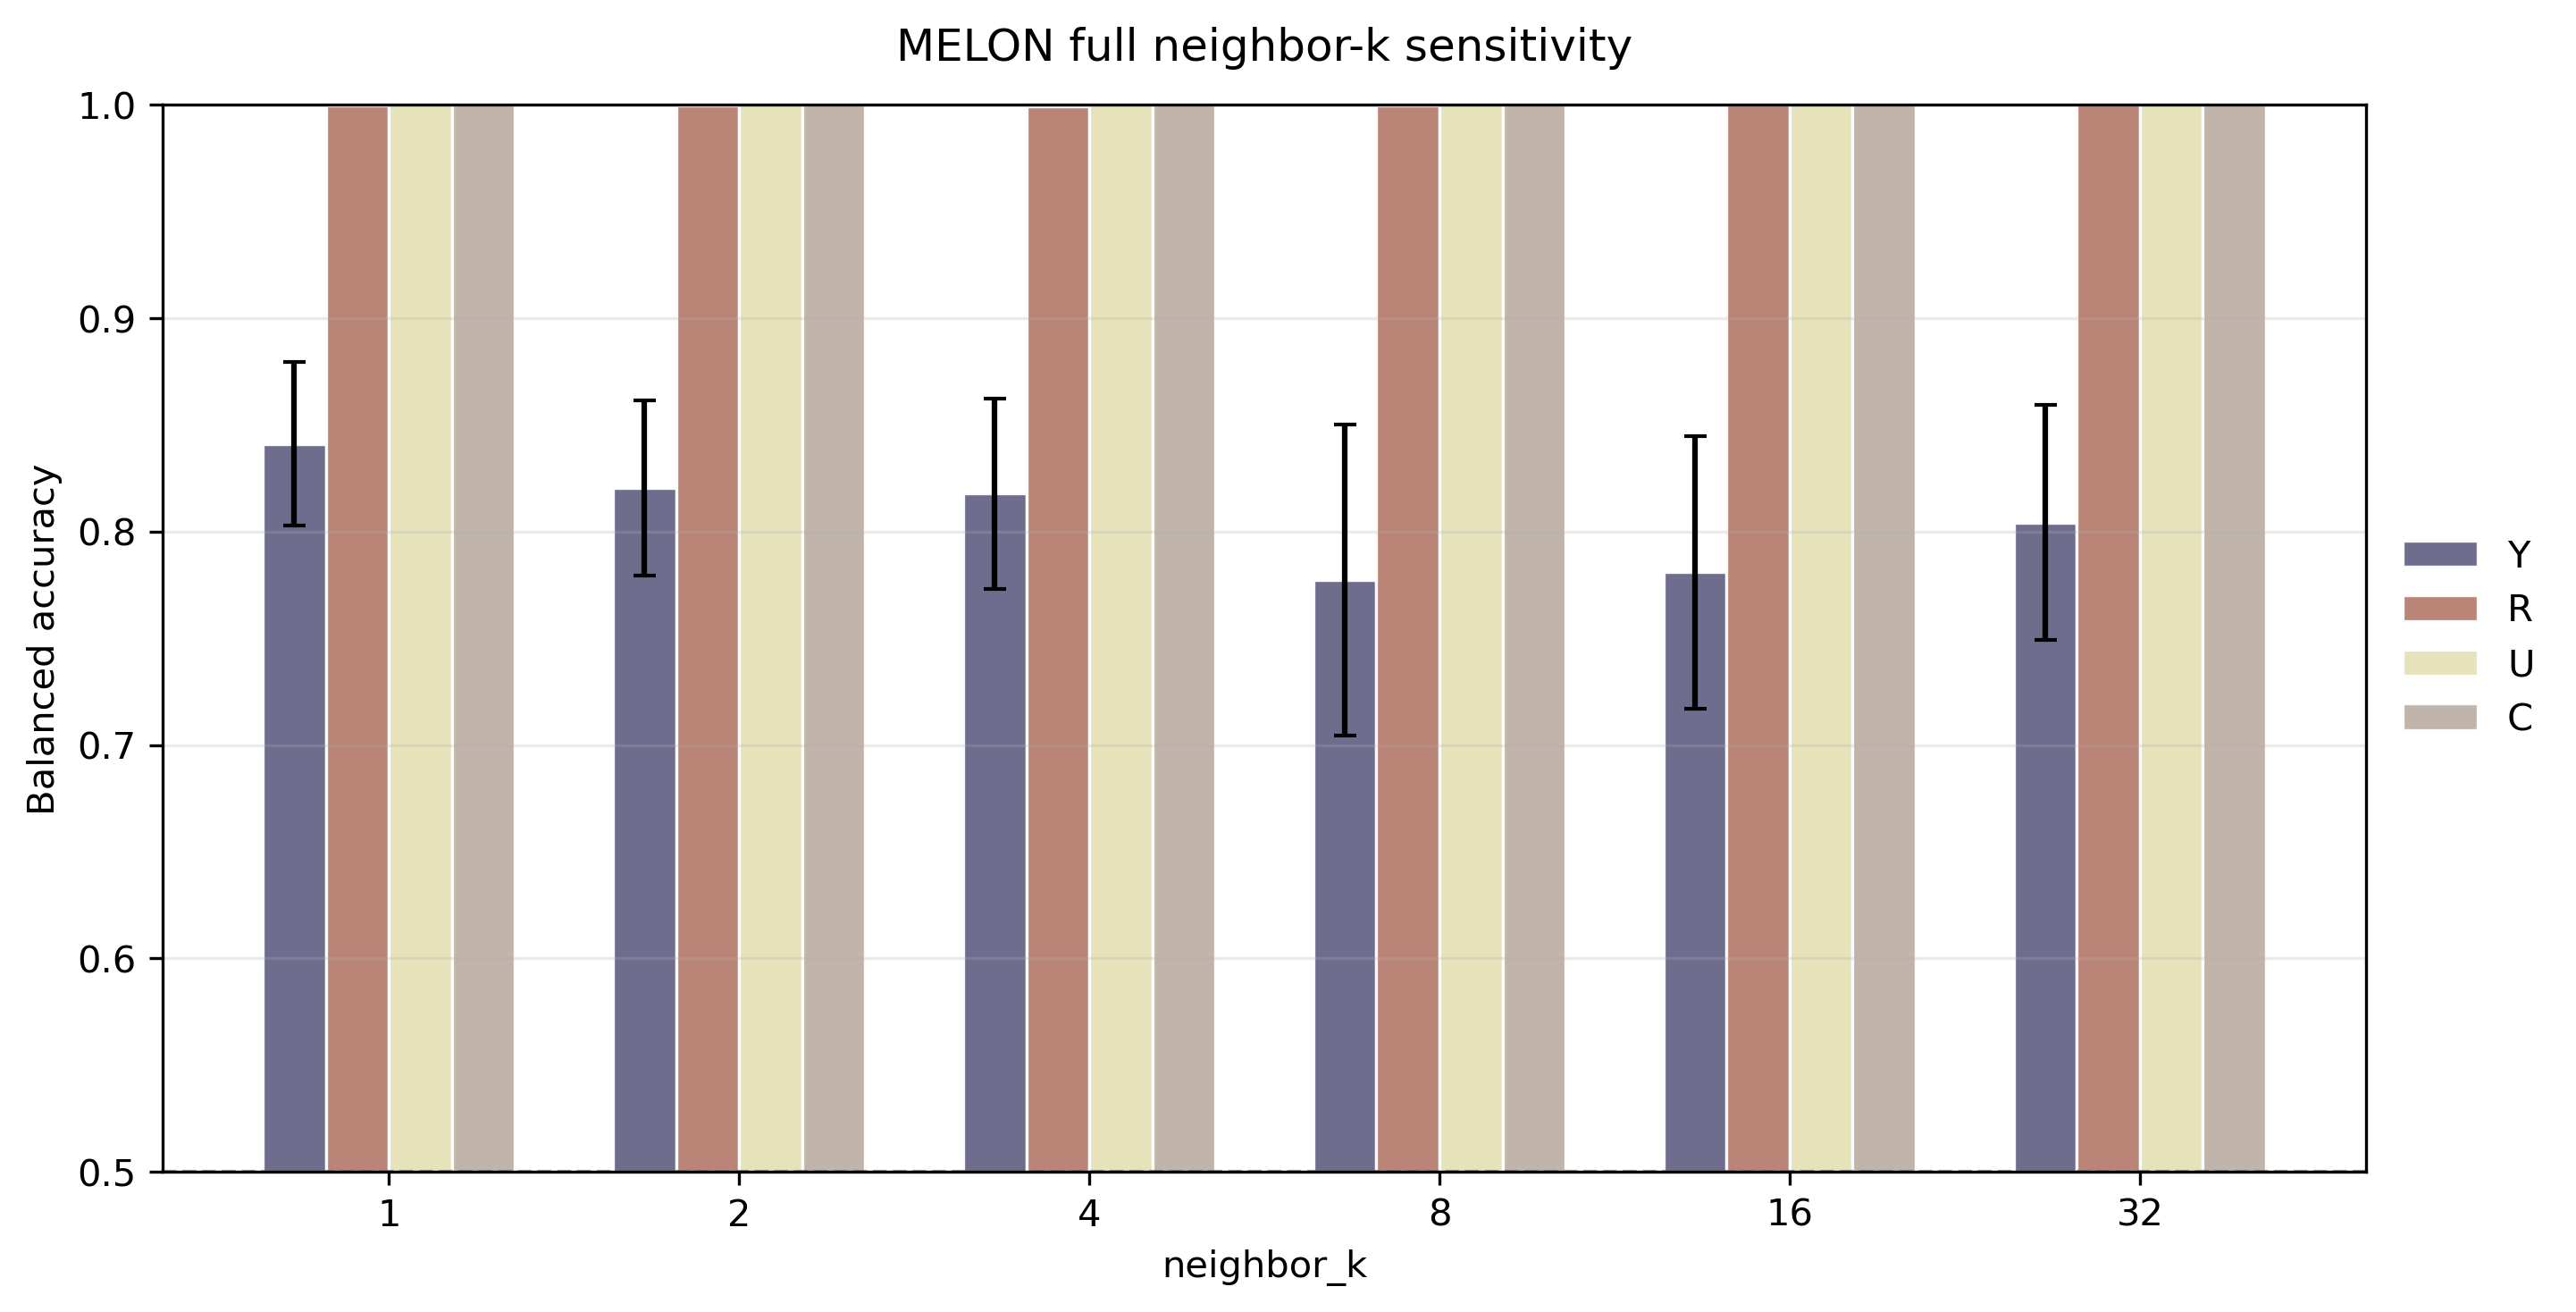
\includegraphics[width=0.9\textwidth]{figures/fig_neighbor_k_sensitivity.png}
\caption{Sensitivity of MELON to the number of spatial neighbors $k$ on the simulation benchmark. Bars show balanced accuracy (mean $\pm$ std over seeds) for probing the shared label $Y$, modality-specific factors $R$ and $U$, and the common signal $C$, at $k \in \{1, 2, 4, 8, 16, 32\}$. Recovery of $R$, $U$, and $C$ is saturated across all $k$, and $Y$ accuracy varies by less than $0.07$ across a $32\times$ range of neighborhood sizes.}
\label{fig:app-neighbor-k-sensitivity}
\end{figure}

\paragraph{Other hyperparameters.}
Varying the latent dimension or transformer depth produces relatively small fluctuations compared with the gap to baselines, indicating that MELON’s gains are architectural rather than incidental. We also test sensitivity to the relative weighting of the multimodal and unimodal contrastive terms and find that the model is most stable when both are retained, which is consistent with the goal of preserving both shared and modality-specific signal. These results suggest that MELON is not only accurate but also practically robust across datasets with different modality characteristics and spatial resolutions.

\subsection{Interpretability}\label{app:interpretability}
We probe MELON's frozen embedding with a joint pair-decoder and ask whether the resulting factors recover biologically meaningful, spatially organized RNA--ATAC (or RNA--protein) programs.

\paragraph{Decoder formulation.}
Let $\mathbf{z}_i \in \mathbb{R}^{d}$ denote the frozen MELON fused embedding of spot $i$, and let $\mathbf{x}^{R}_i \in \mathbb{R}^{G}$ and $\mathbf{x}^{A}_i \in \{0,1\}^{P}$ be its observed RNA expression and binarised ATAC (or protein) profile, where $G$ and $P$ are the number of genes and peaks respectively. We map each embedding through a small MLP $\phi$ with a low-rank bottleneck of width $K$ (we use $K{=}24$ for the two RNA--ATAC datasets and $K{=}16$ for the lymph node):
\begin{equation}\label{eq:decoder-bottleneck}
    \mathbf{u}_i \;=\; \mathrm{softplus}\!\bigl(\phi(\mathbf{z}_i)\bigr) \;\in\; \mathbb{R}_{\geq 0}^{K},
\end{equation}
so that $u_{i,k}$ is the non-negative usage of factor $k$ at spot $i$. Two linear heads decode this bottleneck back into the two modalities,
\begin{equation}\label{eq:decoder-heads}
    \widehat{\mathbf{x}}^{R}_i \;=\; \mathbf{W}^{R}\,\mathbf{u}_i \;+\; \mathbf{b}^{R},
    \qquad
    \widehat{\mathbf{x}}^{A}_i \;=\; \sigma\!\bigl(\mathbf{W}^{A}\,\mathbf{u}_i \;+\; \mathbf{b}^{A}\bigr),
\end{equation}
with $\mathbf{W}^{R} \in \mathbb{R}^{G \times K}$, $\mathbf{W}^{A} \in \mathbb{R}^{P \times K}$ and $\sigma$ the elementwise sigmoid. The two-headed reconstruction loss couples both modalities through the same factor activations,
\begin{equation}\label{eq:decoder-loss}
    \mathcal{L}_{\text{dec}}
    \;=\; \frac{1}{N}\sum_{i=1}^{N}\Bigl[
        \bigl\|\mathbf{x}^{R}_i - \widehat{\mathbf{x}}^{R}_i\bigr\|_{2}^{2}
        \;+\; \lambda\,
        \mathrm{BCE}\!\bigl(\mathbf{x}^{A}_i,\,\widehat{\mathbf{x}}^{A}_i\bigr)
    \Bigr],
\end{equation}
where $\mathrm{BCE}(\cdot,\cdot)$ is the elementwise binary cross-entropy averaged over peaks/proteins and $\lambda$ balances the two heads (we use $\lambda{=}1$). Only the decoder parameters $\{\phi, \mathbf{W}^{R}, \mathbf{b}^{R}, \mathbf{W}^{A}, \mathbf{b}^{A}\}$ are trained; MELON is frozen. We optimise with Adam for 20 epochs on a 90/10 train--validation split.

\paragraph{Per-factor feature ranking.}
After training, factor $k$ is summarised by three quantities: (i) its \emph{spatial usage} $\{u_{i,k}\}_{i=1}^{N}$, plotted on tissue coordinates; (ii) its \emph{top gene} and \emph{top peak/protein}, defined as the columns of $\mathbf{W}^{R}$ and $\mathbf{W}^{A}$ with the largest loading on factor $k$,
\begin{equation}\label{eq:top-feature}
    g^{\star}_k \;=\; \arg\max_{g \in [G]} W^{R}_{g,k},
    \qquad
    p^{\star}_k \;=\; \arg\max_{p \in [P]} W^{A}_{p,k};
\end{equation}
and (iii) its \emph{top gene--peak pair score}, defined as the product of the two loadings,
\begin{equation}\label{eq:pair-score}
    s_{g,p,k} \;=\; W^{R}_{g,k}\,\cdot\,W^{A}_{p,k},
    \qquad
    (g^{\dagger}_k, p^{\dagger}_k) \;=\; \arg\max_{(g,p)} s_{g,p,k}.
\end{equation}
This product score promotes pairs in which the gene and the peak load on the \emph{same} factor with high magnitude, so that a high score identifies cross-modal feature pairs jointly explained by a shared latent program. We rank all $G\!\times\!P$ pairs per factor by~\eqref{eq:pair-score} and report the top entries in the supplementary CSVs.

\paragraph{Decoder factor program maps.}
For each dataset we show four high-variance factors with their top gene and top peak (or protein) label as Figures~\ref{fig:e15-decoder-factors}, \ref{fig:hln-decoder-factors}, and \ref{fig:embryo-decoder-factors}. The mouse E13 embryo factors (0, 14, 8, 19) have biologically named top pairs including \emph{Cdh19--Pmpcb} (factor~0; \emph{Cdh19} is a cadherin involved in neural crest development) and \emph{Mak--Pou3f1} (factor~14; \emph{Pou3f1} marks early neural progenitors). The mouse E15.5 brain factors carry chromosomal-coordinate ATAC peaks that we abbreviate to \texttt{chrN:Mb} for display. The human lymph node decoder collapses every factor's top protein loading to the dominant cytokeratin marker KRT5 (which has prevalence $\approx 0.76$ across the section), but the per-spot factor usage still clearly separates follicular and cortical-medullary territories. The remaining factors and full feature loadings are reported in the supplementary CSVs (\texttt{factor\_top\_genes.csv}, \texttt{factor\_top\_peaks.csv}, \texttt{factor\_top\_pairs.csv}) for each decoder.

\begin{figure}[!ht]
\centering
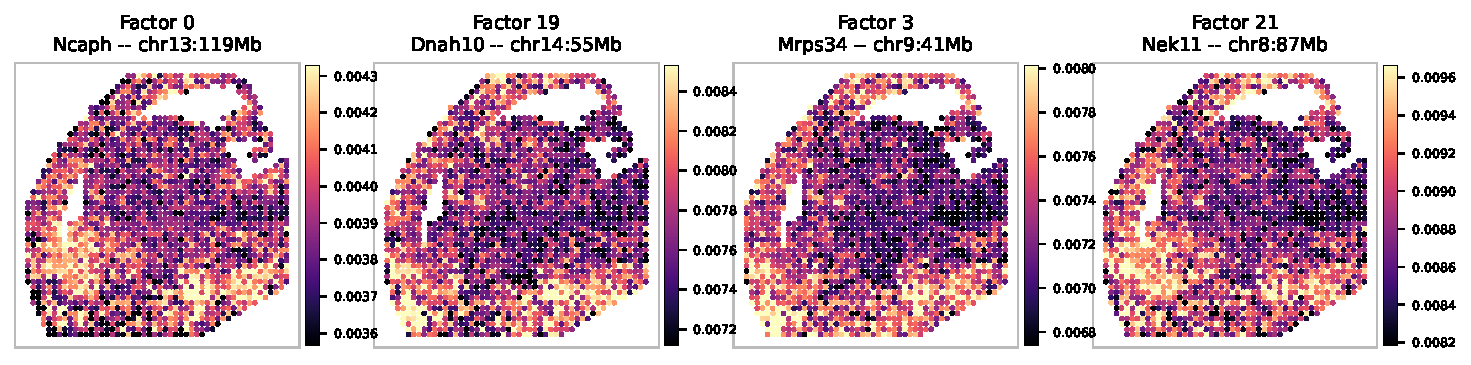
\includegraphics[width=0.96\textwidth]{figures/mouse_e15_brain_decoder_factors.pdf}
\caption{Mouse E15.5 brain. Spatial usage of four MELON decoder factors with the top gene and top ATAC peak (chromosomal coordinate, abbreviated to \texttt{chrN:Mb}) shown above each panel. Color is per-factor robust-clipped (5--95\%) usage from the 24-factor pair decoder.}
\label{fig:e15-decoder-factors}
\end{figure}

\begin{figure}[!ht]
\centering
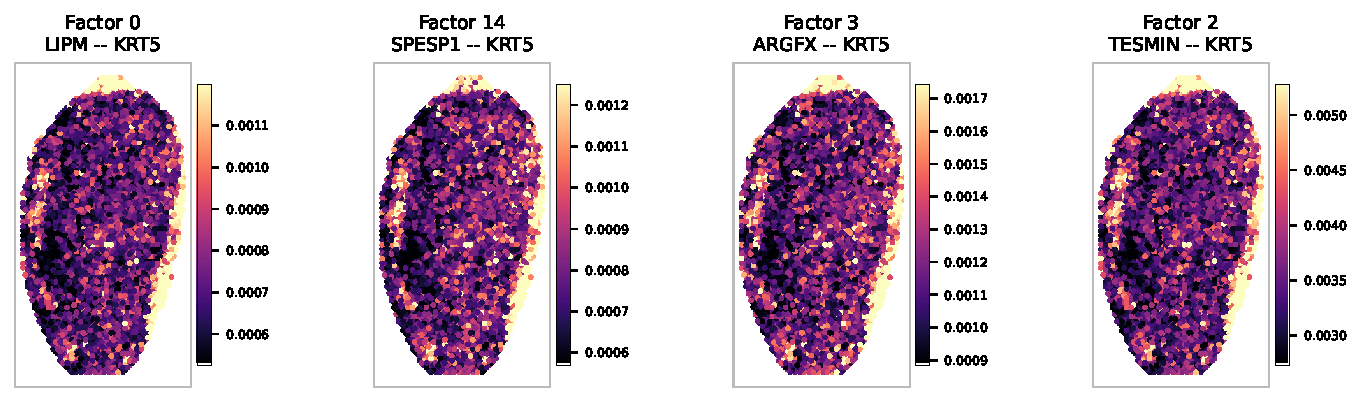
\includegraphics[width=0.96\textwidth]{figures/human_lymph_decoder_factors.pdf}
\caption{Human lymph node. Spatial usage of four MELON decoder factors, with the top gene for each factor shown. The dominant protein loading collapses to KRT5 across all factors, but the per-spot factor usage still cleanly separates anatomical compartments.}
\label{fig:hln-decoder-factors}
\end{figure}

\begin{figure}[!ht]
\centering
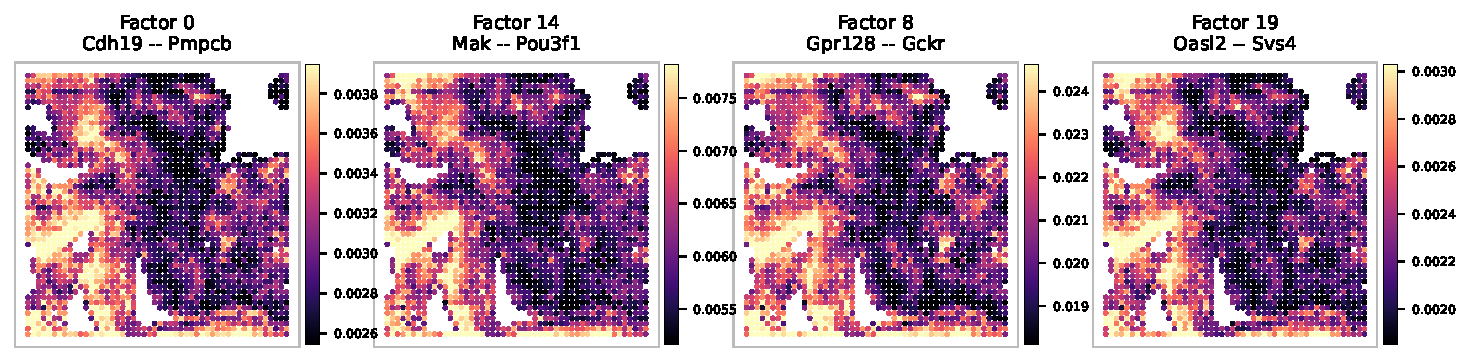
\includegraphics[width=0.96\textwidth]{figures/mouse_embryo_decoder_factors.pdf}
\caption{Mouse E13 embryo. Spatial usage of four MELON decoder factors with the top gene--peak pair shown above each panel. Each factor concentrates in a distinct anatomical region, demonstrating that the frozen embedding can be decoded into spatially coherent joint RNA/ATAC programs.}
\label{fig:embryo-decoder-factors}
\end{figure}

\paragraph{High-support gene--peak pair maps.}
As an additional perspective we select six gene--peak pairs per dataset from the global top-pair list whose joint score exceeds a coverage threshold, and visualize each pair's RNA expression, ATAC accessibility (or protein abundance for the lymph node), and decoder pair-activity on the tissue coordinates side by side (Figures~\ref{fig:e15-decoder-pairs}, \ref{fig:hln-decoder-pairs}, and \ref{fig:embryo-decoder-pairs}). Several of these pairs show concentrated activity patterns that are not explained by either modality in isolation -- the per-spot pair activity has a sharper boundary than the marginal RNA or ATAC channel alone -- consistent with the claim that MELON's embedding preserves cross-modal correspondence rather than collapsing to a shared consensus. We caution that the global top-pair list is dominated by ubiquitous peaks for the embryo and lymph node decoders (peak/protein prevalence approaching $1.0$ for several entries), so the factor-based analysis in main text is the more robust summary; the per-pair maps are included for completeness.

\begin{figure}[!ht]
\centering
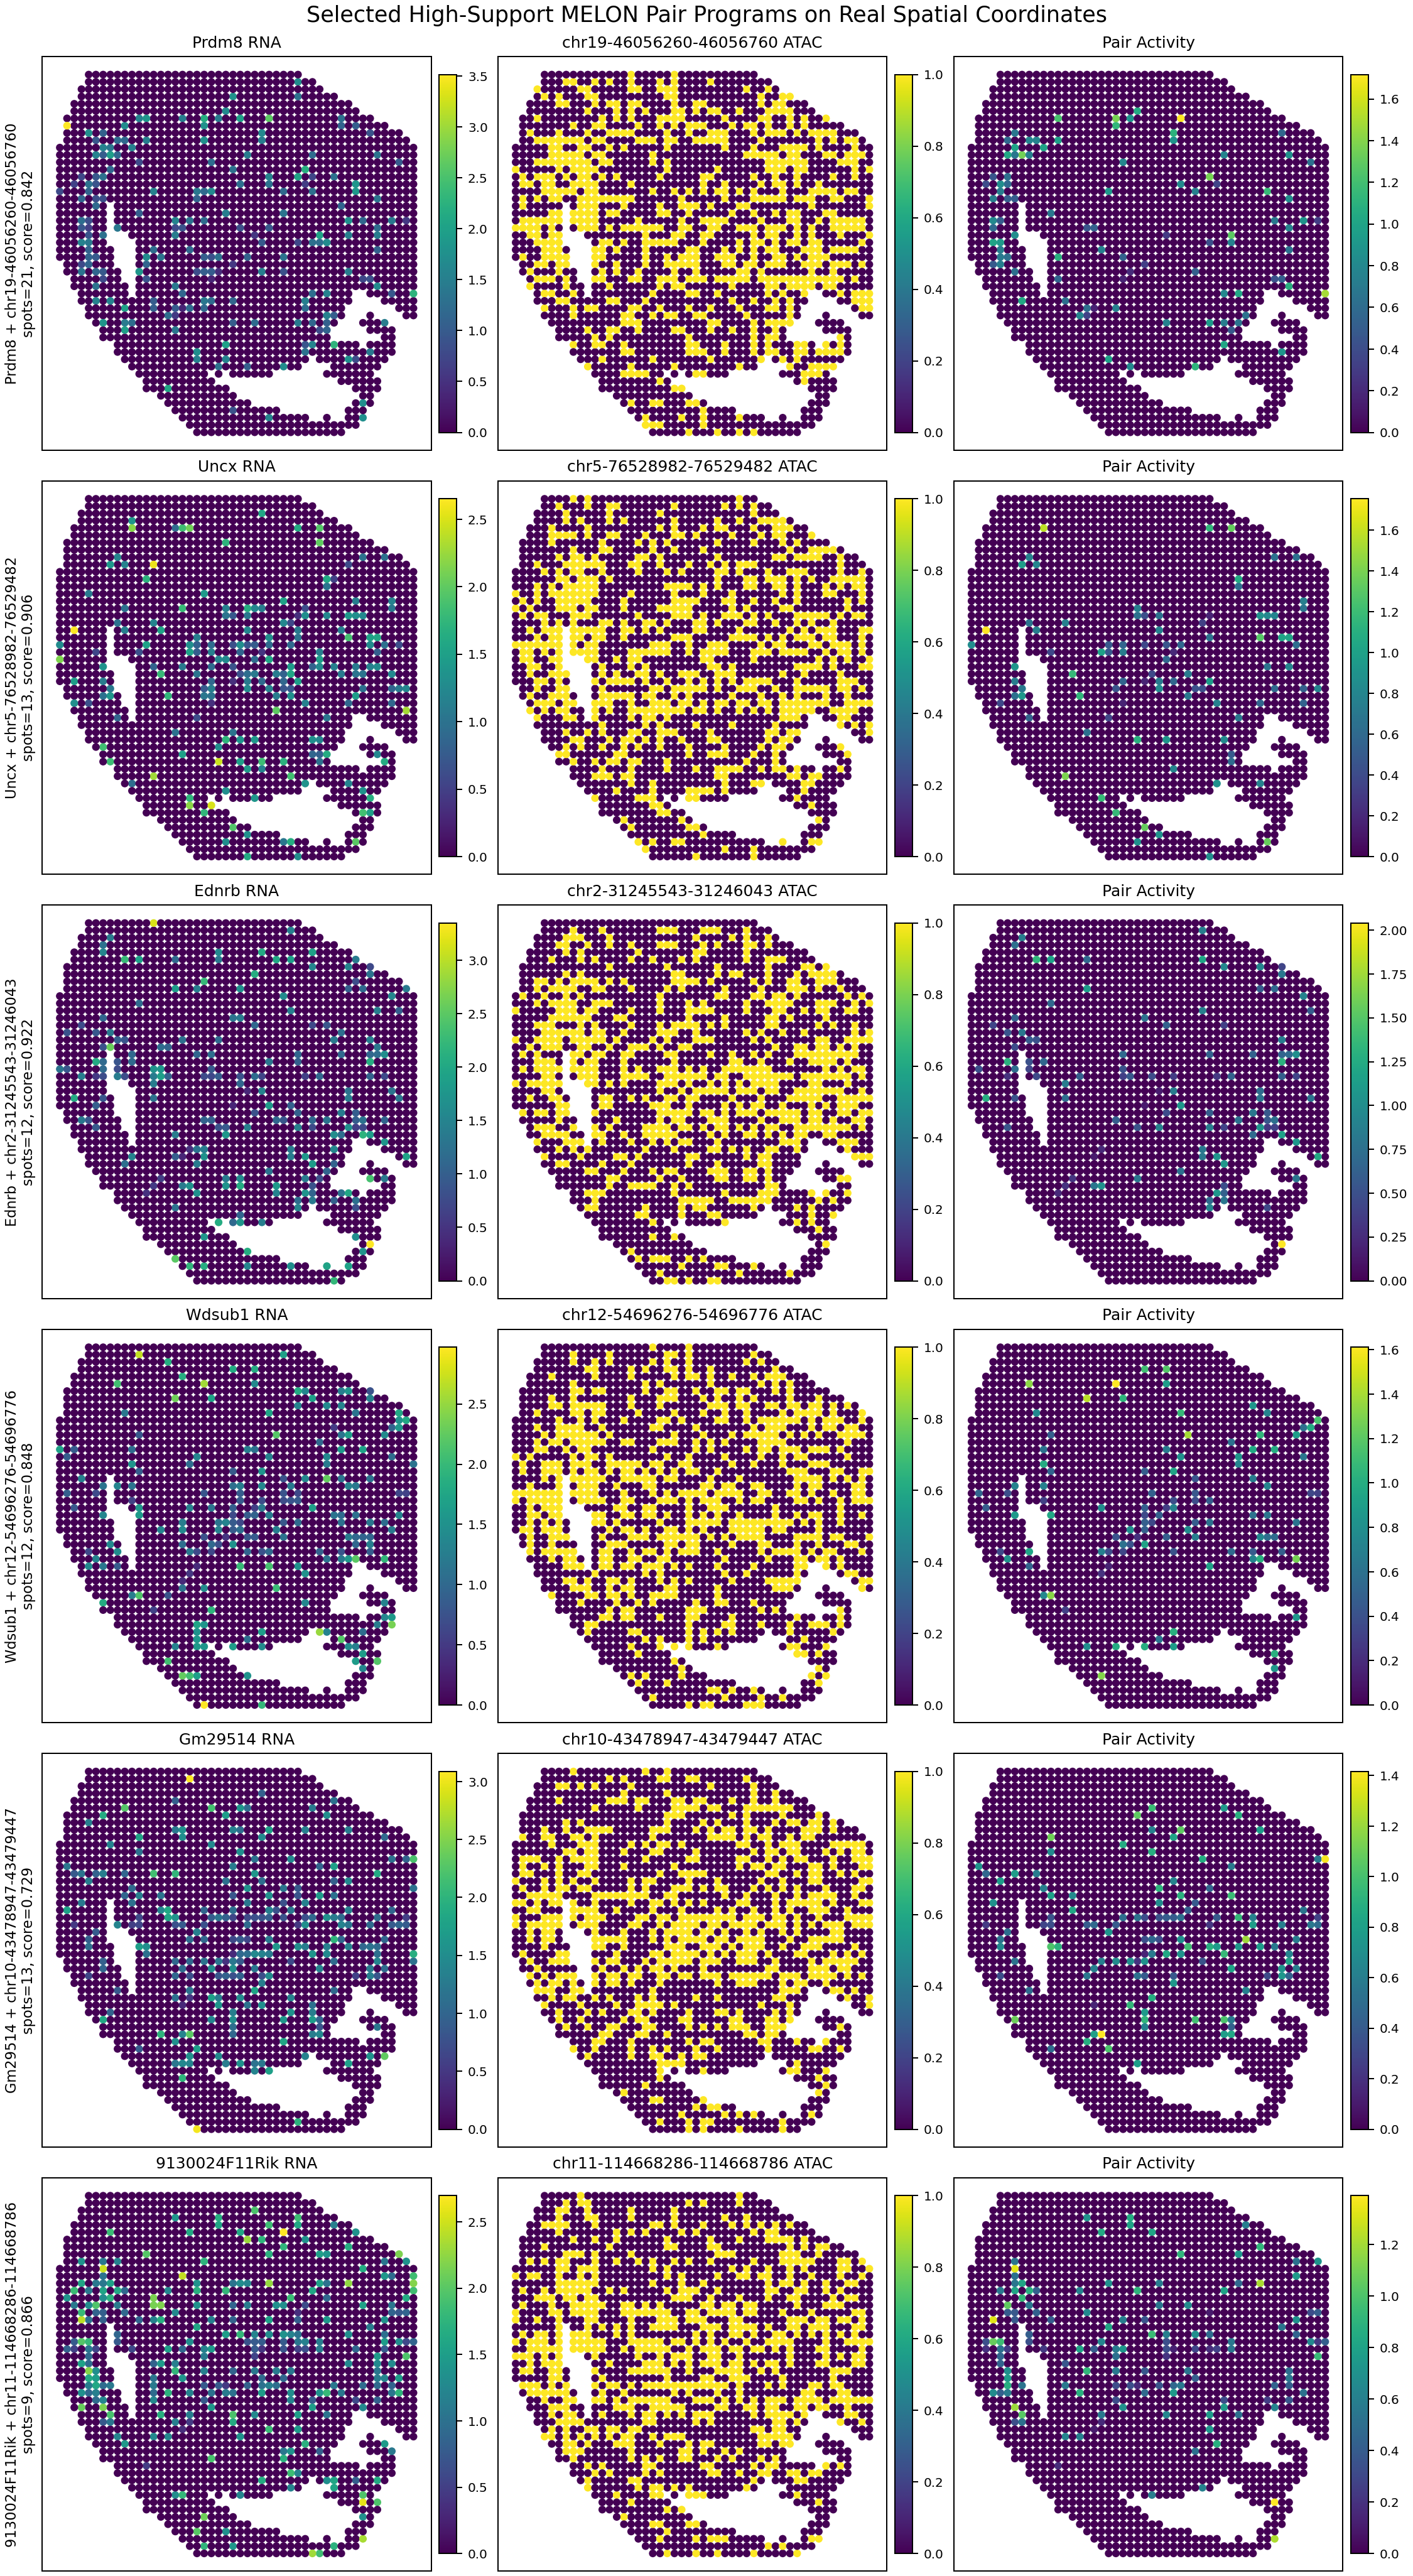
\includegraphics[width=0.75\textwidth]{figures/mouse_e15_brain_decoder_pair_maps.png}
\caption{Mouse E15.5 brain. Spatial maps for six high-support gene--peak pairs from the decoder. Each row is one pair; columns show (left) RNA expression of the gene, (centre) ATAC accessibility of the peak, and (right) the decoder's joint pair activity. Top pairs include \emph{Prdm8}, \emph{Uncx}, and \emph{Ednrb}, all known developmental transcription factors / receptors.}
\label{fig:e15-decoder-pairs}
\end{figure}

\begin{figure}[!ht]
\centering
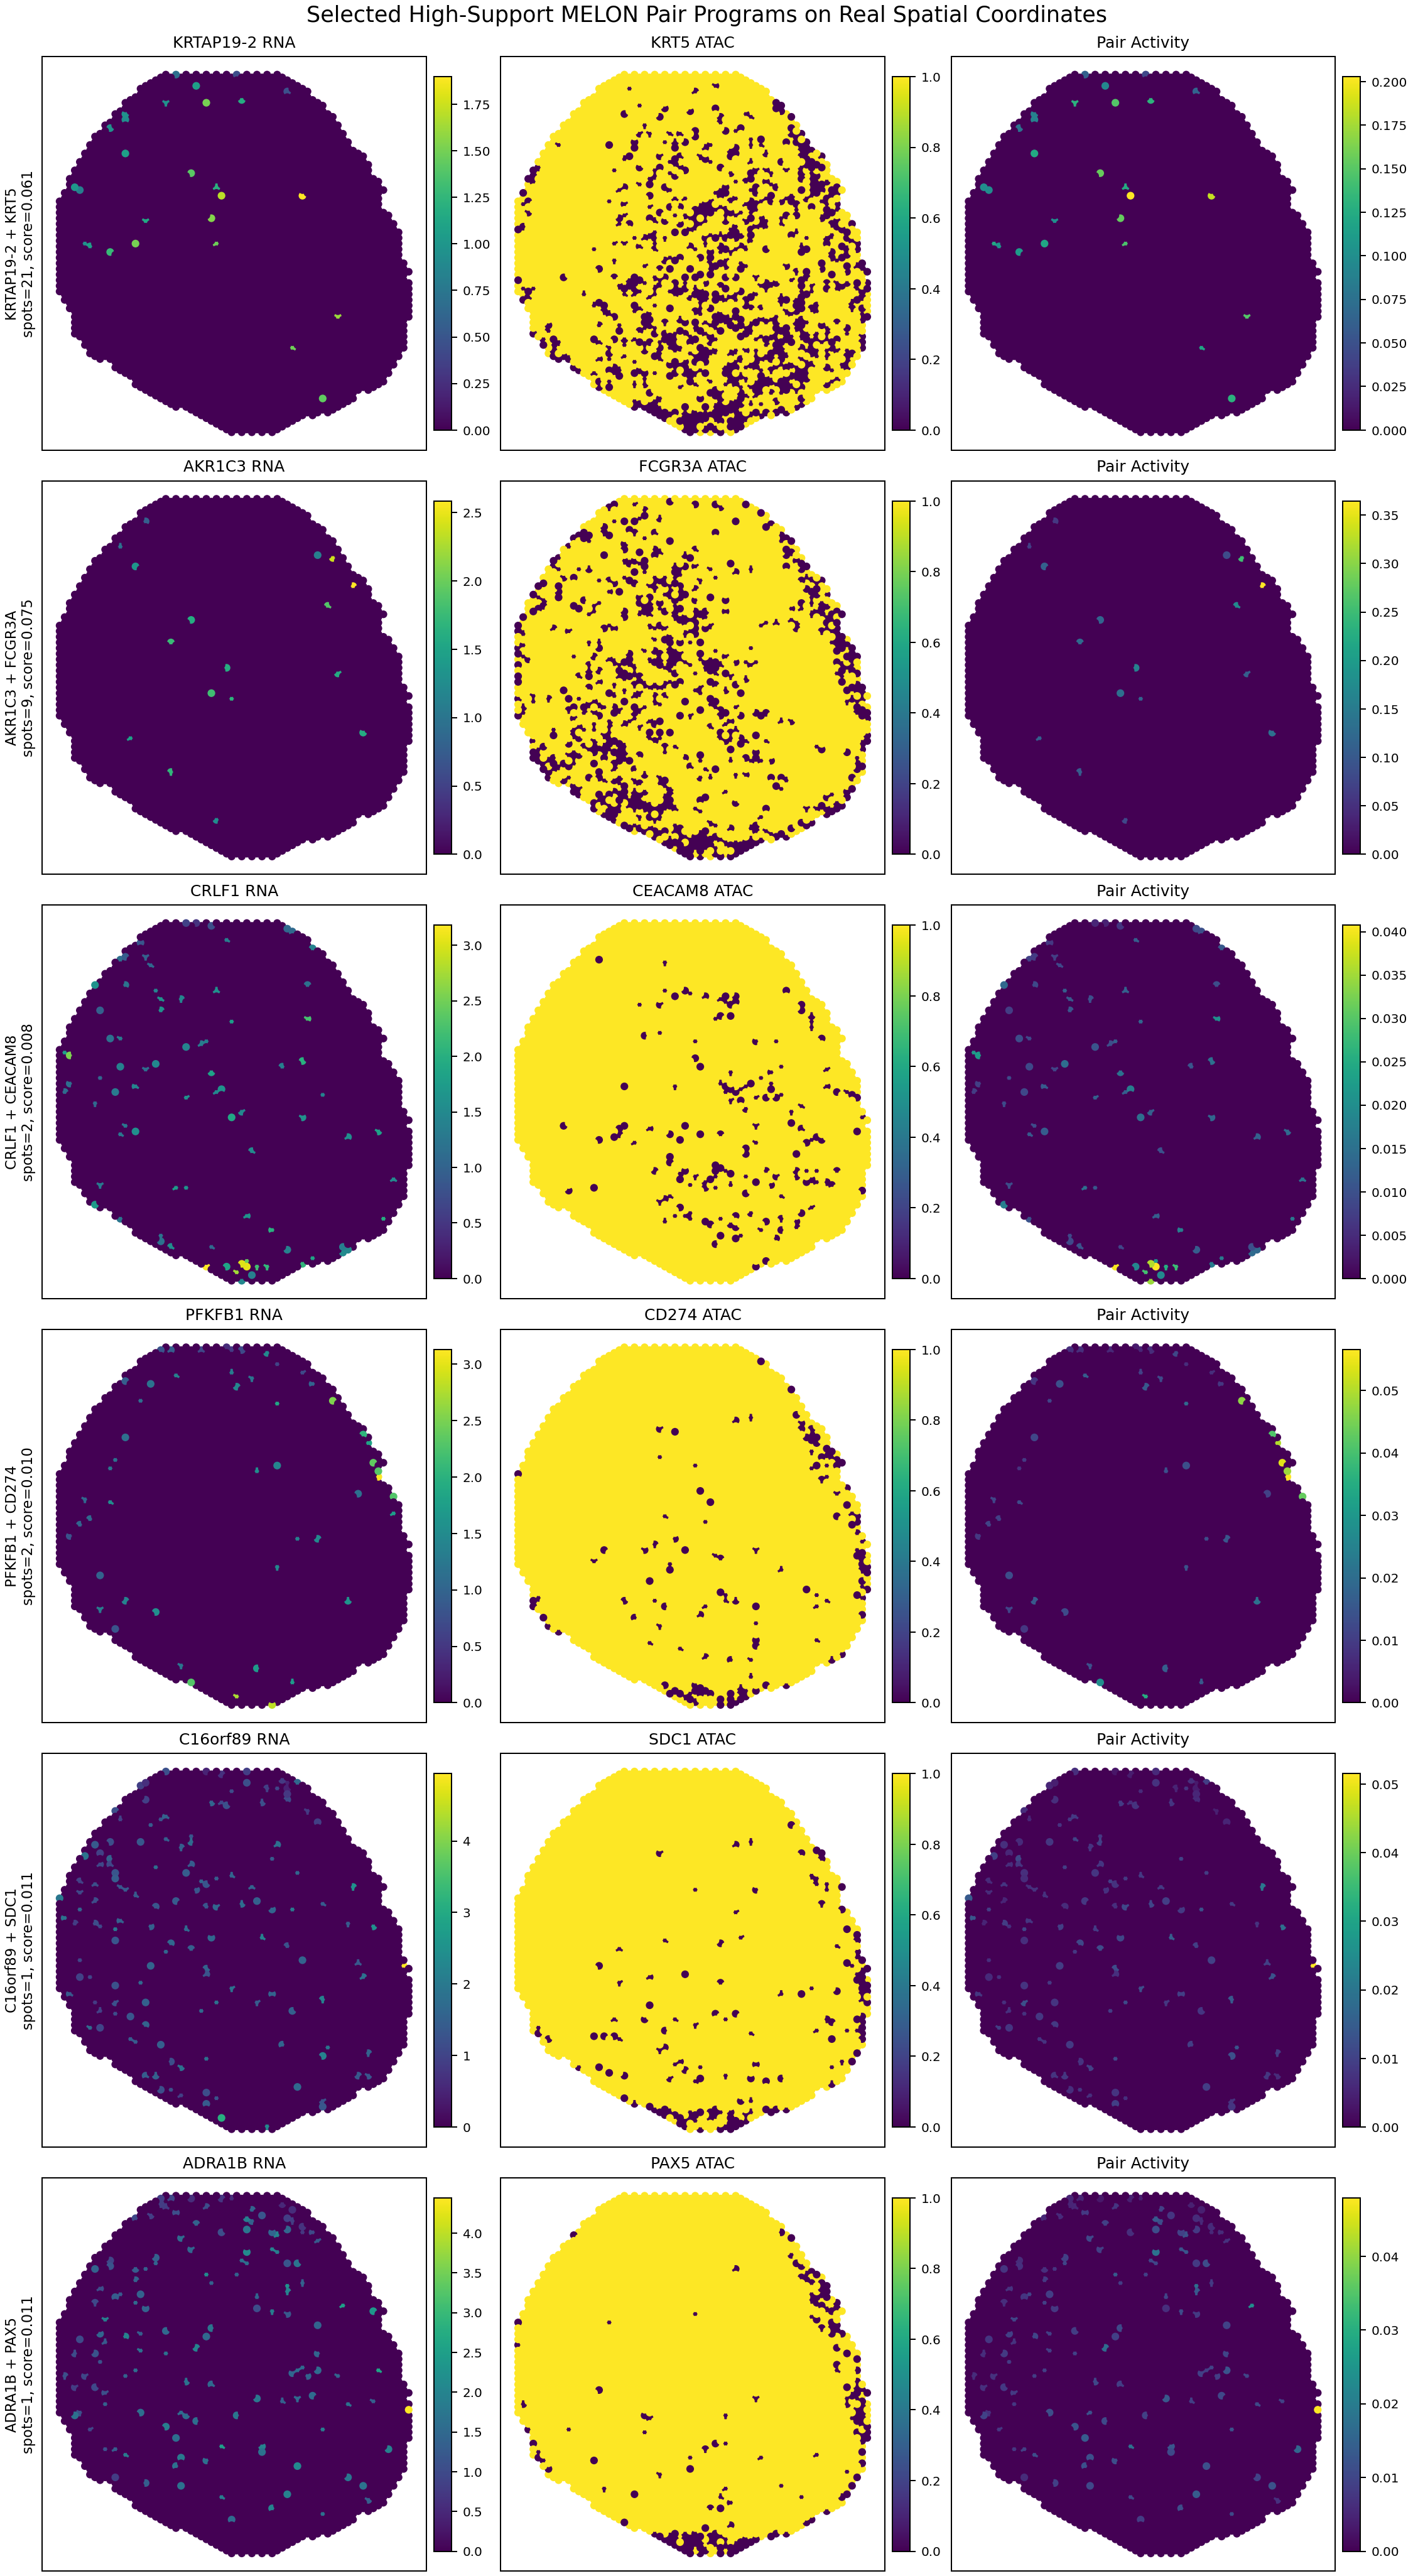
\includegraphics[width=0.75\textwidth]{figures/human_lymph_decoder_pair_maps.png}
\caption{Human lymph node. Spatial maps for six high-support gene--protein pairs from the decoder. Each row is one pair; columns show (left) RNA expression of the gene, (centre) protein (ADT) abundance of the marker, and (right) the decoder's joint pair activity. Selected pairs include canonical immune markers \emph{FCGR3A} (CD16), \emph{CD274} (PD-L1), \emph{SDC1} (CD138, plasma cell), and \emph{PAX5} (B-cell lineage).}
\label{fig:hln-decoder-pairs}
\end{figure}

\begin{figure}[!ht]
\centering
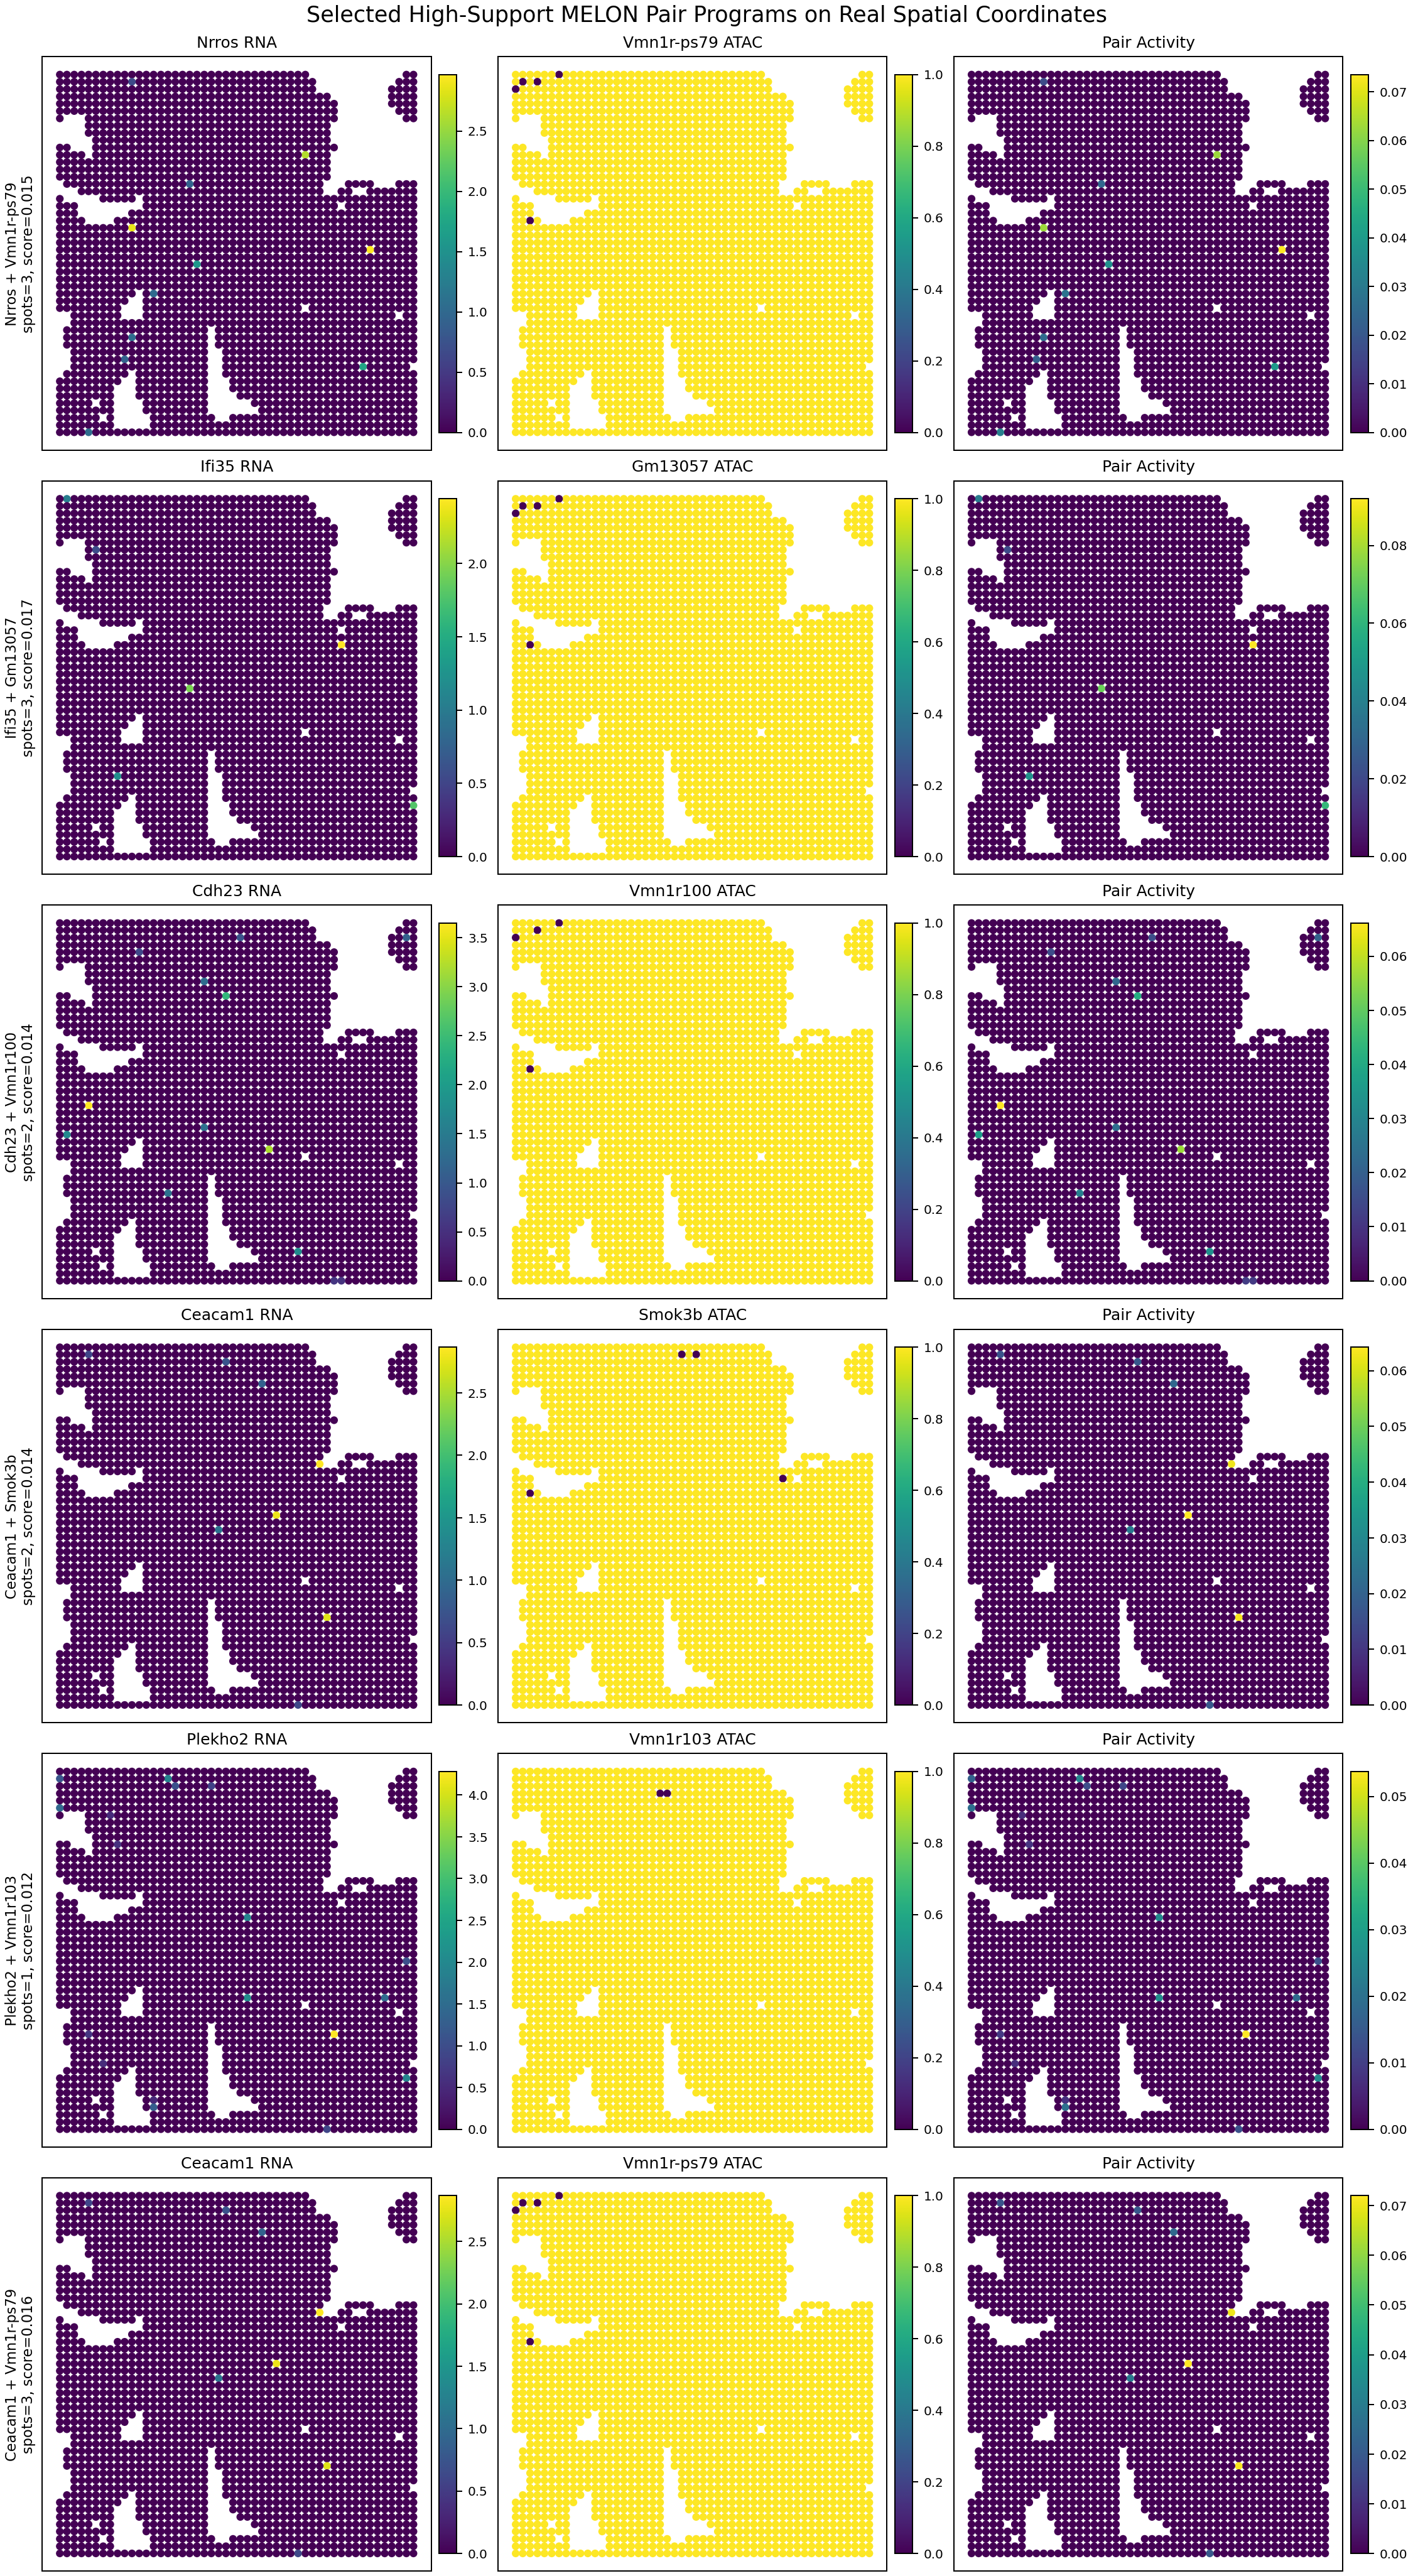
\includegraphics[width=0.75\textwidth]{figures/mouse_embryo_decoder_pair_maps.png}
\caption{Mouse E13 embryo. Spatial maps for six high-support gene--peak pairs from the decoder. Each row is one pair; columns show (left) RNA expression of the gene, (centre) ATAC accessibility of the peak, and (right) the decoder's joint pair activity across all spots.}
\label{fig:embryo-decoder-pairs}
\end{figure}

\subsection{Exploratory Analysis on Datasets Without Ground Truth}\label{app:exploratory}
The three benchmarked datasets in the main text all have expert anatomical annotations, which is the exception rather than the rule for newly profiled spatial multi-omics samples. To illustrate how MELON is used in the more typical \emph{discovery} setting, we apply it without any supervision to two additional samples for which no per-spot ground-truth labels are available: a human hippocampus section profiled with paired RNA and ATAC (2{,}500 spots, 7{,}666 genes) and a clear-cell renal cell carcinoma tumour section (sample Y7\_T) profiled with paired RNA and DNA methylation (2{,}926 spots, 36{,}404 genes). The methylation modality is, to our knowledge, not directly supported by any published spatial multi-omics integration baseline, so MELON is run with the same RNA pipeline and a feature-block configuration analogous to the ATAC head; methylation is treated as a continuous secondary modality. Both runs use the default MELON hyperparameters and Leiden clustering on the fused embedding (resolution chosen to give $k{=}7$ for the hippocampus and $k{=}16$ for the tumour, matching the natural compartment count visible in the H\&E).

\paragraph{Human hippocampus.}
Figure~\ref{fig:exploratory-hippocampus} compares MELON against the seven baselines on this RNA--ATAC sample. MELON, MISO, and SpatialGlue produce contiguous laminar domains that follow the anatomical curvature of the hippocampal formation, while MOFA+, MEFISTO, and TotalVI yield noisier partitions with substantial within-region speckling. The MELON segmentation cleanly separates a putative white-matter band from the granule-cell layer and CA pyramidal cells, suggesting that the same architecture transfers to a brain region with very different tissue geometry from the E15.5 cortical sections used for benchmarking. We do not report ARI here because no per-spot annotation exists for this sample; the figure should be read as a qualitative cross-method comparison.

\paragraph{ccRCC tumour (Y7\_T).}
Figure~\ref{fig:exploratory-ccrcc} shows the same comparison on the renal tumour section. Despite methylation being a markedly different secondary modality from chromatin accessibility, MELON produces large, contiguous tumour and stromal domains rather than scattered spot-level noise. Several baselines either collapse to one or two dominant clusters (TotalVI, MOFA+) or produce highly fragmented partitions that do not respect the visible tumour boundary (MultiGate, MEFISTO). The MELON partition exposes a candidate tumour core surrounded by a thin transitional band and several distinct stromal compartments, motivating downstream analysis of the corresponding gene and methylation programs. As with the hippocampus sample, no expert per-spot annotation is available, so this figure is a discovery-mode result rather than a benchmark.

\begin{figure}[!ht]
\centering
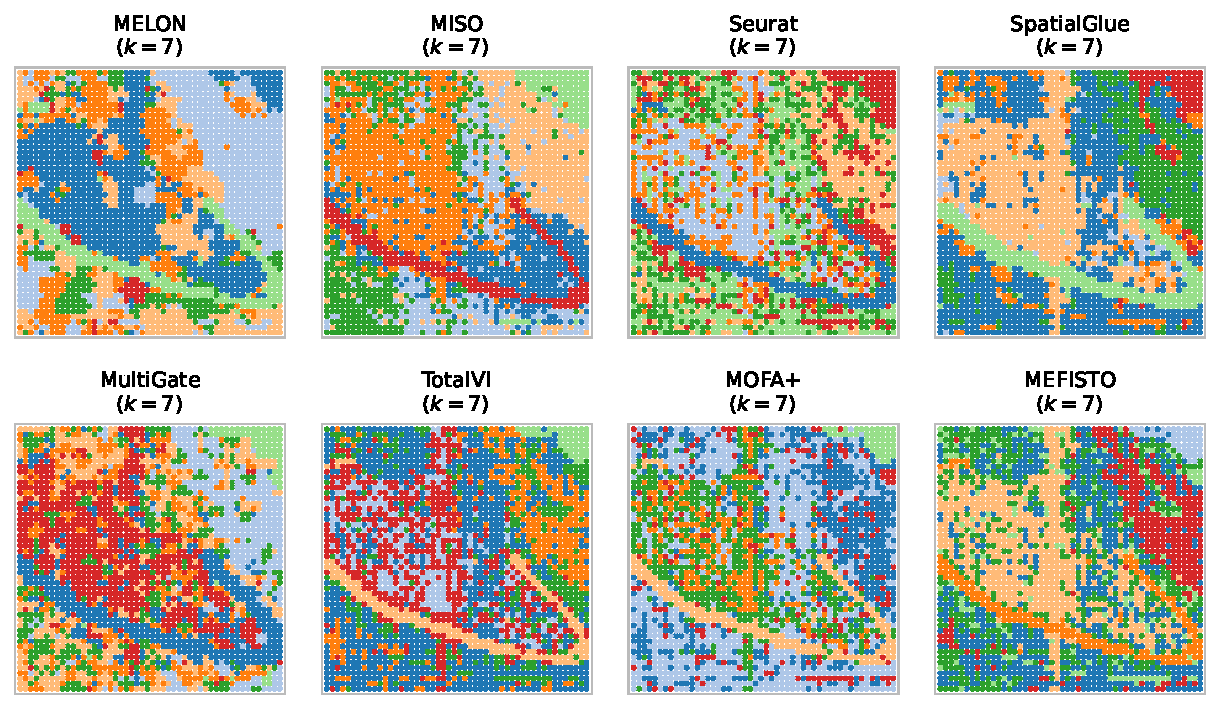
\includegraphics[width=0.95\textwidth]{figures/human_hippocampus_exploratory_panel.pdf}
\caption{Human hippocampus (RNA + ATAC, 2{,}500 spots). Spatial domain assignments from MELON and seven multimodal baselines, each at its natural Leiden resolution ($k$ shown above each panel). No per-spot annotation exists for this sample; panel colours are per-method cluster ids and are not aligned across panels.}
\label{fig:exploratory-hippocampus}
\end{figure}

\begin{figure}[!ht]
\centering
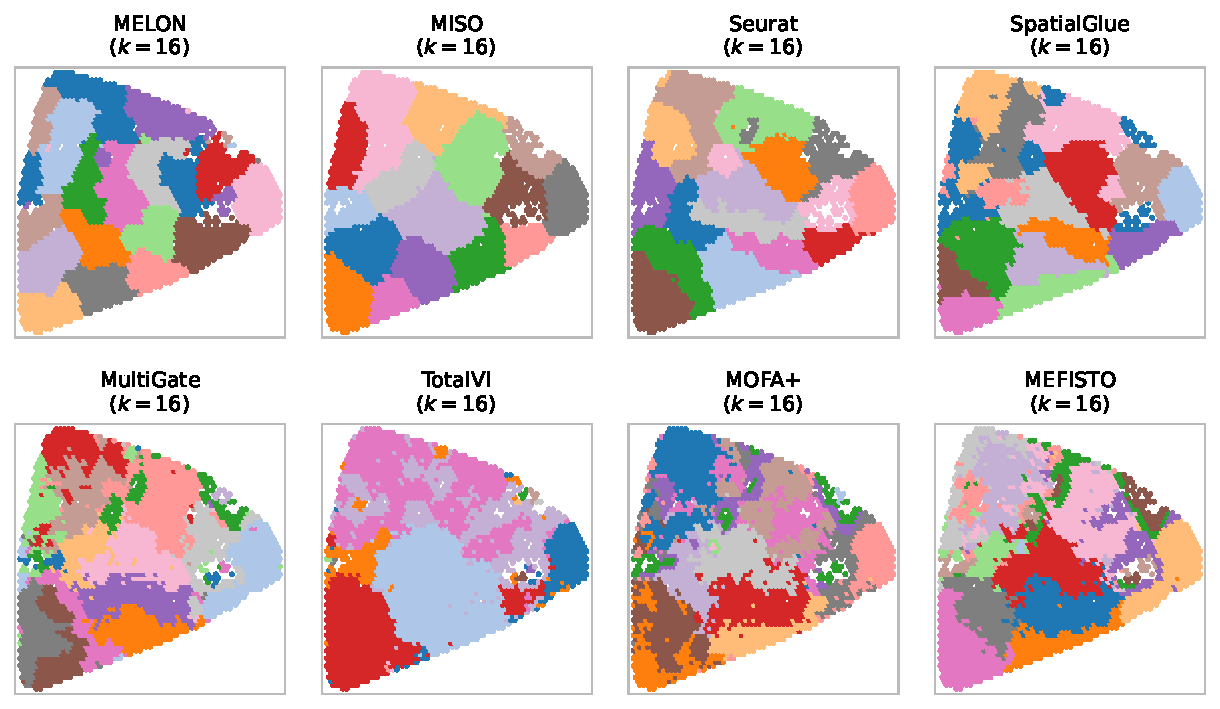
\includegraphics[width=0.95\textwidth]{figures/ccRCC_Y7_T_exploratory_panel.pdf}
\caption{Clear-cell renal cell carcinoma sample Y7\_T (RNA + DNA methylation, 2{,}926 spots). Spatial domain assignments from MELON and seven multimodal baselines at $k{=}16$. Methylation is not a modality directly supported by the baselines; they were run on RNA + a continuous secondary input as a rough analogue. No per-spot annotation exists for this sample; panel colours are per-method cluster ids and are not aligned across panels.}
\label{fig:exploratory-ccrcc}
\end{figure}

% Main-text synergy simulation (tables and figure) is in Section~\ref{sec:simulation}.
% Data generation, simulator validation, and the full seven-variant ablation table
% are in Appendix~\ref{app:sim-design} and Appendix~\ref{app:ablation}.

\section{Simulation Study Details}\label{app:sim-design}

\subsection{Feature Block Architecture}\label{app:feature-blocks}

\begin{table}[!ht]
\centering
\caption{Feature block architecture for each modality. All dimensions sum to 600.}
\label{tab:feature-blocks}
\small
\begin{tabular}{llccl}
\toprule
Modality & Block & Dim & $\sigma$ & Encodes \\
\midrule
\multirow{5}{*}{M1}
 & Shared main     & 150 & 0.5 & $A^{(1)}$ (region-derived) \\
 & Unique task      & 150 & 0.5 & $U$ (M1-specific) \\
 & Nuisance         & 100 & 0.7 & $A^{(3,\text{M1})}$ (confounder) \\
 & Mixed            & 100 & 0.7 & $R + U +$ pair code ($s{=}3.5$) \\
 & Noise            & 100 & 1.0 & $\mathcal{N}(0,1)$ i.i.d. \\
\midrule
\multirow{5}{*}{M2}
 & Shared main     & 150 & 0.5 & $A^{(1)}$ (region-derived) \\
 & Nuisance         & 150 & 0.7 & $A^{(2,\text{M2})}$ (confounder) \\
 & Synergy attr     & 100 & 0.5 & $C$ (M2-specific) \\
 & Mixed            & 100 & 0.7 & $R + C +$ pair code ($s{=}3.5$) \\
 & Noise            & 100 & 1.0 & $\mathcal{N}(0,1)$ i.i.d. \\
\bottomrule
\end{tabular}
\end{table}

\paragraph{Feature generation.}
Each signal block is generated as $\boldsymbol{\mu}_k + \boldsymbol{\epsilon}$, where $\boldsymbol{\mu}_k \sim \mathcal{N}(\mathbf{0}, \sigma^2_\text{centroid}\mathbf{I})$ is a latent-class centroid sampled once per class, and $\boldsymbol{\epsilon} \sim \mathcal{N}(\mathbf{0}, \sigma^2\mathbf{I})$ is independent per-spot noise. The mixed block for each modality combines region structure, modality-specific structure, and a cross-modal pair code:
\begin{align}
    \mathbf{x}^{(1,\text{mixed})}_i &= 0.5\,\boldsymbol{\mu}^{R}_{R_i} + 0.5\,\boldsymbol{\mu}^{U}_{U_i} + s \cdot \boldsymbol{\mu}^{\text{pair}}_{U_i} + \boldsymbol{\epsilon}_i, \label{eq:m1-mixed}\\
    \mathbf{x}^{(2,\text{mixed})}_i &= 0.5\,\boldsymbol{\mu}^{R'}_{R_i} + 0.5\,\boldsymbol{\mu}^{C}_{C_i} + s \cdot \boldsymbol{\mu}^{\text{pair}}_{\pi^{-1}(C_i)} + \boldsymbol{\epsilon}'_i, \label{eq:m2-mixed}
\end{align}
where $s = 3.5$ is the pair-code scale, $\boldsymbol{\mu}^{\text{pair}}_k \sim \mathcal{N}(\mathbf{0}, \mathbf{I})$ is sampled once per attribute code $k$, and $\boldsymbol{\epsilon}_i, \boldsymbol{\epsilon}'_i \sim \mathcal{N}(\mathbf{0}, 0.7^2 \mathbf{I})$. When $C_i = \pi(U_i)$, both modalities share the \emph{same} pair-code vector $\boldsymbol{\mu}^{\text{pair}}_{U_i}$, creating a cross-modal correlation that enables $Y$ recovery from the concatenation but not from either modality alone.

\paragraph{Latent variable sampling.}
Region labels $R_i$ are assigned by Voronoi tessellation of $K_R{=}5$ seed points sampled uniformly on the grid, followed by $T{=}3$ rounds of spatial majority smoothing (8-connected neighbourhood) and stochastic boundary flipping with probability $p_\text{flip}{=}0.05$. The modality-specific attributes $U_i$ and $C_i$ are sampled per region from a region-biased categorical distribution. Within region $r$, the sampling probability over $K{=}10$ attribute codes is
\begin{equation}\label{eq:region-bias}
    \mathbf{p}_r \;=\; (1 - \beta)\,\mathbf{u} \;+\; \beta\,\mathbf{w}_r,
    \qquad
    \mathbf{w}_r \;\sim\; \mathrm{Dir}(\mathbf{1}_K),
    \qquad
    \mathbf{u} \;=\; \tfrac{1}{K}\mathbf{1}_K,
\end{equation}
where $\beta = 0.12$ is the region-bias weight, $\mathbf{w}_r$ is a region-specific Dirichlet draw, and $\mathbf{u}$ is the uniform prior over the $K$ attribute codes. This produces fine-grained within-region heterogeneity that is only weakly correlated with spatial location, so that neither modality alone nor spatial coordinates are sufficient to recover the synergy label $Y$ defined in Eq.~\eqref{eq:y-def}.

\subsection{Simulation Hyperparameters}

\begin{table}[!ht]
\centering
\caption{Complete simulation hyperparameters.}
\label{tab:sim-hyperparams}
\small
\begin{tabular}{llr}
\toprule
Category & Parameter & Value \\
\midrule
Grid        & Size & $44 \times 44$ ($N{=}1{,}936$) \\
\midrule
Latent      & Regions $K_R$ & 5 \\
            & Shared attr.\ levels $K_{A_1}$ & 5 \\
            & M1-specific levels $K_U$ & 10 \\
            & M2-specific levels $K_C$ & 10 \\
            & Nuisance levels & 8 \\
            & Region bias $\beta$ & 0.12 \\
\midrule
Synergy     & Match prob $p_\text{match}$ & 0.90 \\
            & Non-match prob $p_\text{non}$ & 0.01 \\
            & Pair-code scale $s$ & 3.5 \\
\midrule
Noise       & $\sigma_\text{shared}$, $\sigma_\text{task}$ & 0.5 \\
            & $\sigma_\text{nuisance}$, $\sigma_\text{mixed}$ & 0.7 \\
            & $\sigma_\text{noise}$ & 1.0 \\
            & $\sigma_\text{centroid}$ (main / nuisance) & 2.0 / 1.5 \\
\midrule
Spatial     & Smoothing iterations $T$ & 3 \\
            & Shared flip prob & 0.05 \\
            & Attribute flip prob & 0.05 \\
            & Nuisance flip prob & 0.08 \\
\midrule
            & Random seed & 123 \\
\bottomrule
\end{tabular}
\end{table}

\subsection{Spatial Structure of Simulated Data}\label{app:spatial}

Figure~\ref{fig:spatial-heatmaps} visualizes the spatial distribution of all latent variables on the $44 \times 44$ grid.
Region labels $R$ form coarse spatial domains from Voronoi tessellation.
The modality-specific attributes $U$ and $C$ exhibit finer within-region heterogeneity due to weak region bias ($\beta = 0.12$).
The synergy label $Y$ shows no obvious spatial pattern, confirming that it cannot be trivially predicted from location.

\begin{figure}[!ht]
\centering
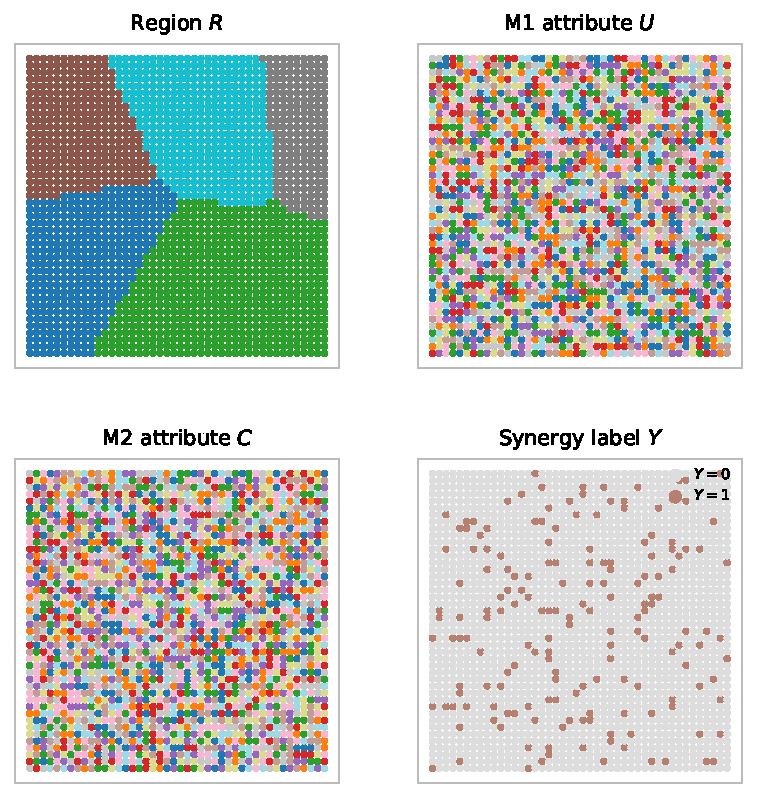
\includegraphics[width=0.55\textwidth]{figures/sim_spatial_heatmaps.pdf}
\caption{Spatial distribution of latent variables on the $44\times44$ simulation grid. Region label $R$ forms coarse Voronoi domains; the modality-specific attributes $U$ and $C$ are fine-grained with weak region bias; the synergy label $Y$ shows no apparent spatial structure (orange = $Y{=}1$).}
\label{fig:spatial-heatmaps}
\end{figure}

\begin{figure}[!ht]
\centering
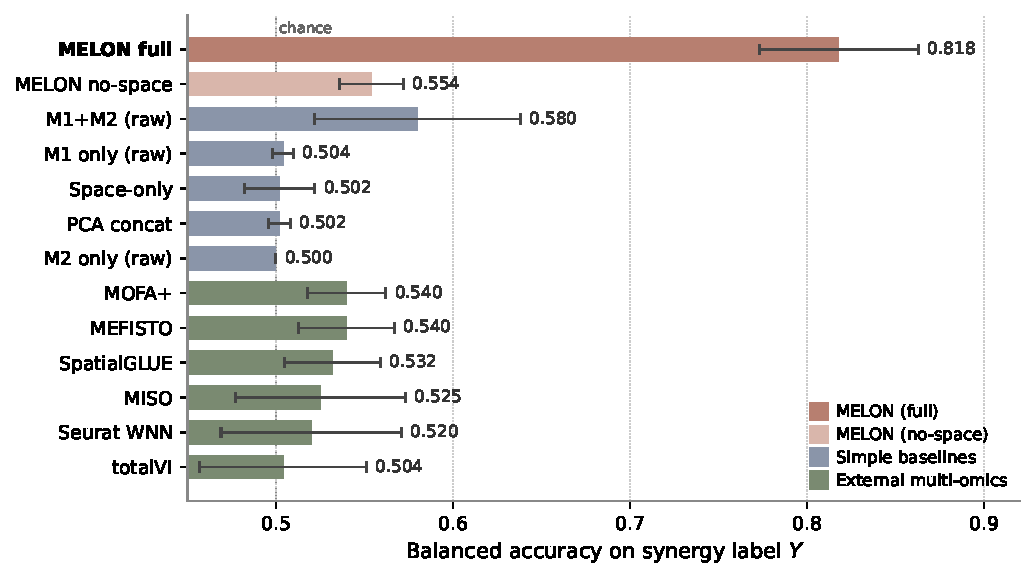
\includegraphics[width=0.85\textwidth]{figures/sim_method_comparison.pdf}
\caption{Method comparison on synergy label $Y$ (balanced accuracy, best probe per method, 5-fold CV). MELON (full) is the only method that meaningfully exceeds chance, while every simple baseline and external multi-omics method stays at or below $0.58$. The \emph{no-space} MELON ablation (lighter accent) collapses to baseline level, showing that the gain depends on spatial conditioning rather than fusion alone. Visualizes the numbers in Table~\ref{tab:sim-phase2}.}
\label{fig:sim-results}
\end{figure}

\subsection{Embedding Visualization}\label{app:embedding}

\begin{figure}[!ht]
\centering
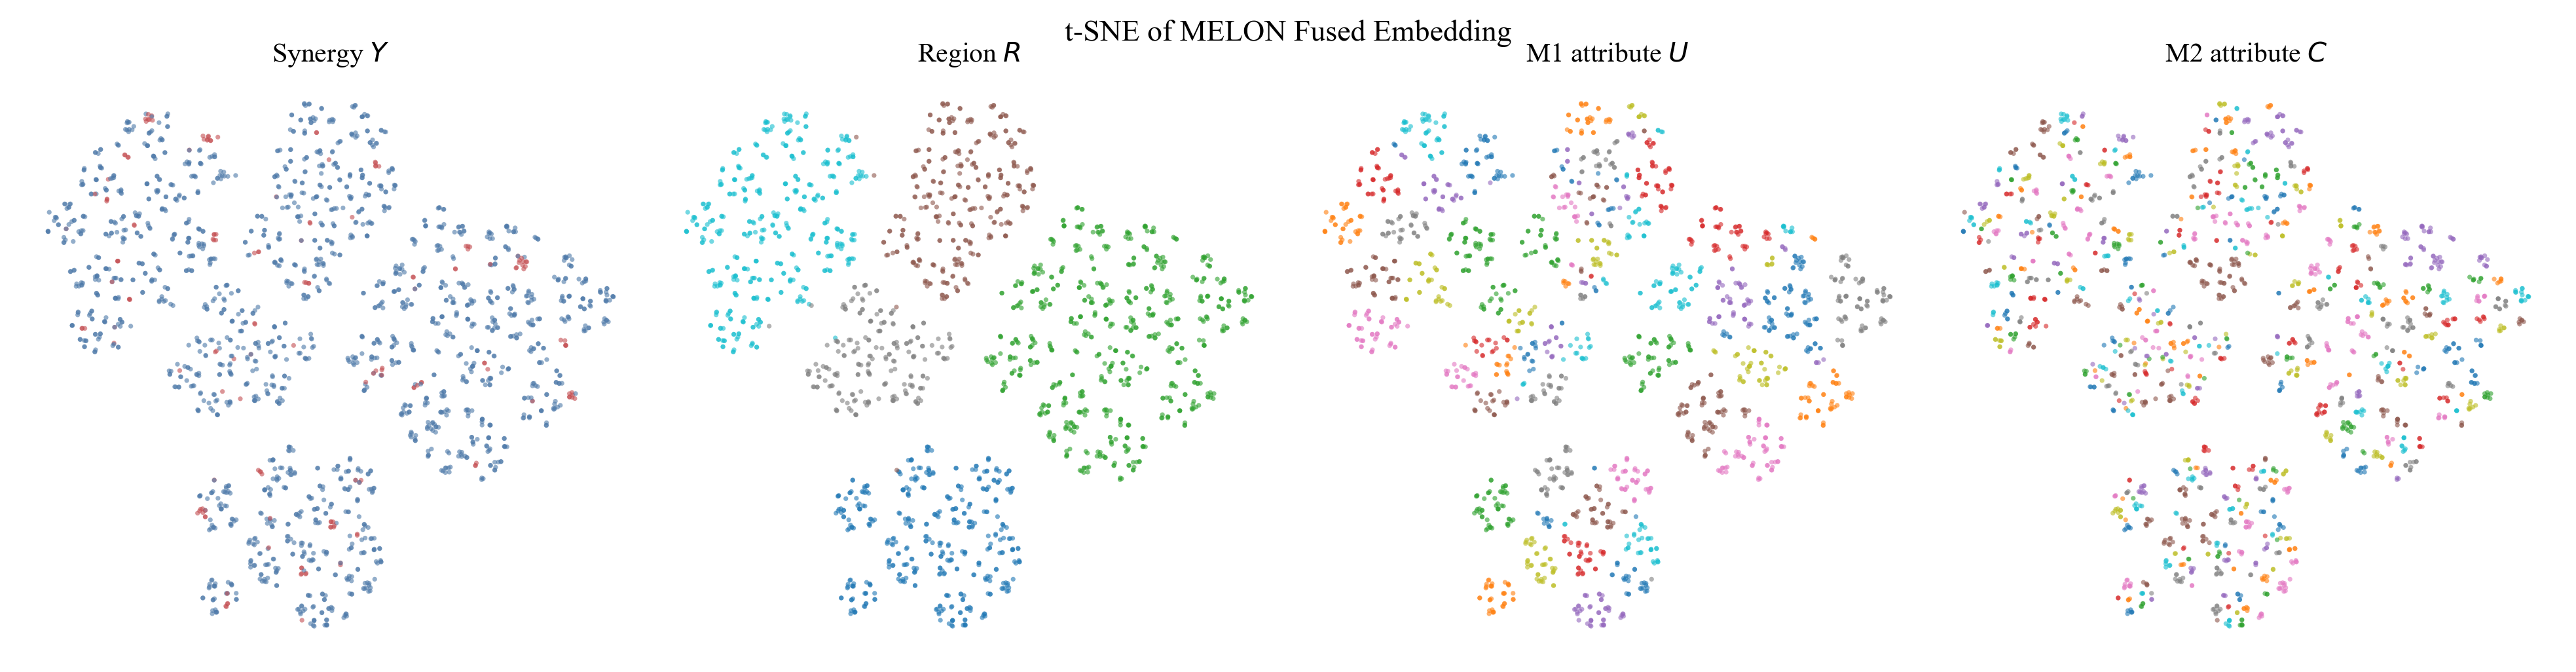
\includegraphics[width=\textwidth]{figures/fig_sim_tsne_embedding.png}
\caption{t-SNE of \melon{} fused embedding colored by synergy label $Y$, region $R$, M1 attribute $U$, and M2 attribute $C$.}
\label{fig:tsne}
\end{figure}

\subsection{Cross-Target Probe Comparison}\label{app:cross-target}

Figure~\ref{fig:probe-heatmap} compares balanced accuracy across all methods and prediction targets.
External multi-omics methods achieve near-perfect recovery of shared structure ($R$) and modality-specific attributes ($U$, $C$) but uniformly fail on the synergy label $Y$.
\melon{} is the only method that achieves above-chance performance on $Y$.

\begin{figure}[!ht]
\centering
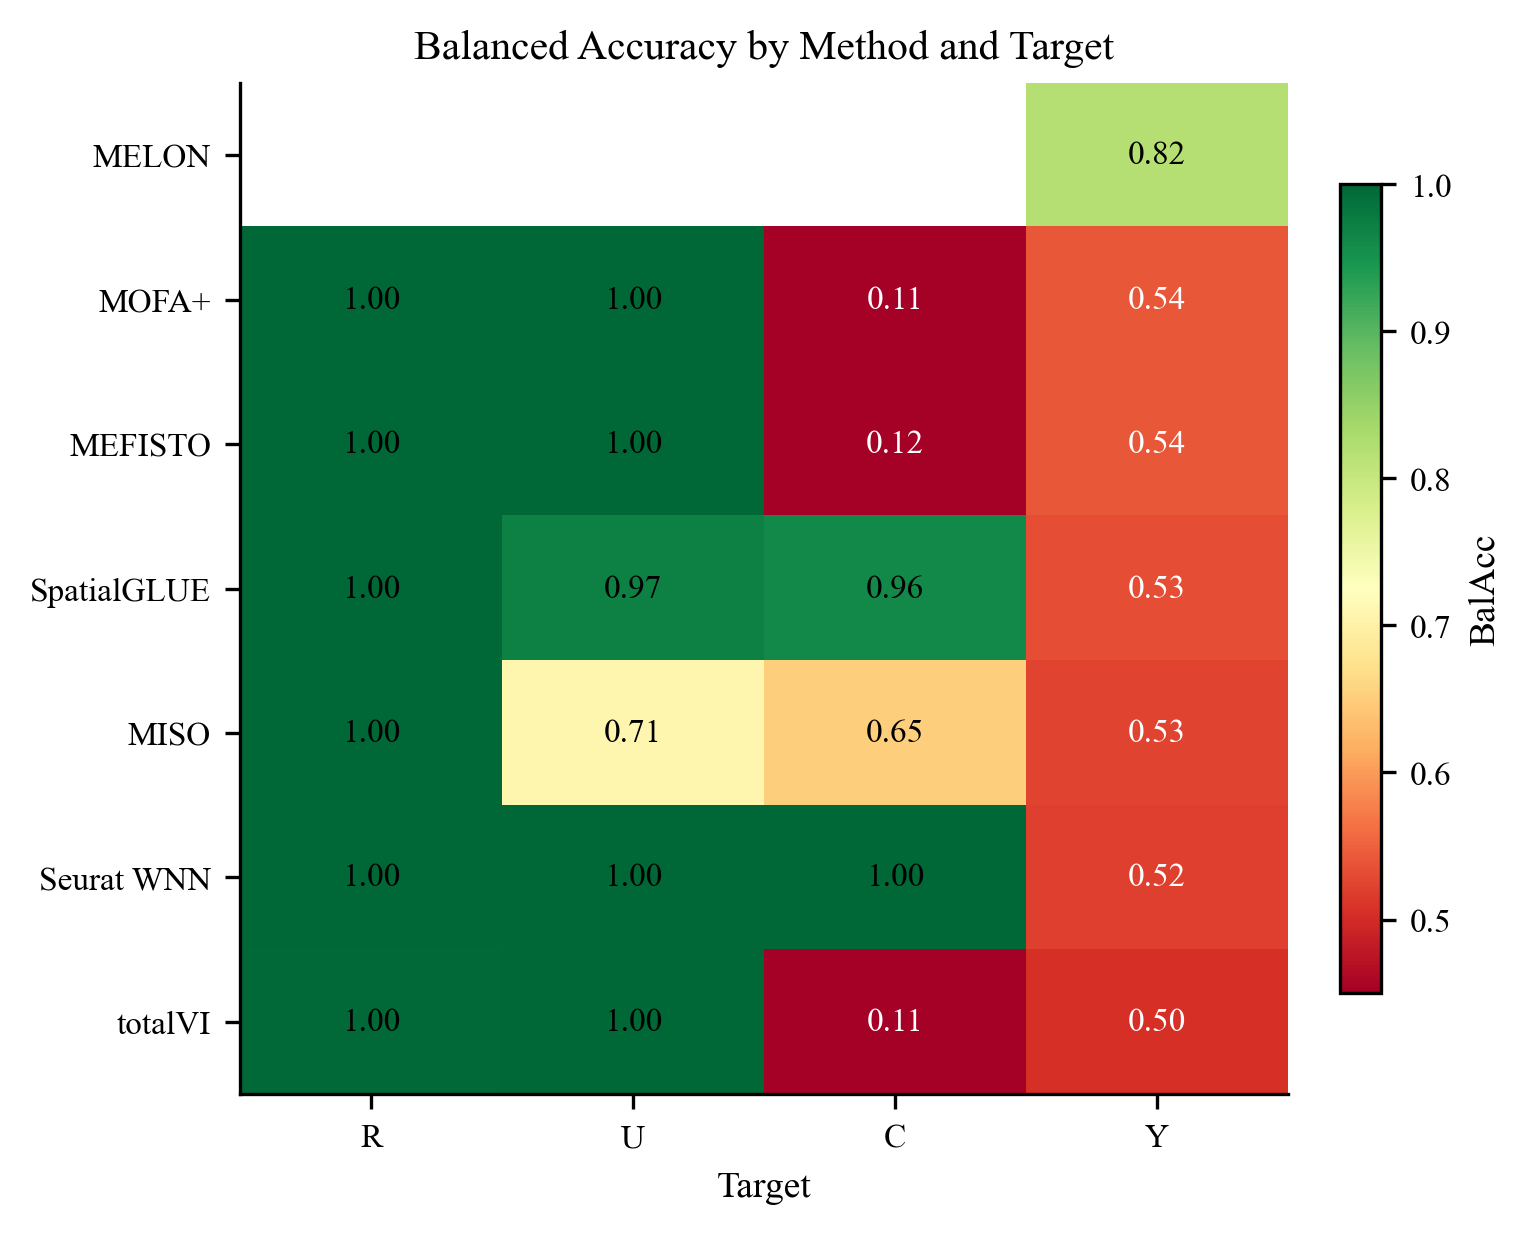
\includegraphics[width=0.55\textwidth]{figures/fig_sim_probe_heatmap.png}
\caption{Balanced accuracy by method and target. External methods recover $R$, $U$, $C$ but not $Y$; \melon{} is the only method with above-chance $Y$ recovery.}
\label{fig:probe-heatmap}
\end{figure}

\subsection{Simulation Validation}\label{app:validation}

We verify four properties of the simulator using 5-fold cross-validated classifiers (logistic regression, random forest, MLP).

\paragraph{Block recoverability.}
Each feature block should encode its intended latent variable. Informative blocks achieve balanced accuracy $\geq 0.85$ on their designated targets, while noise blocks remain at chance ($\leq 0.52$; Table~\ref{tab:sim-phase1-block}).

\paragraph{Synergy validity.}
$Y$ should not be recoverable from a single modality. M1-only and M2-only classifiers achieve balanced accuracy $\leq 0.52$, while the concatenation of both modalities reaches $0.632 \pm 0.027$ (Table~\ref{tab:sim-phase1-synergy}).

\paragraph{Spatial leakage.}
$Y$ should not be predictable from coordinates alone. Coordinate-only classifiers achieve $0.521 \pm 0.011$, confirming negligible spatial leakage (Table~\ref{tab:sim-phase1-spatial}).

\paragraph{Acceptance.}
All criteria are met: informative blocks dominate, noise is at chance, $Y$ requires both modalities, and spatial location alone is uninformative about $Y$.

\begin{table}[!ht]
\centering
\caption{Block recoverability (selected results). Balanced accuracy, 5-fold CV.}
\label{tab:sim-phase1-block}
\small
\begin{tabular}{llcc}
\toprule
Modality & Block $\to$ Target & Best Model & BalAcc \\
\midrule
M1   & Shared $\to$ $R$       & LogReg & $1.000 \pm 0.000$ \\
M1   & Unique $\to$ $U$       & LogReg & $1.000 \pm 0.000$ \\
M1   & Noise $\to$ $Y$        & LogReg & $0.520 \pm 0.021$ \\
M2   & Shared $\to$ $R$       & LogReg & $1.000 \pm 0.000$ \\
M2   & Synergy attr $\to$ $C$ & LogReg & $1.000 \pm 0.000$ \\
M2   & Noise $\to$ $Y$        & RF     & $0.522 \pm 0.011$ \\
\bottomrule
\end{tabular}
\end{table}

\begin{table}[!ht]
\centering
\caption{Synergy validity. Predicting $Y$ from raw features; 5-fold CV, best classifier per row.}
\label{tab:sim-phase1-synergy}
\small
\begin{tabular}{lccc}
\toprule
Input & BalAcc & Macro-F1 & AUROC \\
\midrule
M1 only       & $0.518 \pm 0.008$ & $0.517 \pm 0.008$ & $0.532 \pm 0.008$ \\
M2 only       & $0.504 \pm 0.017$ & $0.504 \pm 0.017$ & $0.520 \pm 0.023$ \\
M1 + M2       & $\mathbf{0.632 \pm 0.027}$ & $\mathbf{0.631 \pm 0.028}$ & $\mathbf{0.672 \pm 0.039}$ \\
\bottomrule
\end{tabular}
\end{table}

\begin{table}[!ht]
\centering
\caption{Spatial leakage test. Predicting $Y$ from spatial features only; 5-fold CV.}
\label{tab:sim-phase1-spatial}
\small
\begin{tabular}{lcc}
\toprule
Input & Best Model & BalAcc \\
\midrule
Coordinates only          & LogReg & $0.521 \pm 0.011$ \\
Neighborhood summary      & LogReg & $0.496 \pm 0.016$ \\
Coords + neighborhood     & RF     & $0.513 \pm 0.021$ \\
\bottomrule
\end{tabular}
\end{table}

\FloatBarrier
\subsection{Full Ablation Results}\label{app:ablation}

\begin{figure}[!ht]
\centering
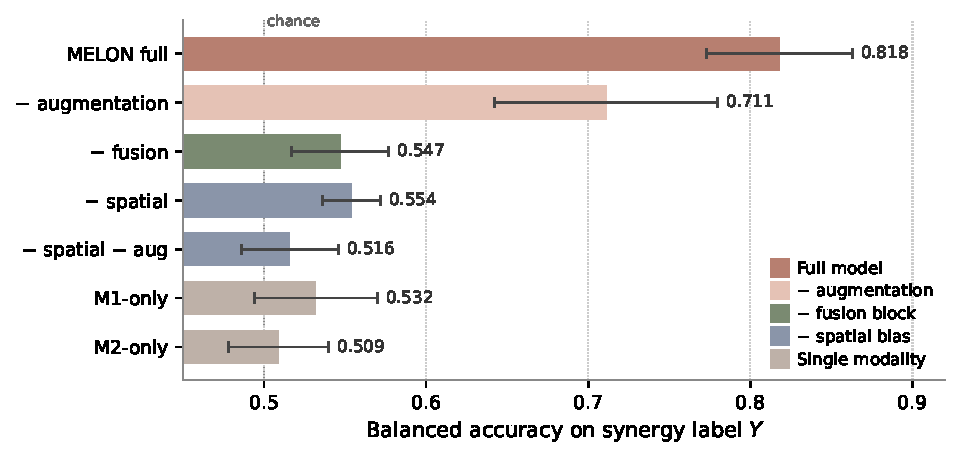
\includegraphics[width=0.75\textwidth]{figures/sim_ablation.pdf}
\caption{Ablation on synergy label $Y$ (balanced accuracy, 5-fold CV). Bars are coloured by ablation axis. Removing the fusion block or the spatial bias each collapses performance to near chance, while augmentation contributes a smaller but consistent gain.}
\label{fig:ablation-full}
\end{figure}

\begin{table}[!ht]
\centering
\caption{Full ablation on $Y$. All variants use the best probe (encoder-stage MLP for spatial variants, linear SVM otherwise). 5-fold CV.}
\label{tab:sim-phase3-ablation-full}
\resizebox{\textwidth}{!}{%
\begin{tabular}{lccccccc}
\toprule
Variant & Input & Fusion & Spatial & Aug & BalAcc & Macro-F1 & AUROC \\
\midrule
\melon{} full              & Multi & \checkmark & \checkmark & 0.3 & $\mathbf{0.818 \pm 0.045}$ & $\mathbf{0.854 \pm 0.034}$ & $\mathbf{0.955 \pm 0.021}$ \\
\melon{} full (no aug)     & Multi & \checkmark & \checkmark & 0.0 & $0.711 \pm 0.069$ & $0.765 \pm 0.068$ & $0.906 \pm 0.047$ \\
\melon{} no-fusion         & Multi & ---        & ---        & 0.3 & $0.547 \pm 0.030$ & $0.504 \pm 0.018$ & $0.573 \pm 0.028$ \\
\melon{} no-space          & Multi & \checkmark & ---        & 0.3 & $0.554 \pm 0.018$ & $0.504 \pm 0.011$ & $0.576 \pm 0.034$ \\
\melon{} no-space (no aug) & Multi & \checkmark & ---        & 0.0 & $0.516 \pm 0.030$ & $0.486 \pm 0.013$ & $0.542 \pm 0.052$ \\
\melon{} M1-only            & M1   & \checkmark & \checkmark & 0.0 & $0.532 \pm 0.038$ & $0.489 \pm 0.024$ & $0.511 \pm 0.053$ \\
\melon{} M2-only            & M2   & \checkmark & \checkmark & 0.0 & $0.509 \pm 0.031$ & $0.476 \pm 0.015$ & $0.524 \pm 0.027$ \\
\bottomrule
\end{tabular}%
}
\end{table}

%%%%%%%%%%%%%%%%%%%%%%%%%%%%%%%%%%%%%%%%%%%%%%%%%%%%%%%%%%%%
\FloatBarrier

\section{Limitations}\label{app:limitations}

MELON has been evaluated on five spatial multi-omics datasets (three benchmarked, two exploratory) with $n=2$ modalities; its behaviour under three or more modalities, substantially larger tissue sections, or 3D spatial coordinates remains untested. The fusion transformer uses a single layer with embedding width 128, which limits the model's capacity to saturate the InfoNCE bound (Appendix~\ref{app:proof}), so the recovered PID components are a lower bound rather than an exact decomposition. The label-preserving augmentation assumption underlying the theoretical guarantee holds only approximately for the augmentations we use, and may degrade for modalities with very different noise characteristics. Finally, the $k$-NN spatial graph is constructed from Euclidean coordinates and does not account for physical barriers such as tissue boundaries or folds, which could introduce spurious spatial edges.

\end{document}

